% APPENDIX
\chapter{$Z\gamma$ Check}
\label{sec:ZgCheck}

The poor agreement in all distributions of $W\gamma$ candidates in Ch.~\ref{sec:BackgroundSubtraction_results} brought up the necessity of cross checks that would help to identify the sources of the disagreements. One of such cross checks is the $Z\gamma$ check which is the $Z\gamma$ cross section measurement performed following the same strategy as used for the $W\gamma$ cross section measurement (Ch.~\ref{sec:AN_WgMeasStrategy}). In addition to the comparison of results of jets$\rightarrow\gamma$ background estimation provided by two different methods, the measured $Z\gamma$ cross section is compared to the CMS published $Z\gamma$ cross section at~8~TeV~\cite{ref_Zg8TeV}. The comparison of the cross section to the independently obtained result provides the check for all $W\gamma$ measurement steps except those that are not relevant for the $Z\gamma$ measurement like $e\rightarrow\gamma$ and real-$\gamma$ background estimation, selection requirements on $M_T^W$ and $M_{e\gamma}$, corrections for ``PixelSeedVeto'' SF. 

The $Z\gamma$ events selection is described in Ch.~\ref{sec:AN_Selection_EventLevel}, and the $P_T^{\gamma}$ distribution of $Z\gamma$ candidates in data and MC is shown in Fig.~\ref{fig:DATAvsMC_Zg}. The selected sample mostly consists of $Z\gamma$ signal and DY+jets background events. DY+jets background is a source of jets$\rightarrow\gamma$ background and is estimated the same way as it is done for our nominal $W\gamma$ measurement.  

The templates are derived from $Z\gamma\rightarrow\mu\mu\gamma$ sample. Therefore, the $Z\gamma$ check in the muon channel is not a valid physics measurement but a closure check because the templates for the jets$\rightarrow\gamma$ background estimation procedure largely overlap with the fitted data. At the same time, the $Z\gamma$ check in the electron channel is a valid physics measurement. Fit results on data and pseudodata (MC mixtures) show good agreement for both channels (Fig.~\ref{fig:DDvsMC_Zg_Data_MUON}-\ref{fig:DDvsMC_Zg_MCclosure_ELECTRON}). %The fit plots themselves are available in App.~\ref{sec:TemplateFitPlotsZGamma}-\ref{sec:TemplateFitPlotsMCclosure_ZGamma}.

Major systematic uncertainties are estimated the same way as it is done for $W\gamma$ measurement and are listed in Tab.~\ref{tab:systInPercent_MUON_ZGamma}-\ref{tab:systInPercent_ELECTRON_ZGamma}. Measured cross section values compared to the MC-based cross section are listed in the Tab.~\ref{tab:cs_mc_vs_meas_ZGamma}. Figure~\ref{fig:CS_Zg} shows an agreement between muon and electron channels, agreement with the MC-based cross section and with the published CMS $Z\gamma$ measurement at $\sqrt{s}=$8~TeV~\cite{ref_Zg8TeV}.

The good agreement between the $Z\gamma$ cross section of our measurement and the published one validates steps of the $W\gamma$ measurement that are the same between $Z\gamma$ and $W\gamma$ measurements. The list of the same steps includes muon, electron, and photon selection, jets$\rightarrow\gamma$ background estimation, detector resolution unfolding, acceptance, efficiency, and SF corrections, PU reweighting.

\begin{figure}[htb]
  \begin{center}
   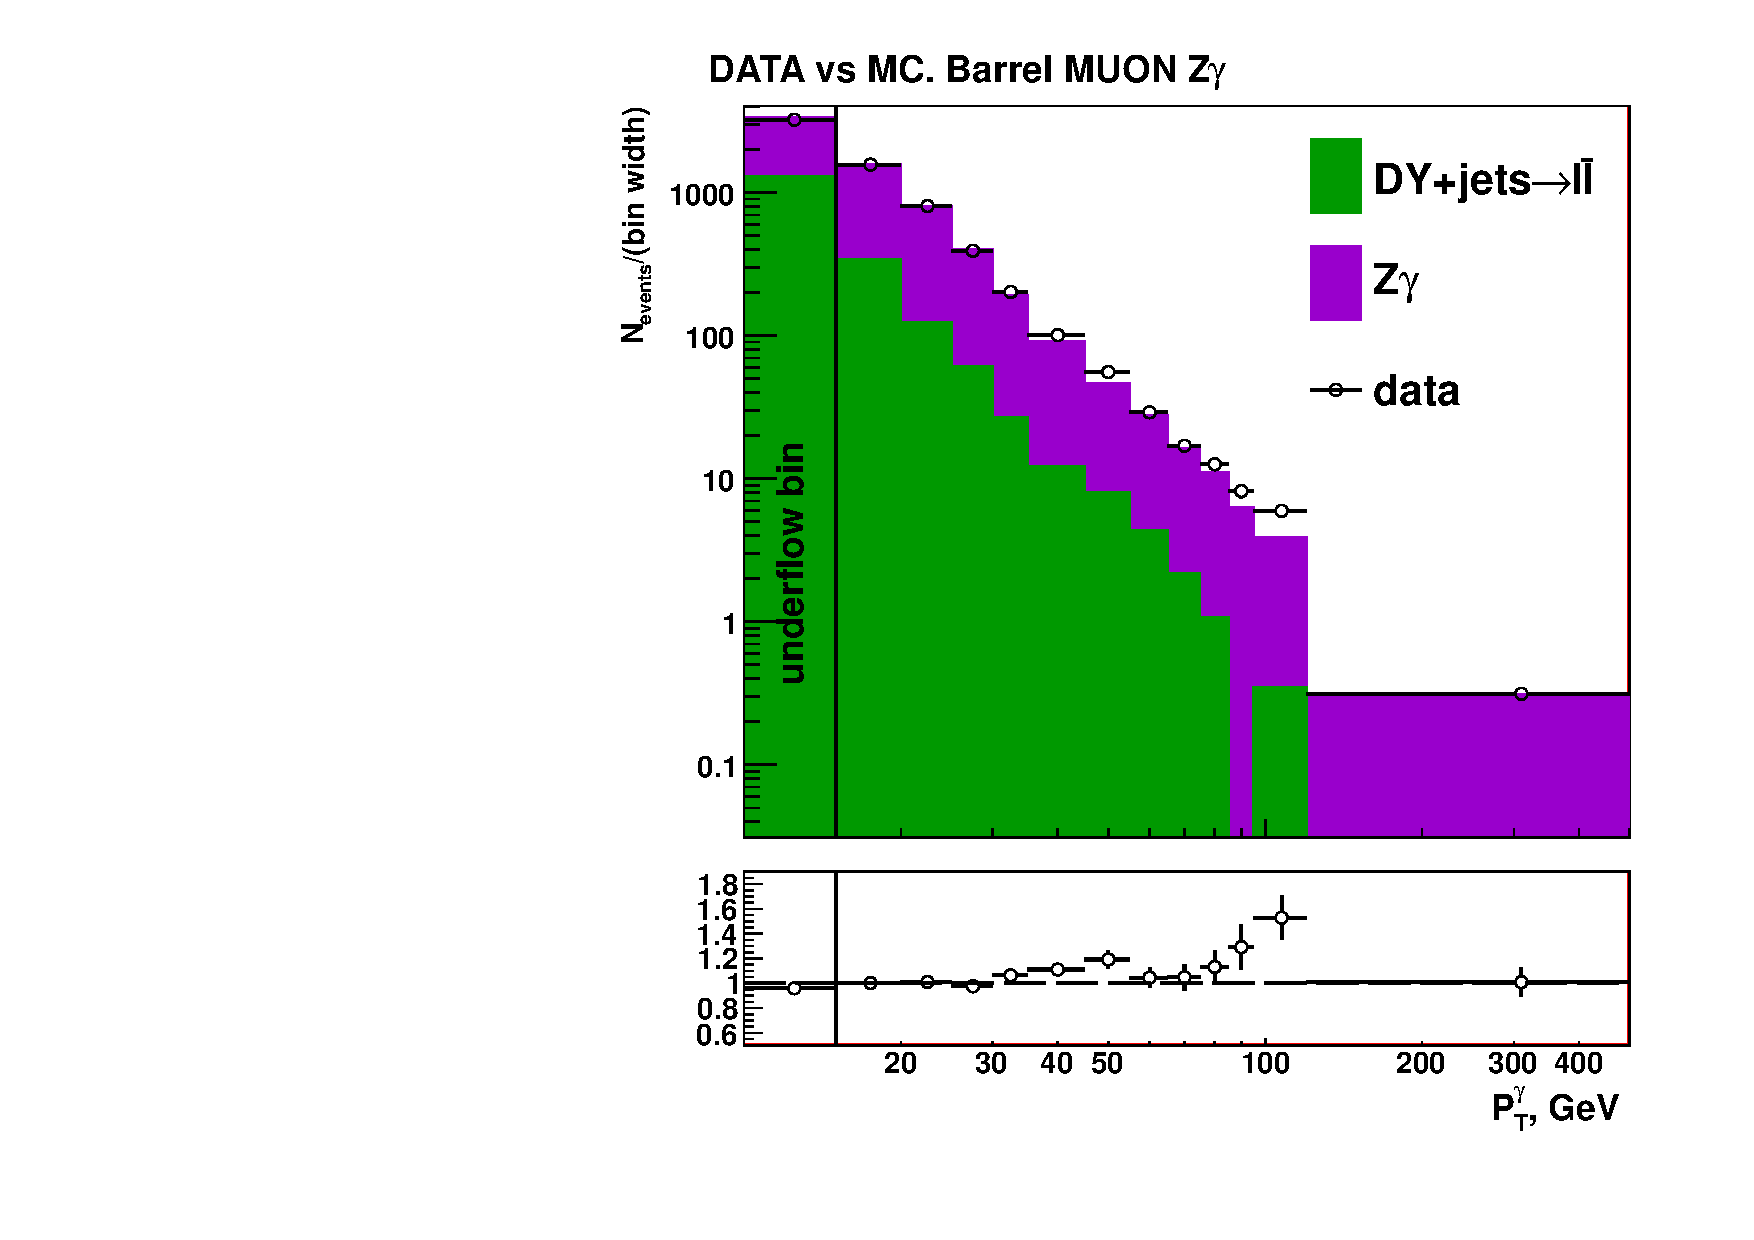
\includegraphics[width=0.45\textwidth]{../figs/figs_v11/MUON_ZGamma/PrepareYields/c_TotalDATAvsMC_Barrel__phoEt.pdf}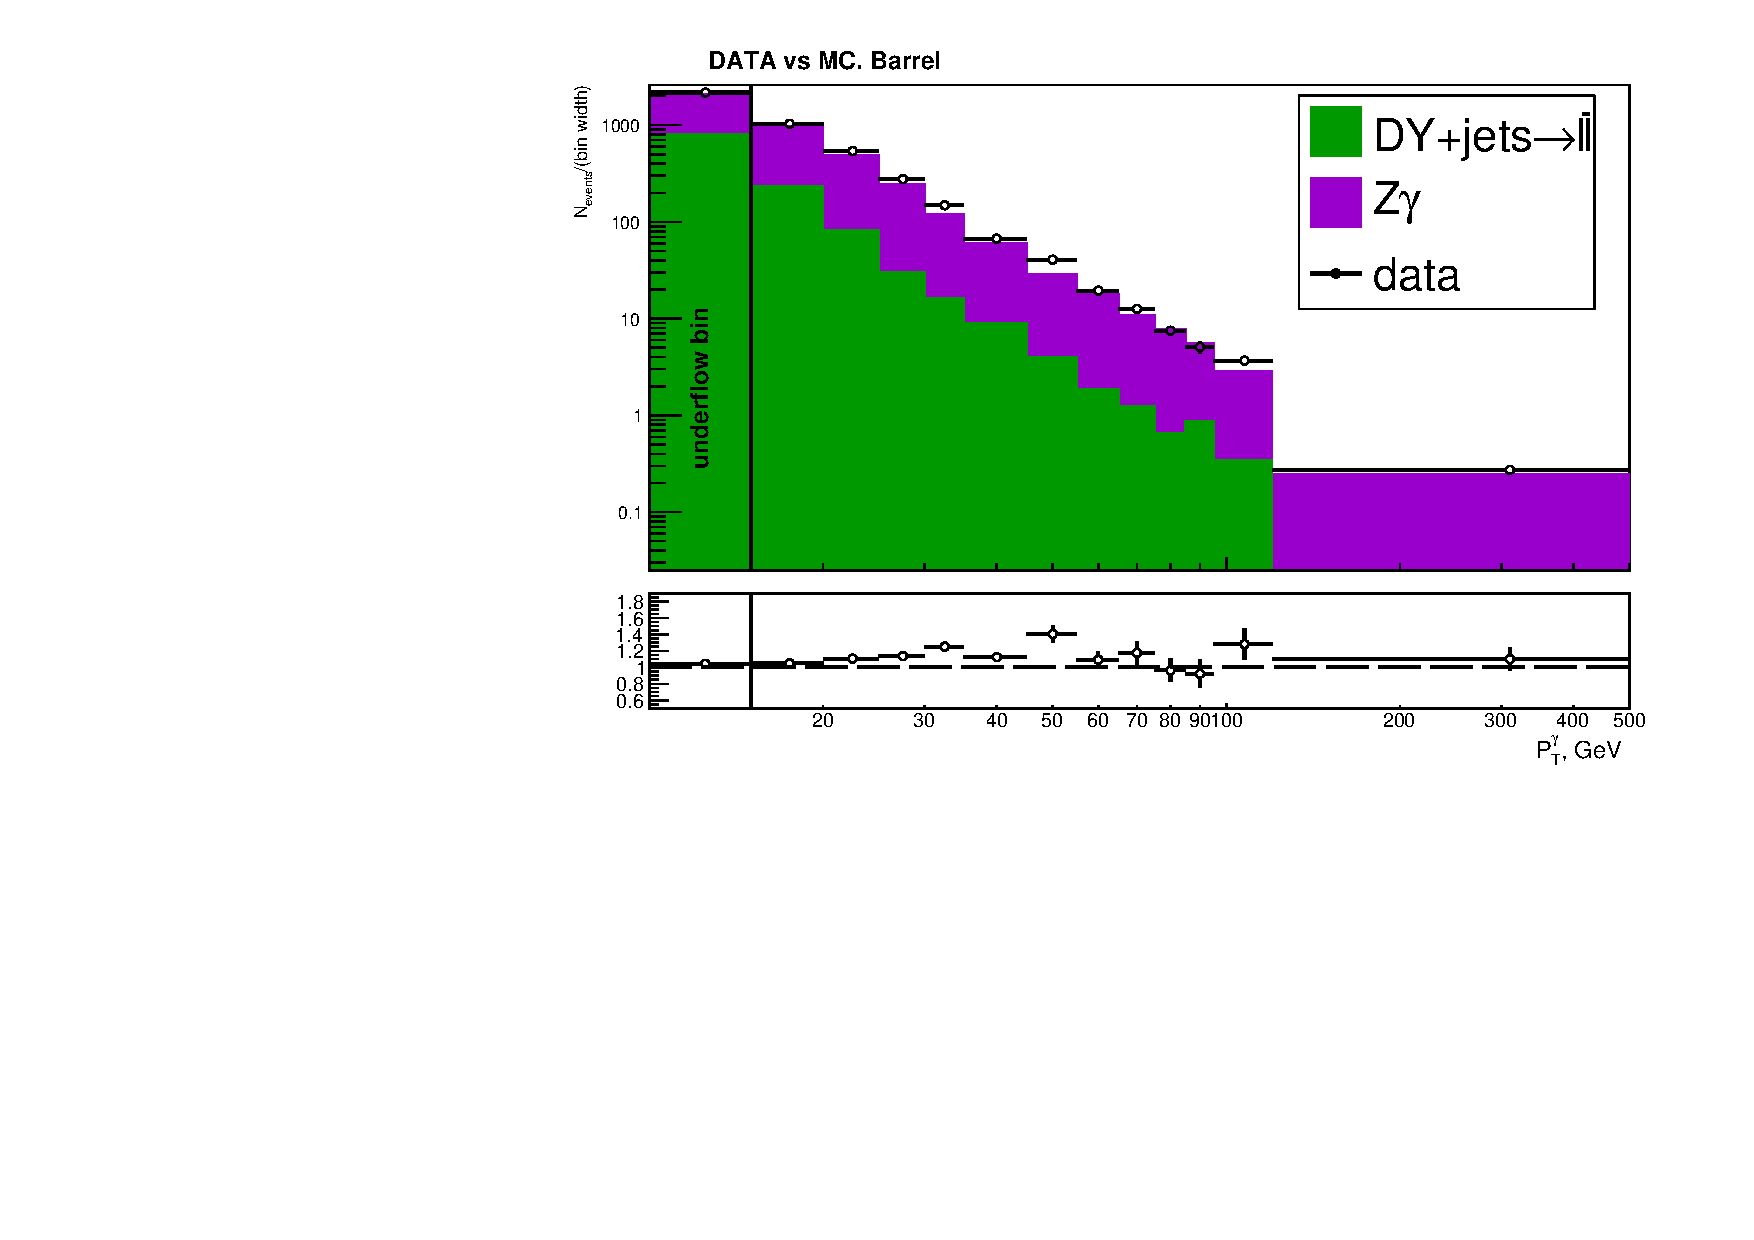
\includegraphics[width=0.45\textwidth]{../figs/figs_v11/ELECTRON_ZGamma/PrepareYields/c_TotalDATAvsMC_Barrel__phoEt.pdf}
   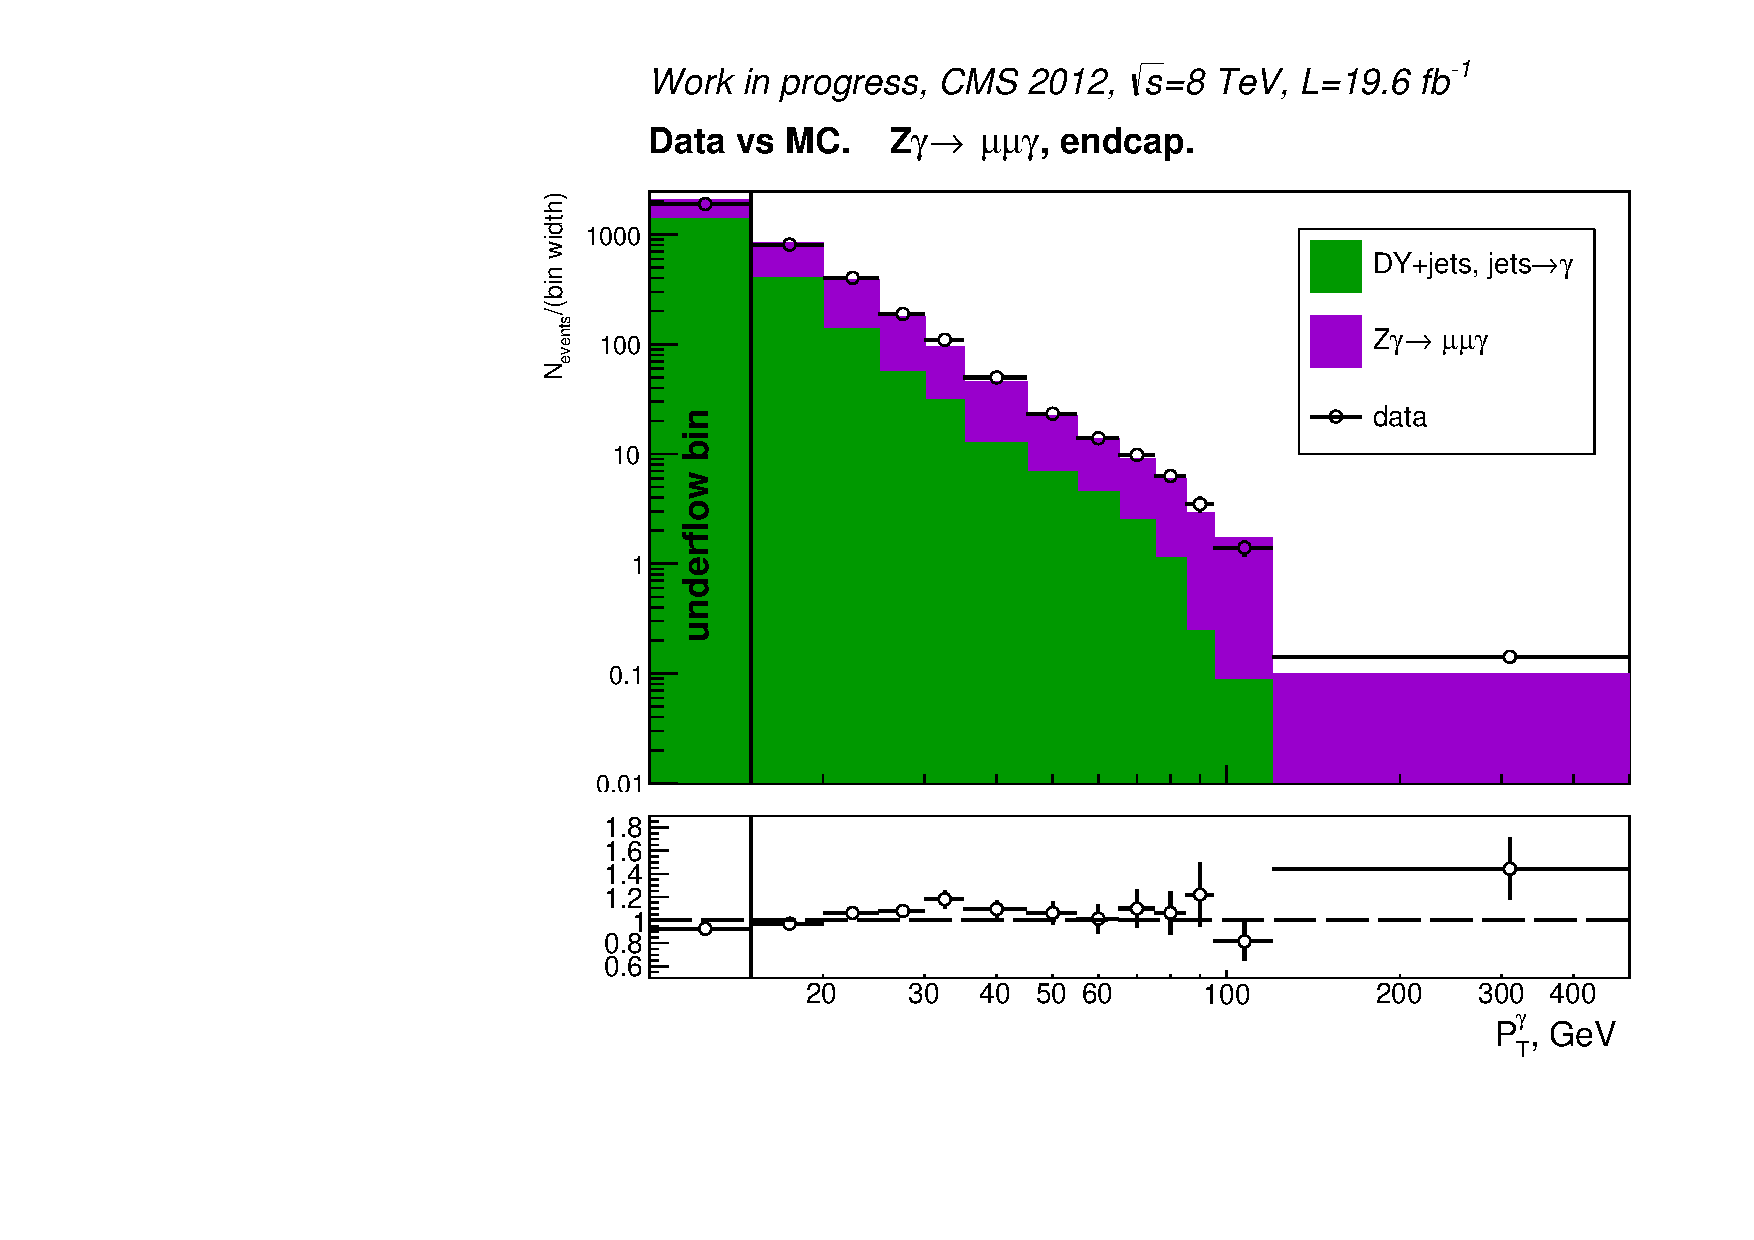
\includegraphics[width=0.45\textwidth]{../figs/figs_v11/MUON_ZGamma/PrepareYields/c_TotalDATAvsMC_Endcap__phoEt.pdf}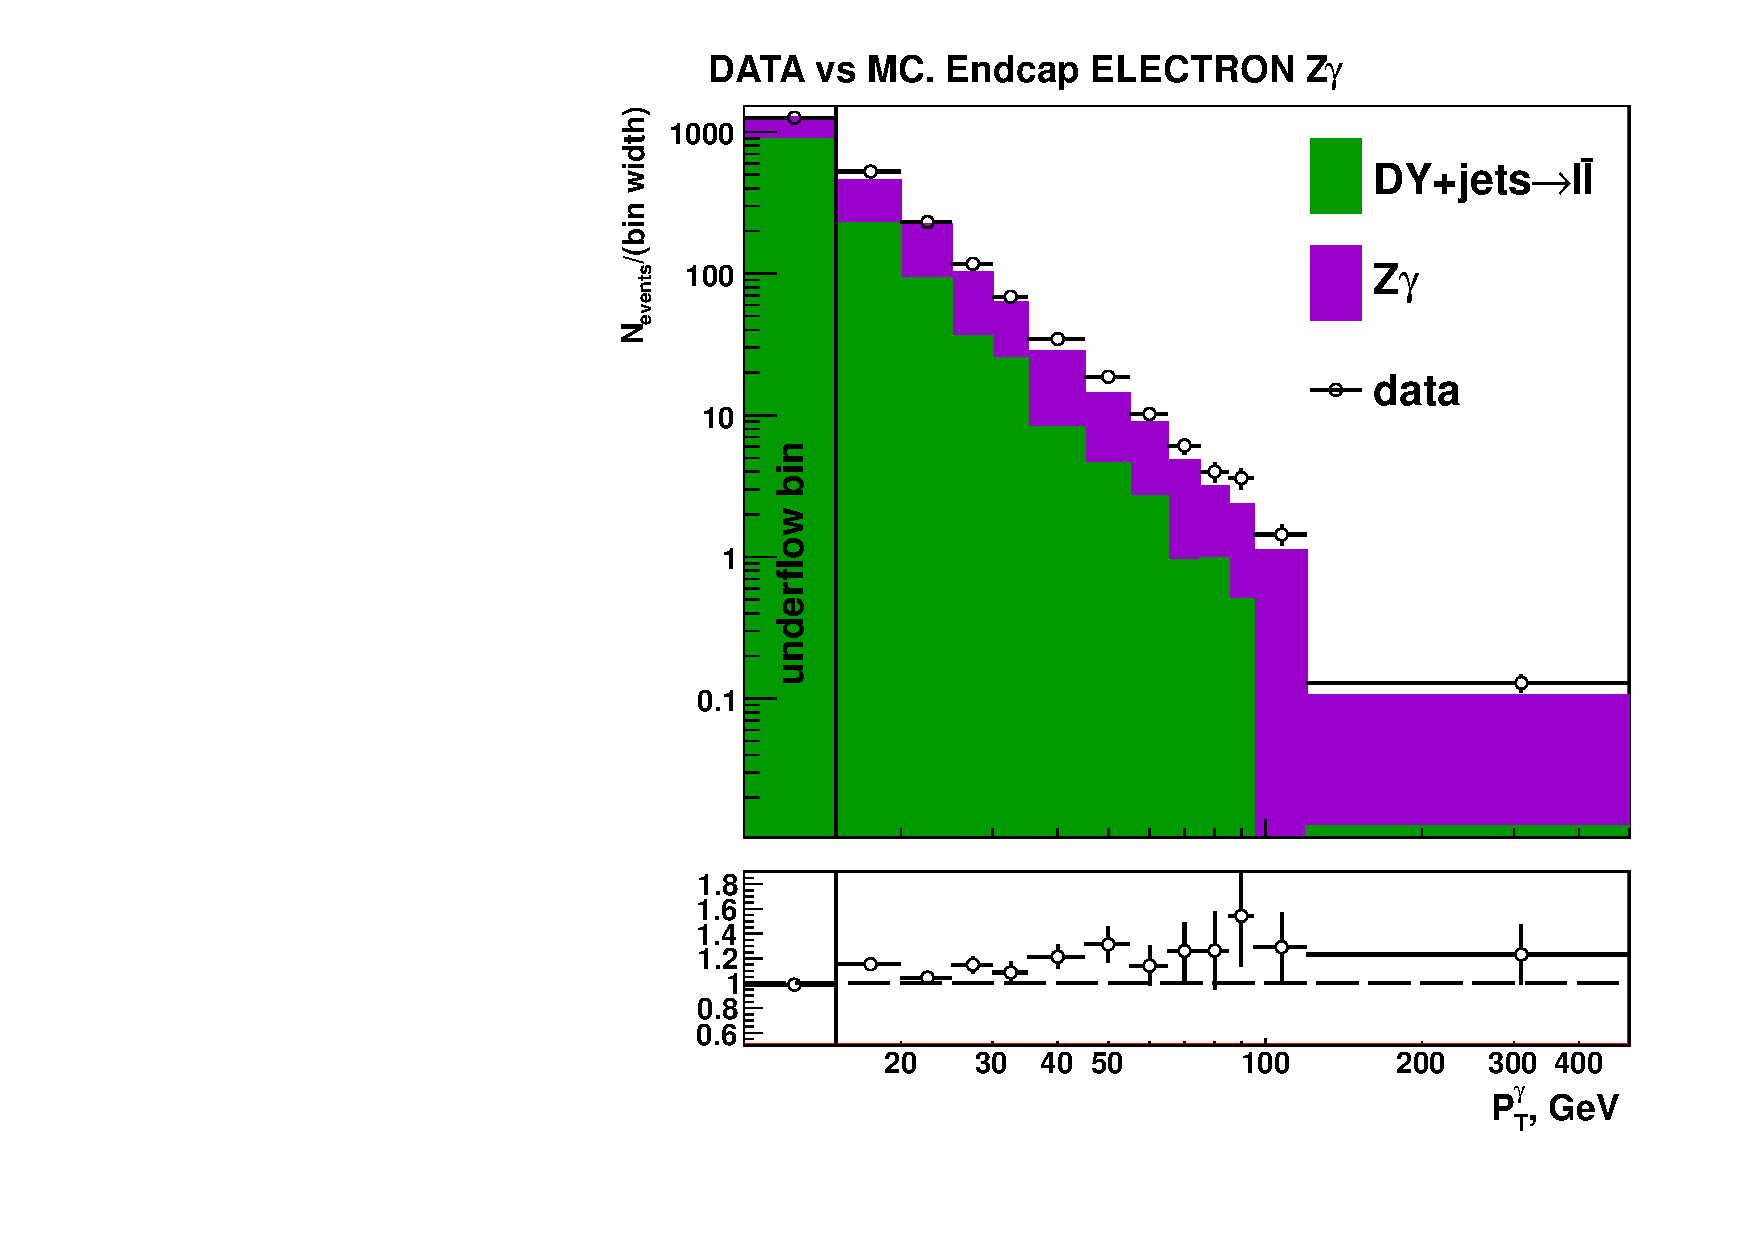
\includegraphics[width=0.45\textwidth]{../figs/figs_v11/ELECTRON_ZGamma/PrepareYields/c_TotalDATAvsMC_Endcap__phoEt.pdf}
  \caption{$P_T^{\gamma}$ distribution of $Z\gamma$ candidates in the muon (left) and electron (right) channels with photons in EB (top) and EE(bottom). Data vs total MC agreement is shown. The ratio plots are data divided by total MC.}
  \label{fig:DATAvsMC_Zg}
  \end{center}
\end{figure}

\begin{figure}[htb]
  \begin{center}
   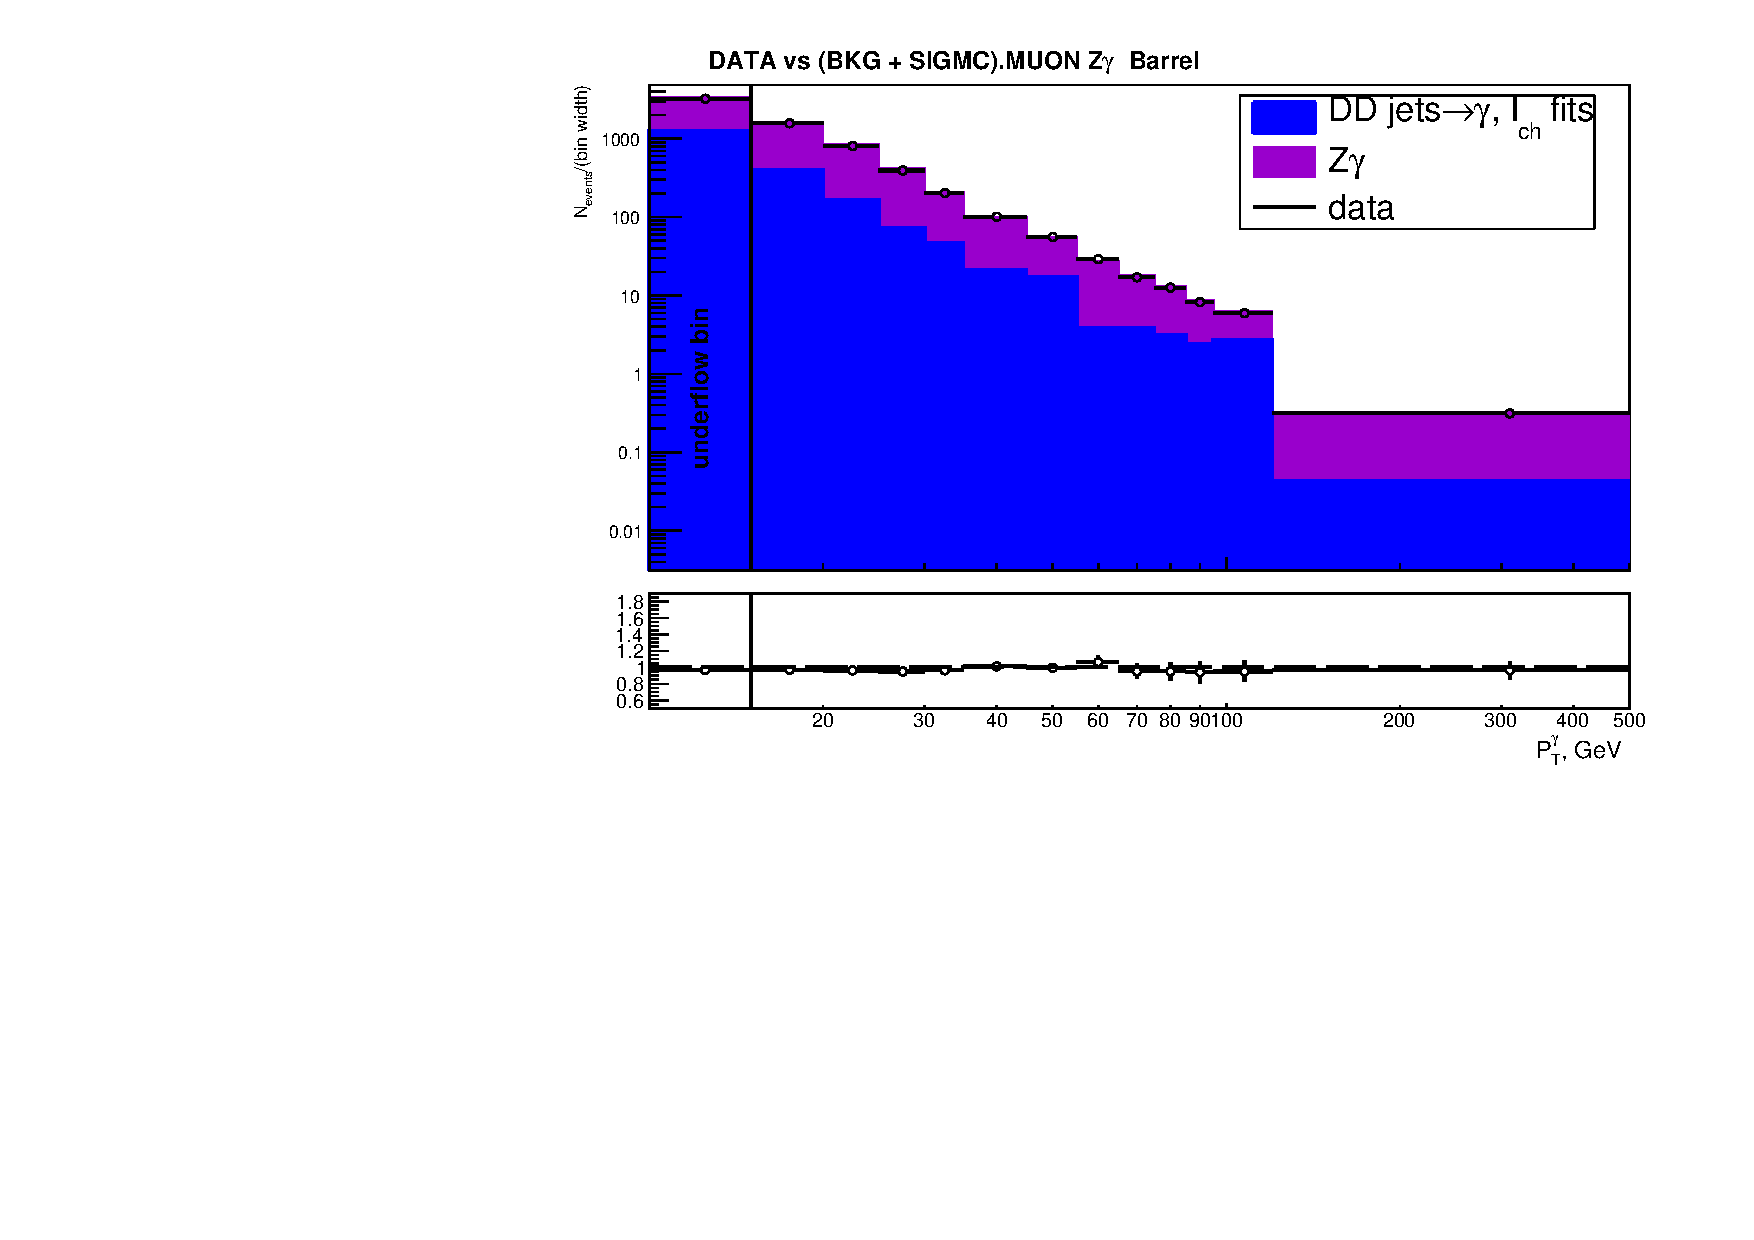
\includegraphics[width=0.45\textwidth]{../figs/figs_v11/MUON_ZGamma/PrepareYields/c_DATAvsBkgPlusSigMCc_MUON_ZGamma_TEMPL_CHISO_UNblind__Barrel__phoEt.pdf}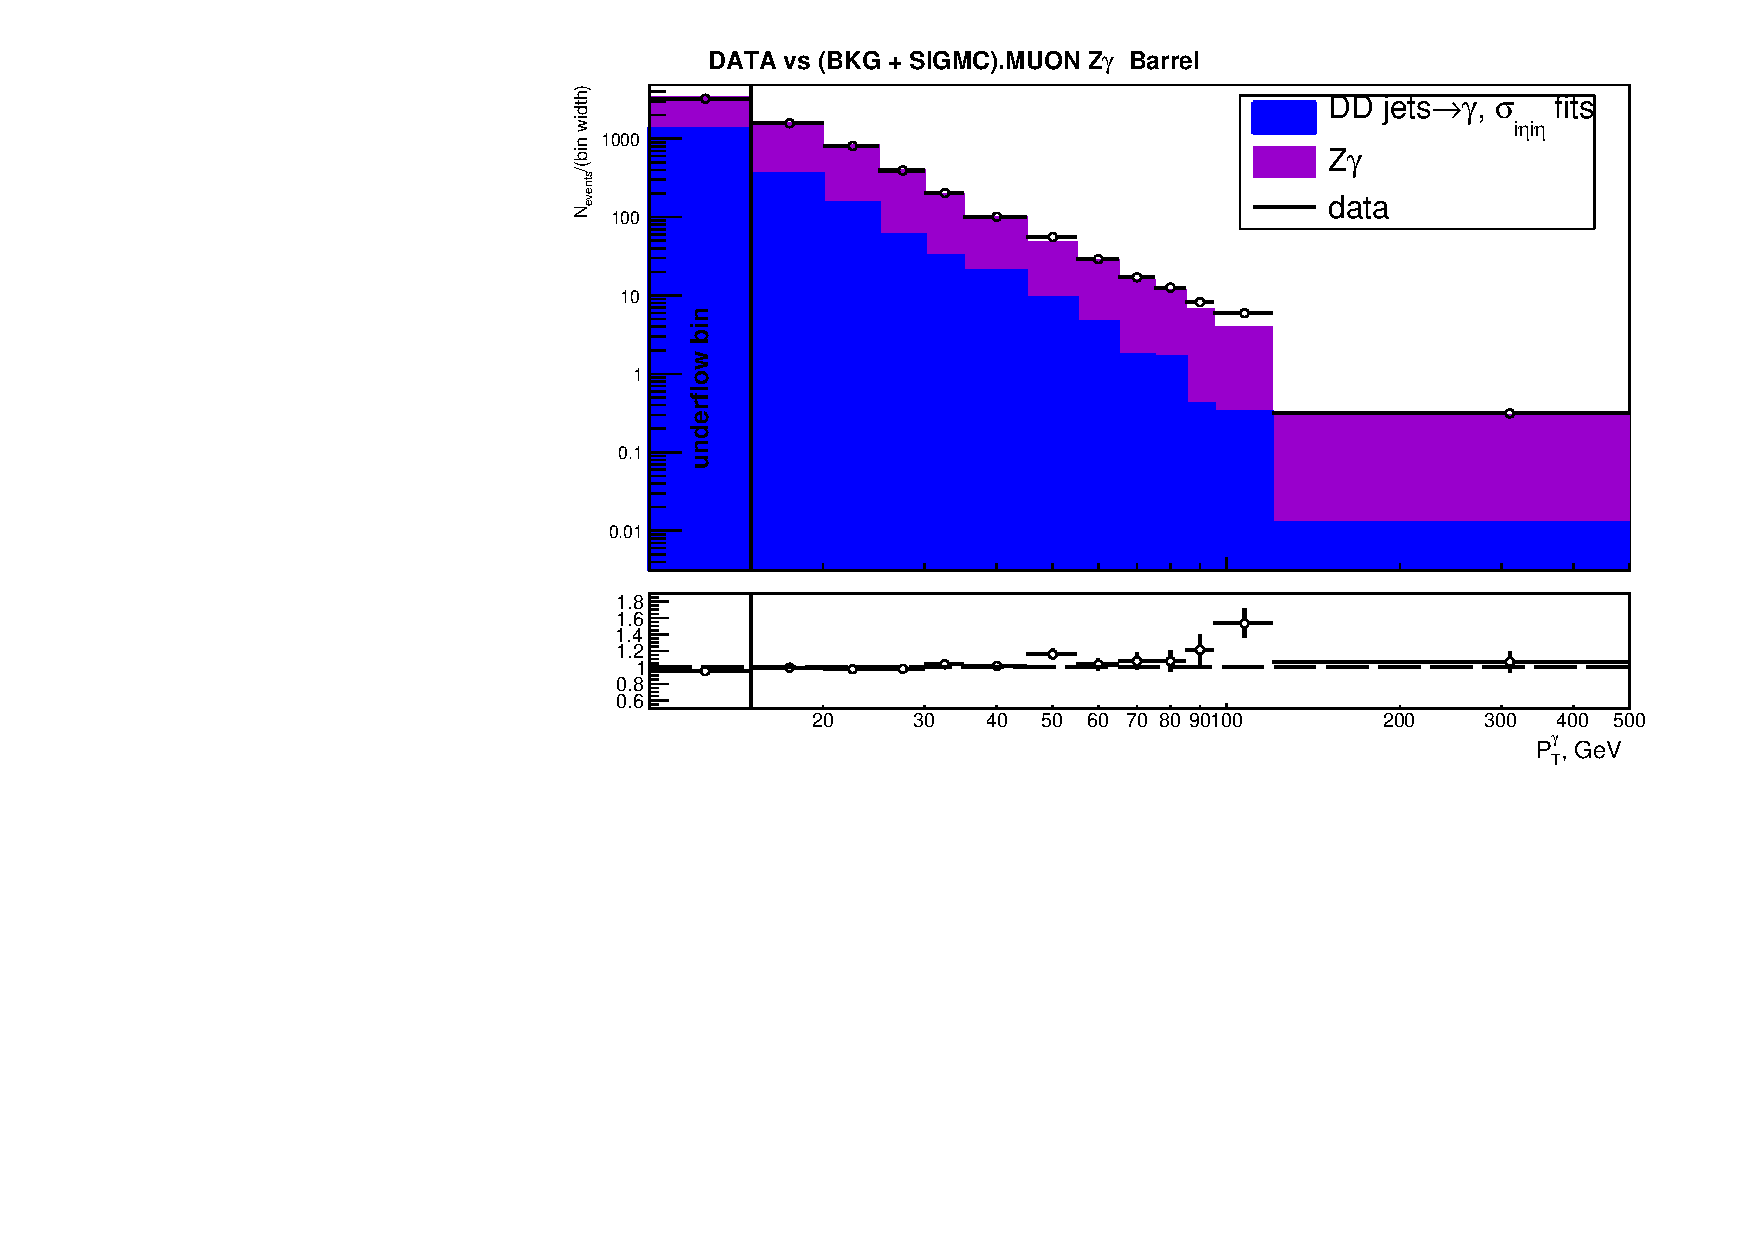
\includegraphics[width=0.45\textwidth]{../figs/figs_v11/MUON_ZGamma/PrepareYields/c_DATAvsBkgPlusSigMCc_MUON_ZGamma_TEMPL_SIHIH_UNblind__Barrel__phoEt.pdf}  \\
   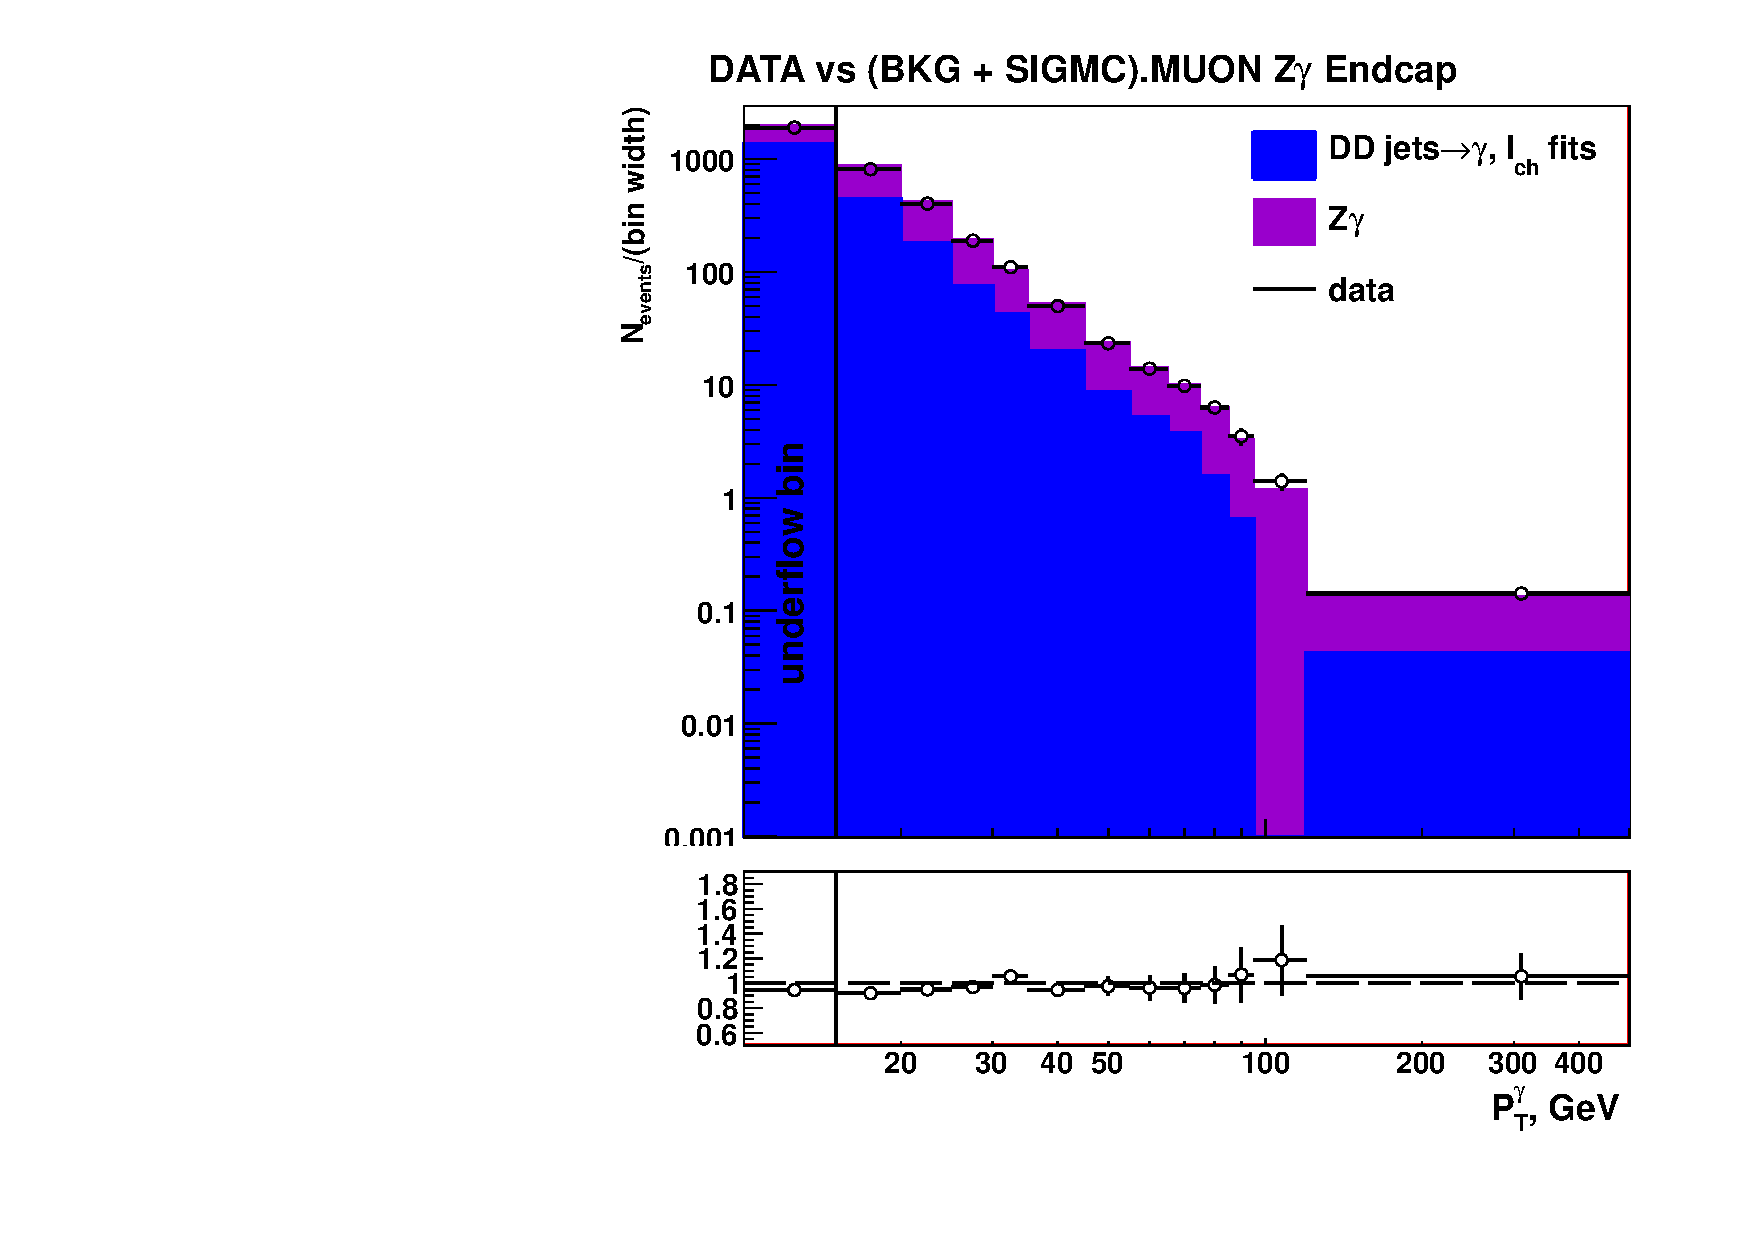
\includegraphics[width=0.45\textwidth]{../figs/figs_v11/MUON_ZGamma/PrepareYields/c_DATAvsBkgPlusSigMCc_MUON_ZGamma_TEMPL_CHISO_UNblind__Endcap__phoEt.pdf}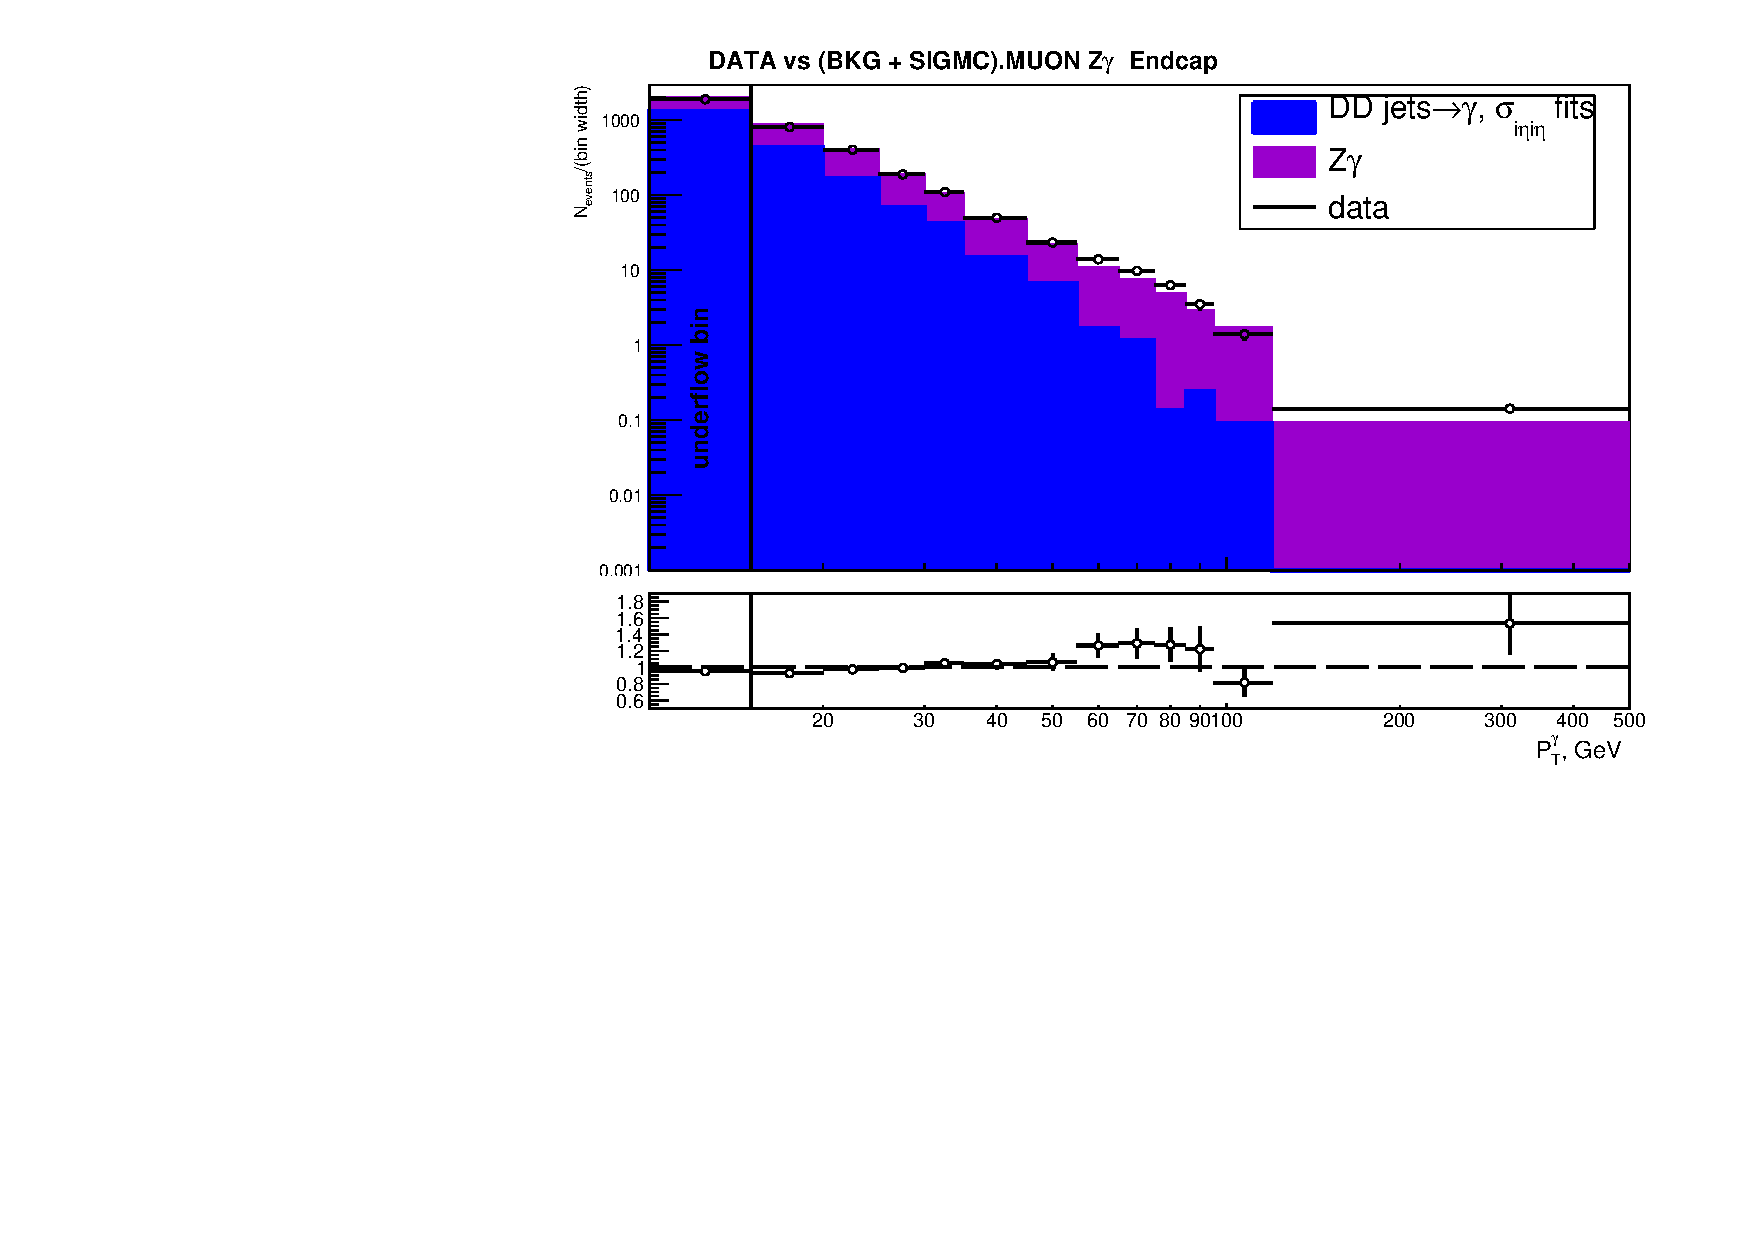
\includegraphics[width=0.45\textwidth]{../figs/figs_v11/MUON_ZGamma/PrepareYields/c_DATAvsBkgPlusSigMCc_MUON_ZGamma_TEMPL_SIHIH_UNblind__Endcap__phoEt.pdf}  \\
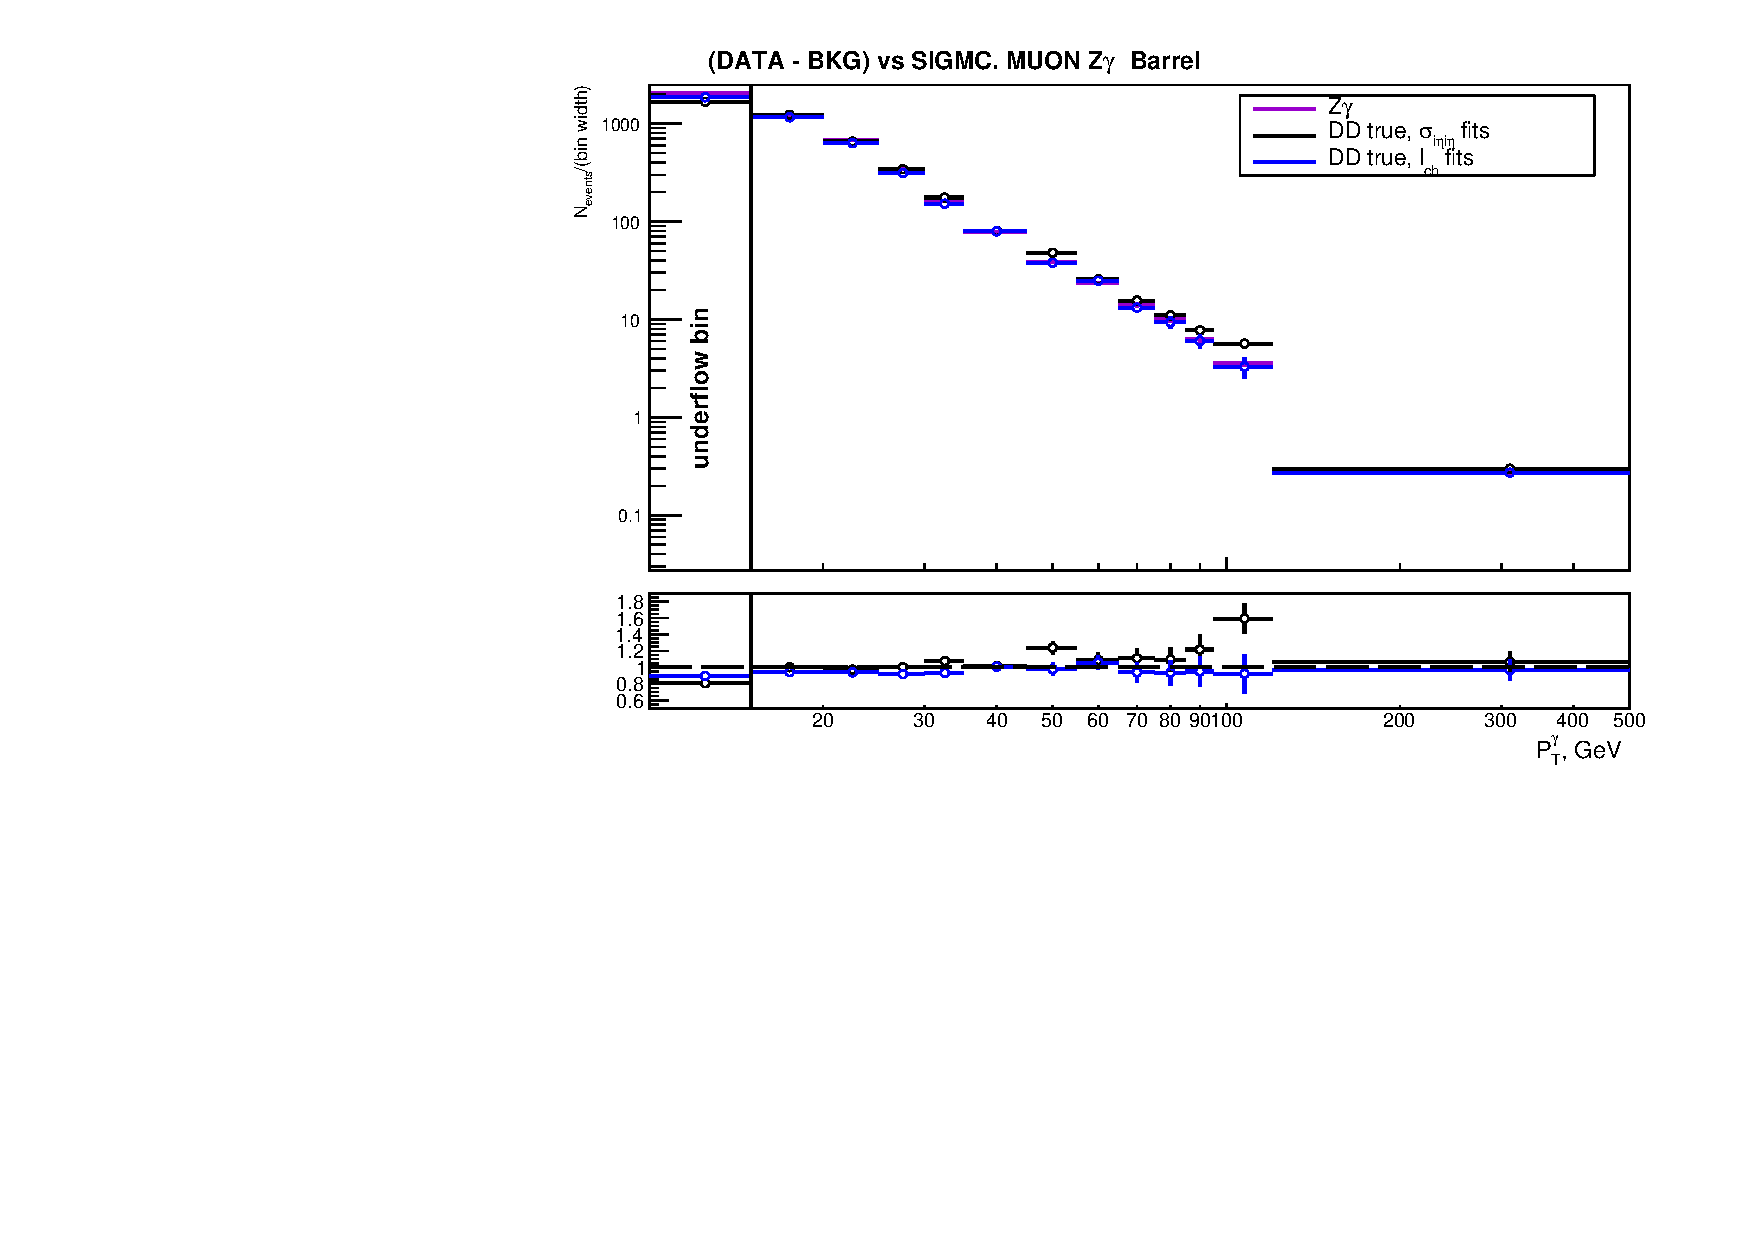
\includegraphics[width=0.45\textwidth]{../figs/figs_v11/MUON_ZGamma/PrepareYields/c_BkgSubtrDATAvsSIGMC_c_MUON_ZGamma__UNblind__Barrel__phoEt.pdf}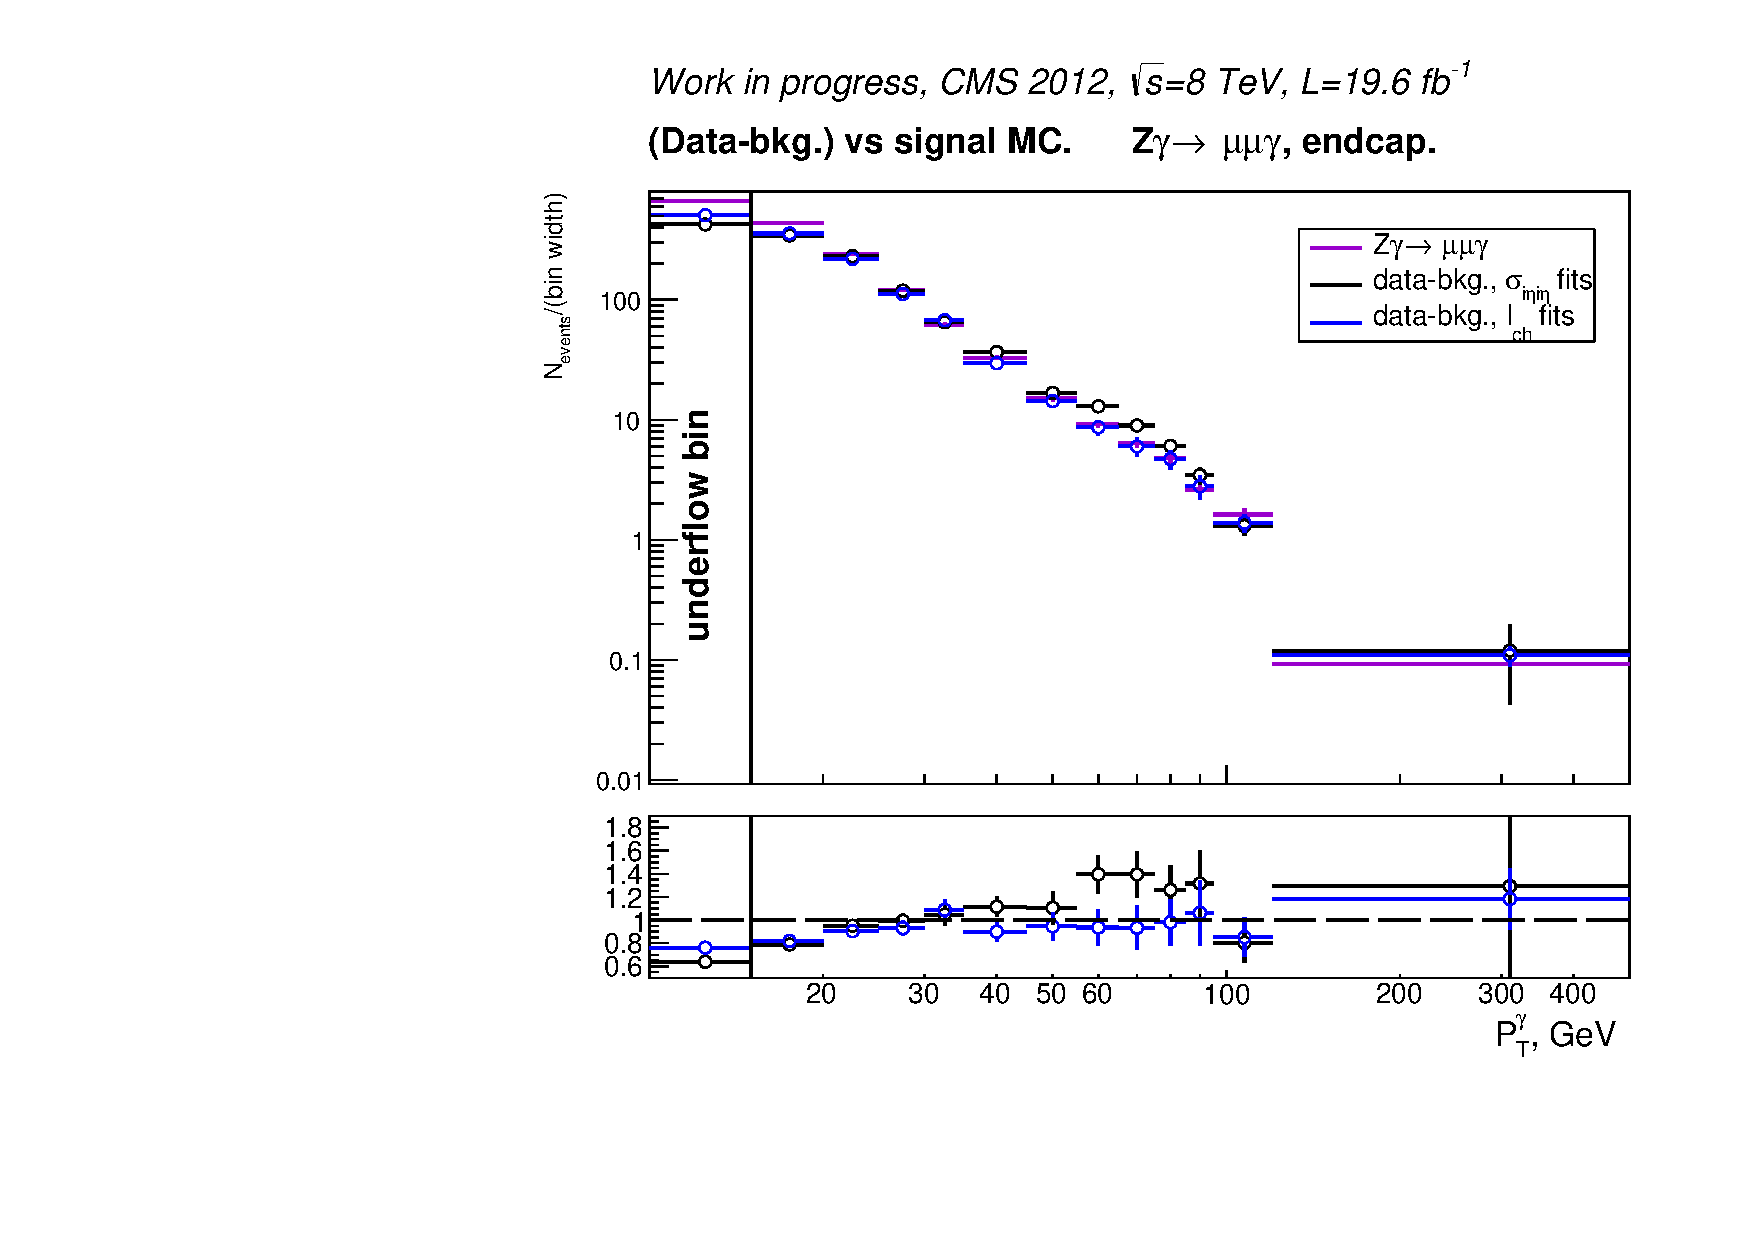
\includegraphics[width=0.45\textwidth]{../figs/figs_v11/MUON_ZGamma/PrepareYields/c_BkgSubtrDATAvsSIGMC_c_MUON_ZGamma__UNblind__Endcap__phoEt.pdf}\\
  \caption{$P_T^{\gamma}$ distribution of $Z\gamma$ candidates in the muon channel. Top and middle: data vs fake-$\gamma$ background derived from the template method + real-$\gamma$ background predicted by dedicated MC samples + signal MC, with $I_{ch}$ (left) and $\sigma_{i\eta i\eta}$ (right) used as fit variables for candidates with photons in EB (top) and EE (middle). Bottom: data yields after full background subtraction vs signal MC for candidates with photons in in EB (left) and EE (right).}
  \label{fig:DDvsMC_Zg_Data_MUON}
  \end{center}
\end{figure}

\begin{figure}[htb]
  \begin{center}
   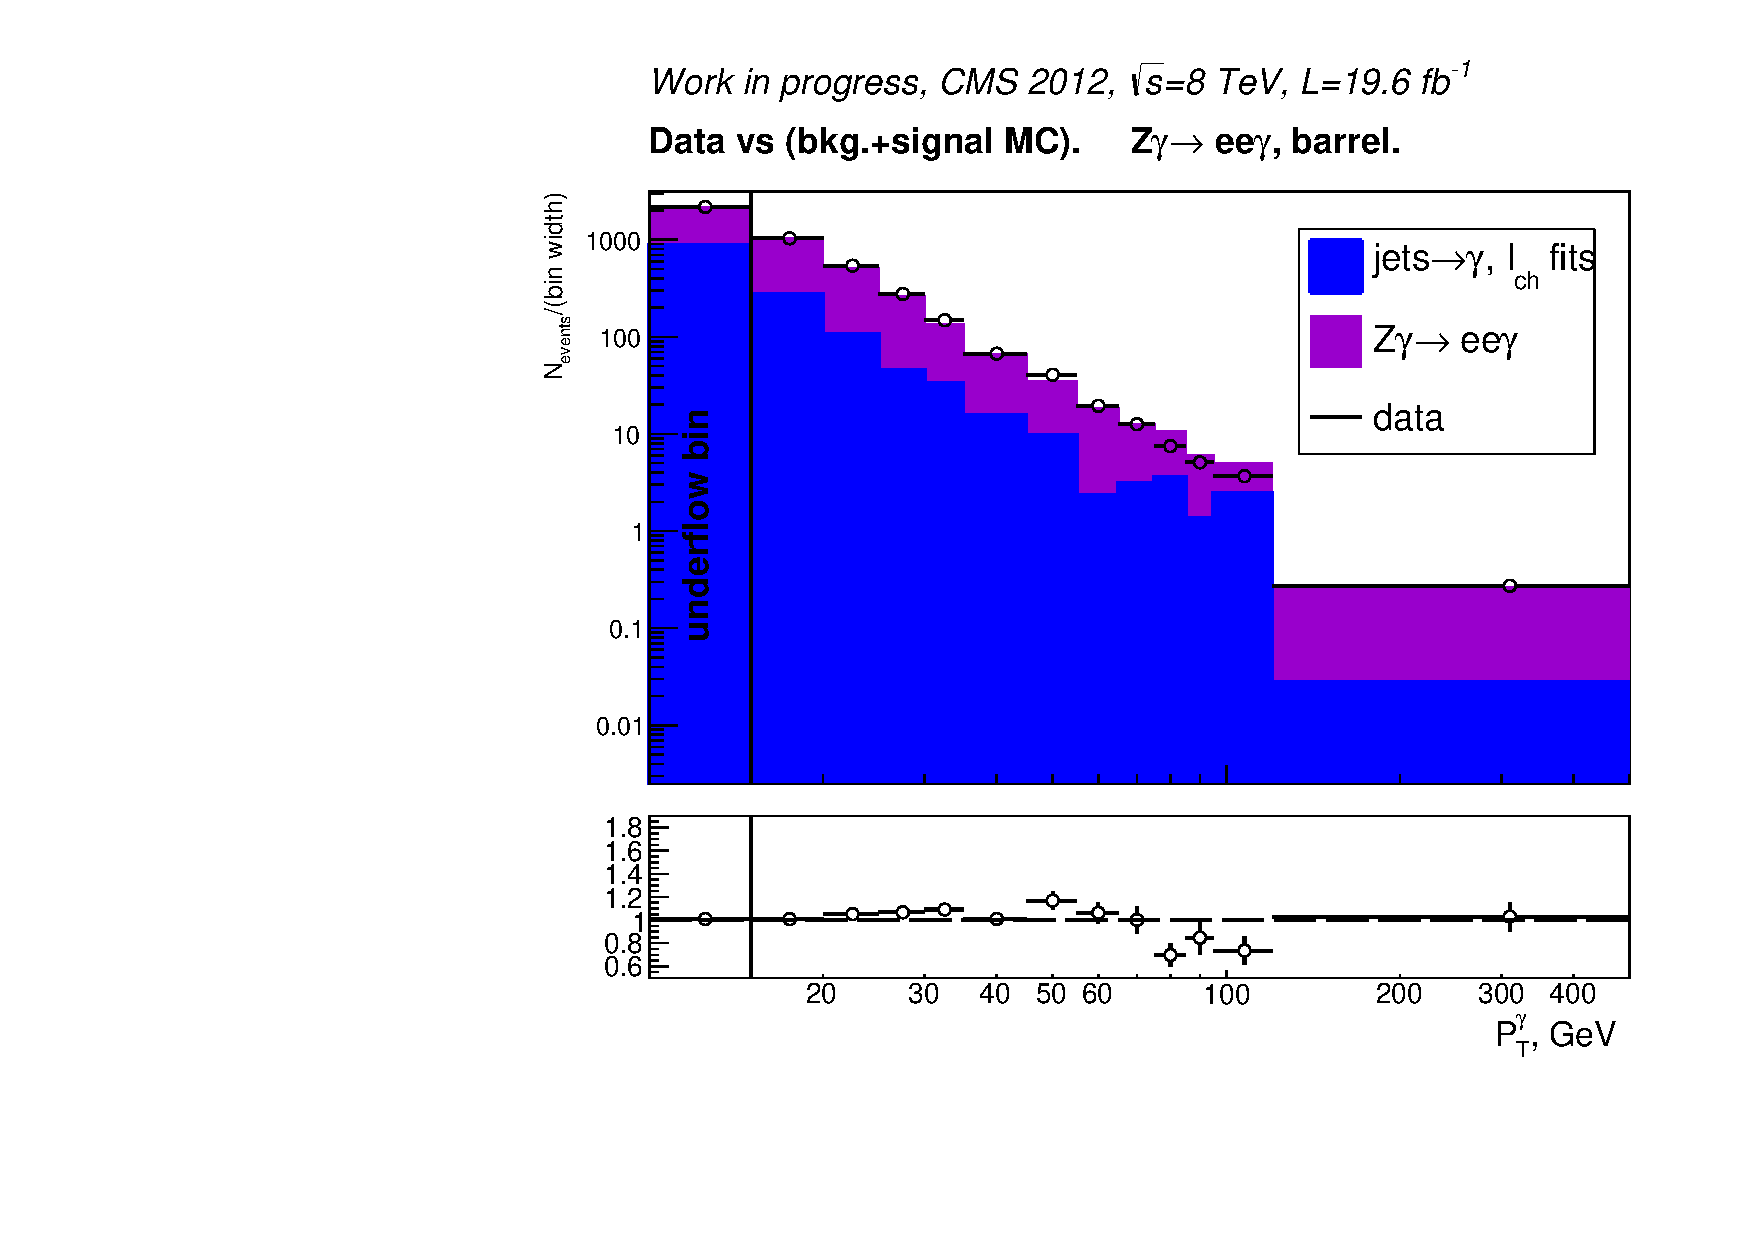
\includegraphics[width=0.45\textwidth]{../figs/figs_v11/ELECTRON_ZGamma/PrepareYields/c_DATAvsBkgPlusSigMCc_ELECTRON_ZGamma_TEMPL_CHISO_UNblind__Barrel__phoEt.pdf}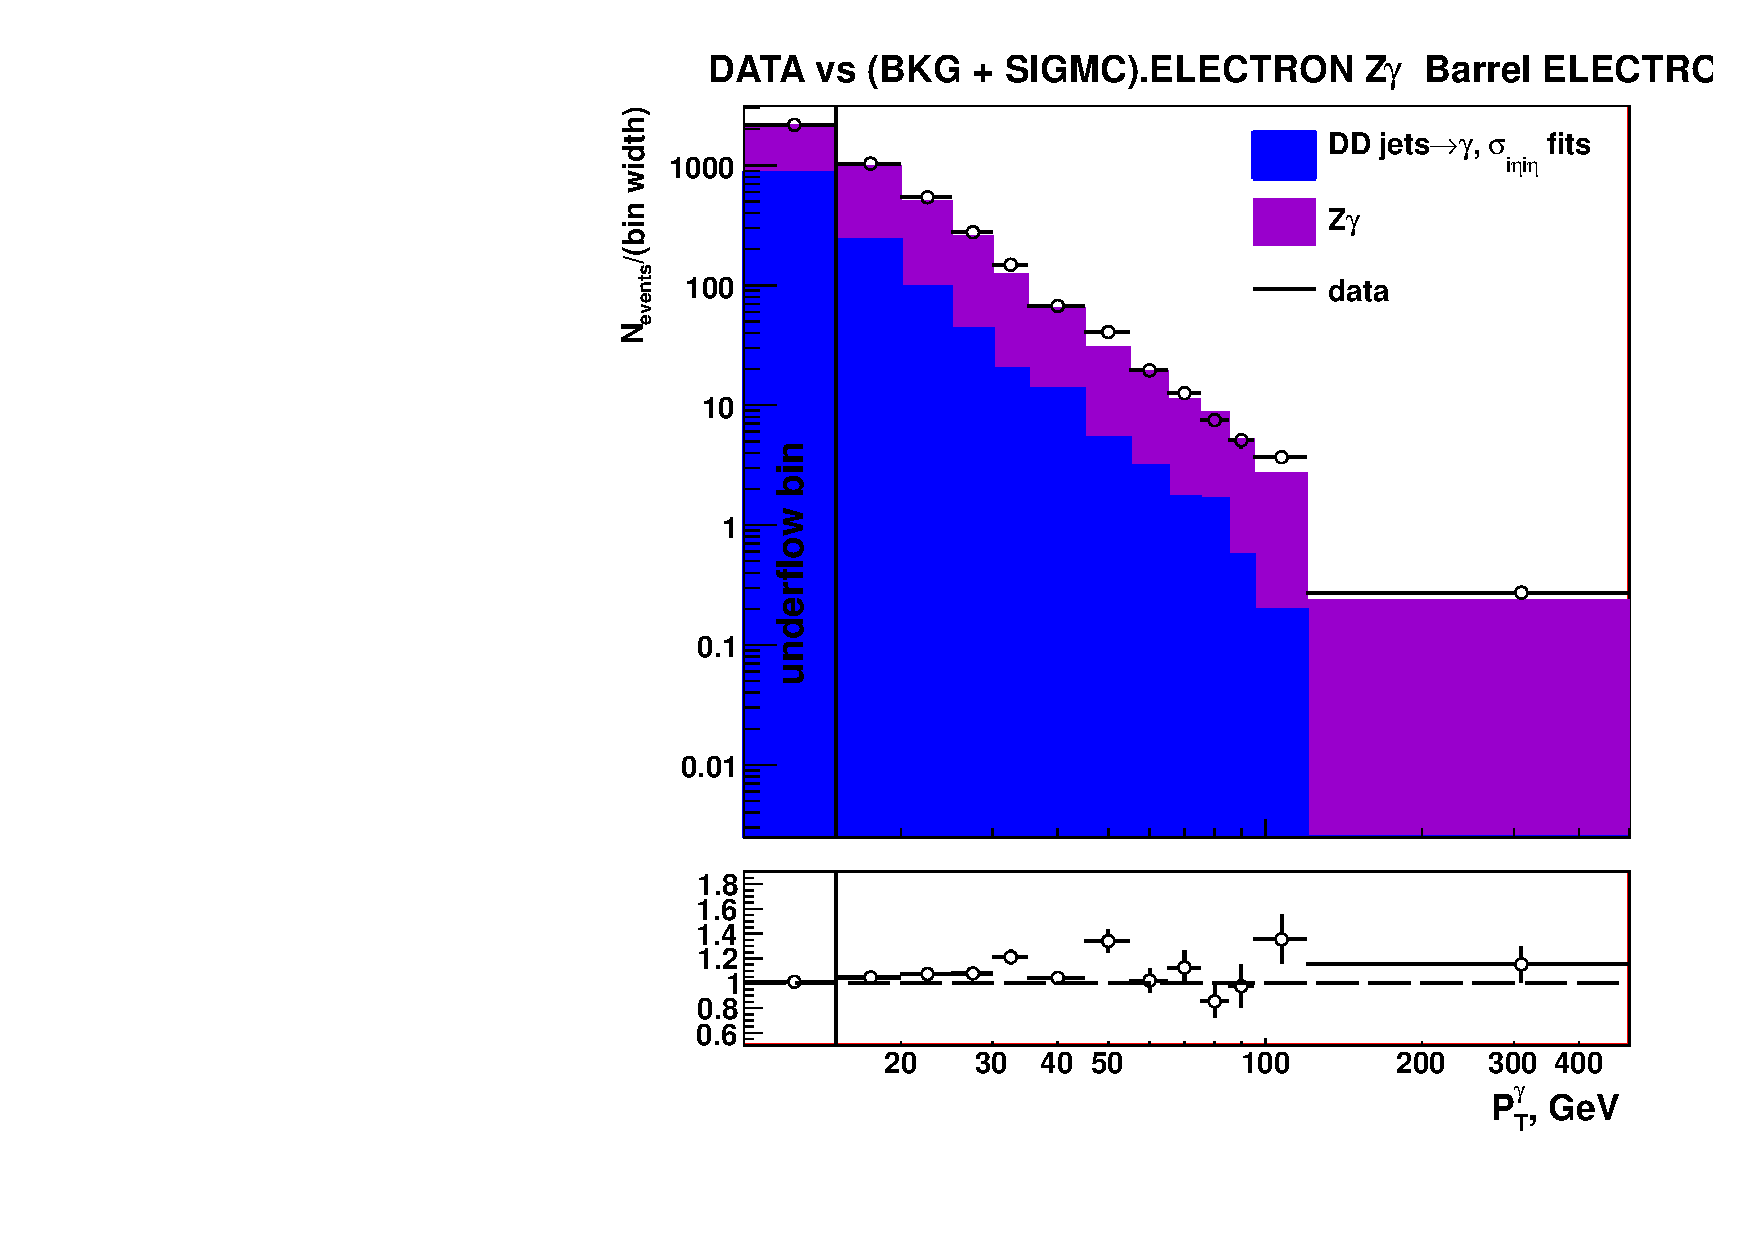
\includegraphics[width=0.45\textwidth]{../figs/figs_v11/ELECTRON_ZGamma/PrepareYields/c_DATAvsBkgPlusSigMCc_ELECTRON_ZGamma_TEMPL_SIHIH_UNblind__Barrel__phoEt.pdf}  \\
   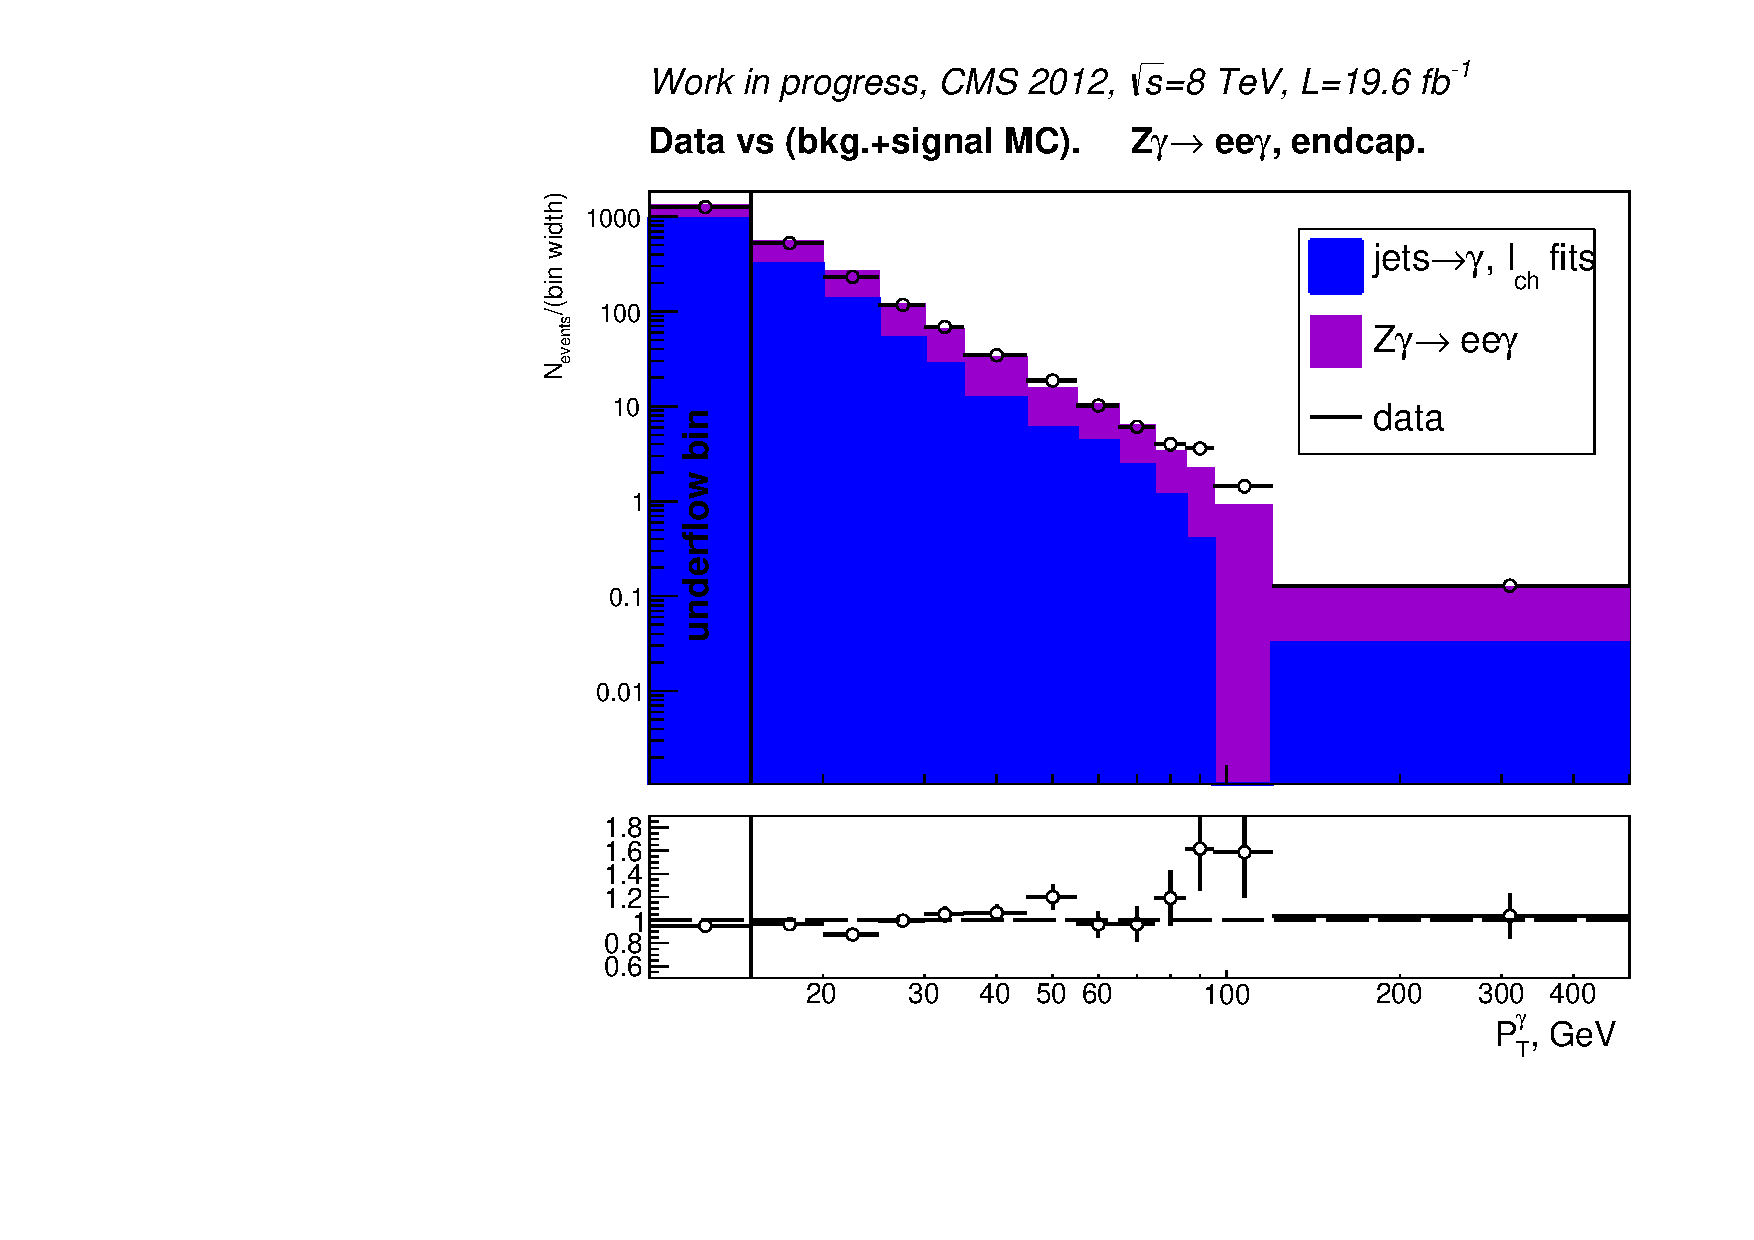
\includegraphics[width=0.45\textwidth]{../figs/figs_v11/ELECTRON_ZGamma/PrepareYields/c_DATAvsBkgPlusSigMCc_ELECTRON_ZGamma_TEMPL_CHISO_UNblind__Endcap__phoEt.pdf}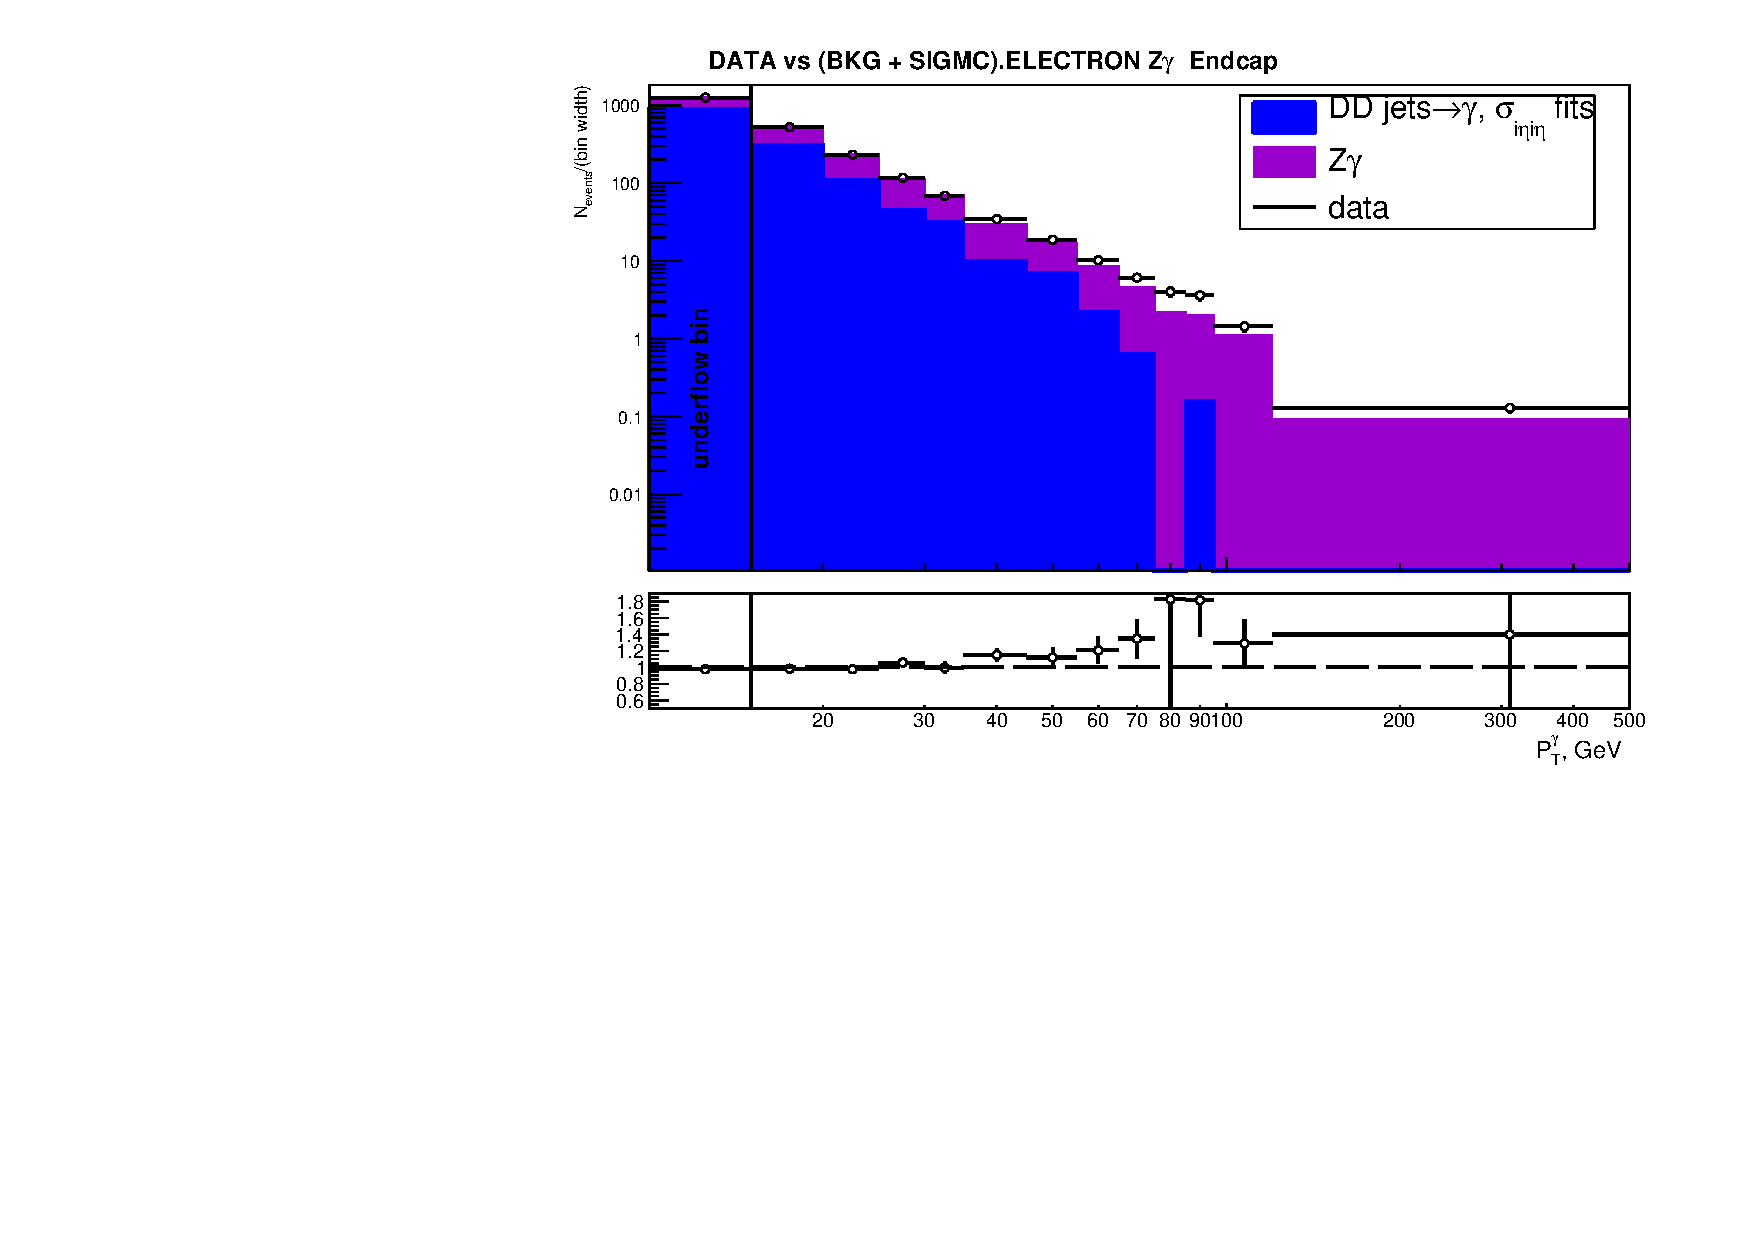
\includegraphics[width=0.45\textwidth]{../figs/figs_v11/ELECTRON_ZGamma/PrepareYields/c_DATAvsBkgPlusSigMCc_ELECTRON_ZGamma_TEMPL_SIHIH_UNblind__Endcap__phoEt.pdf}  \\
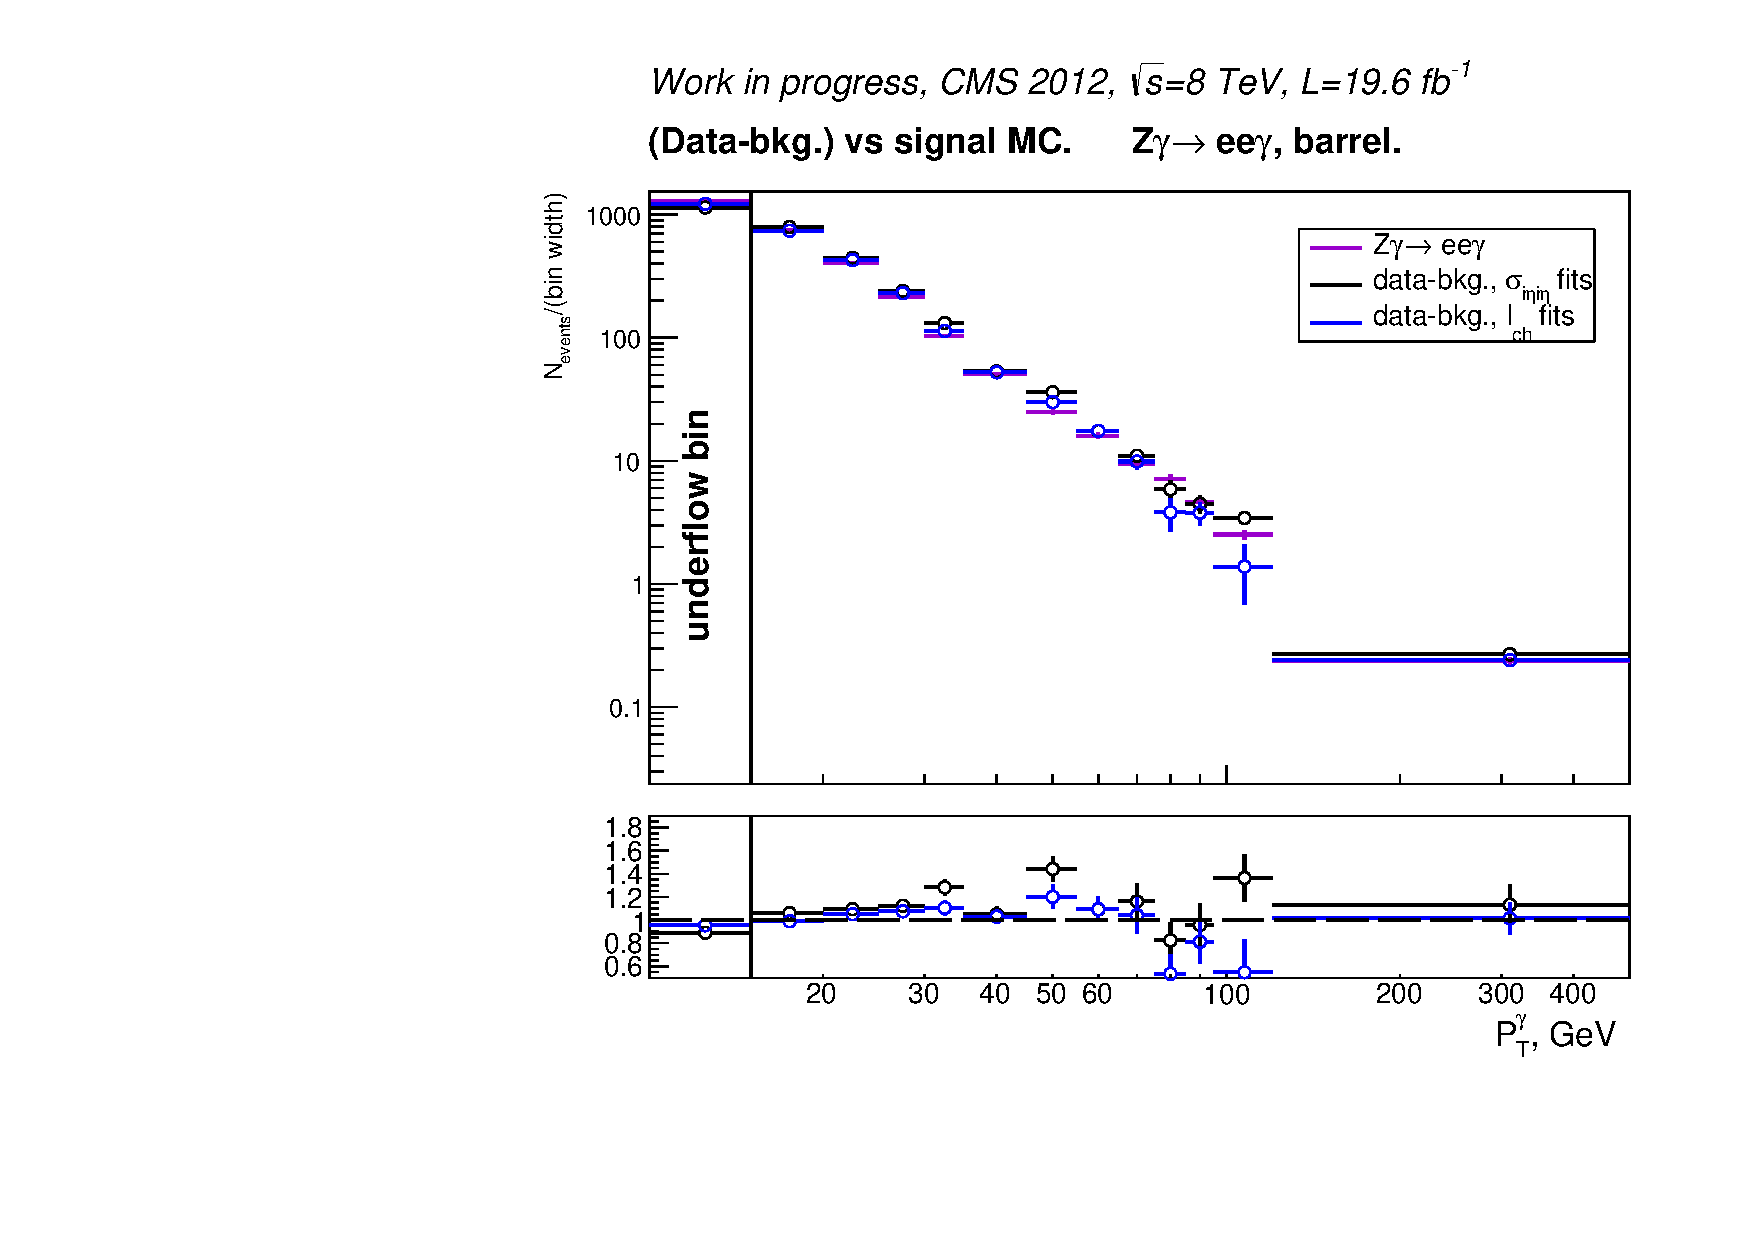
\includegraphics[width=0.45\textwidth]{../figs/figs_v11/ELECTRON_ZGamma/PrepareYields/c_BkgSubtrDATAvsSIGMC_c_ELECTRON_ZGamma__UNblind__Barrel__phoEt.pdf}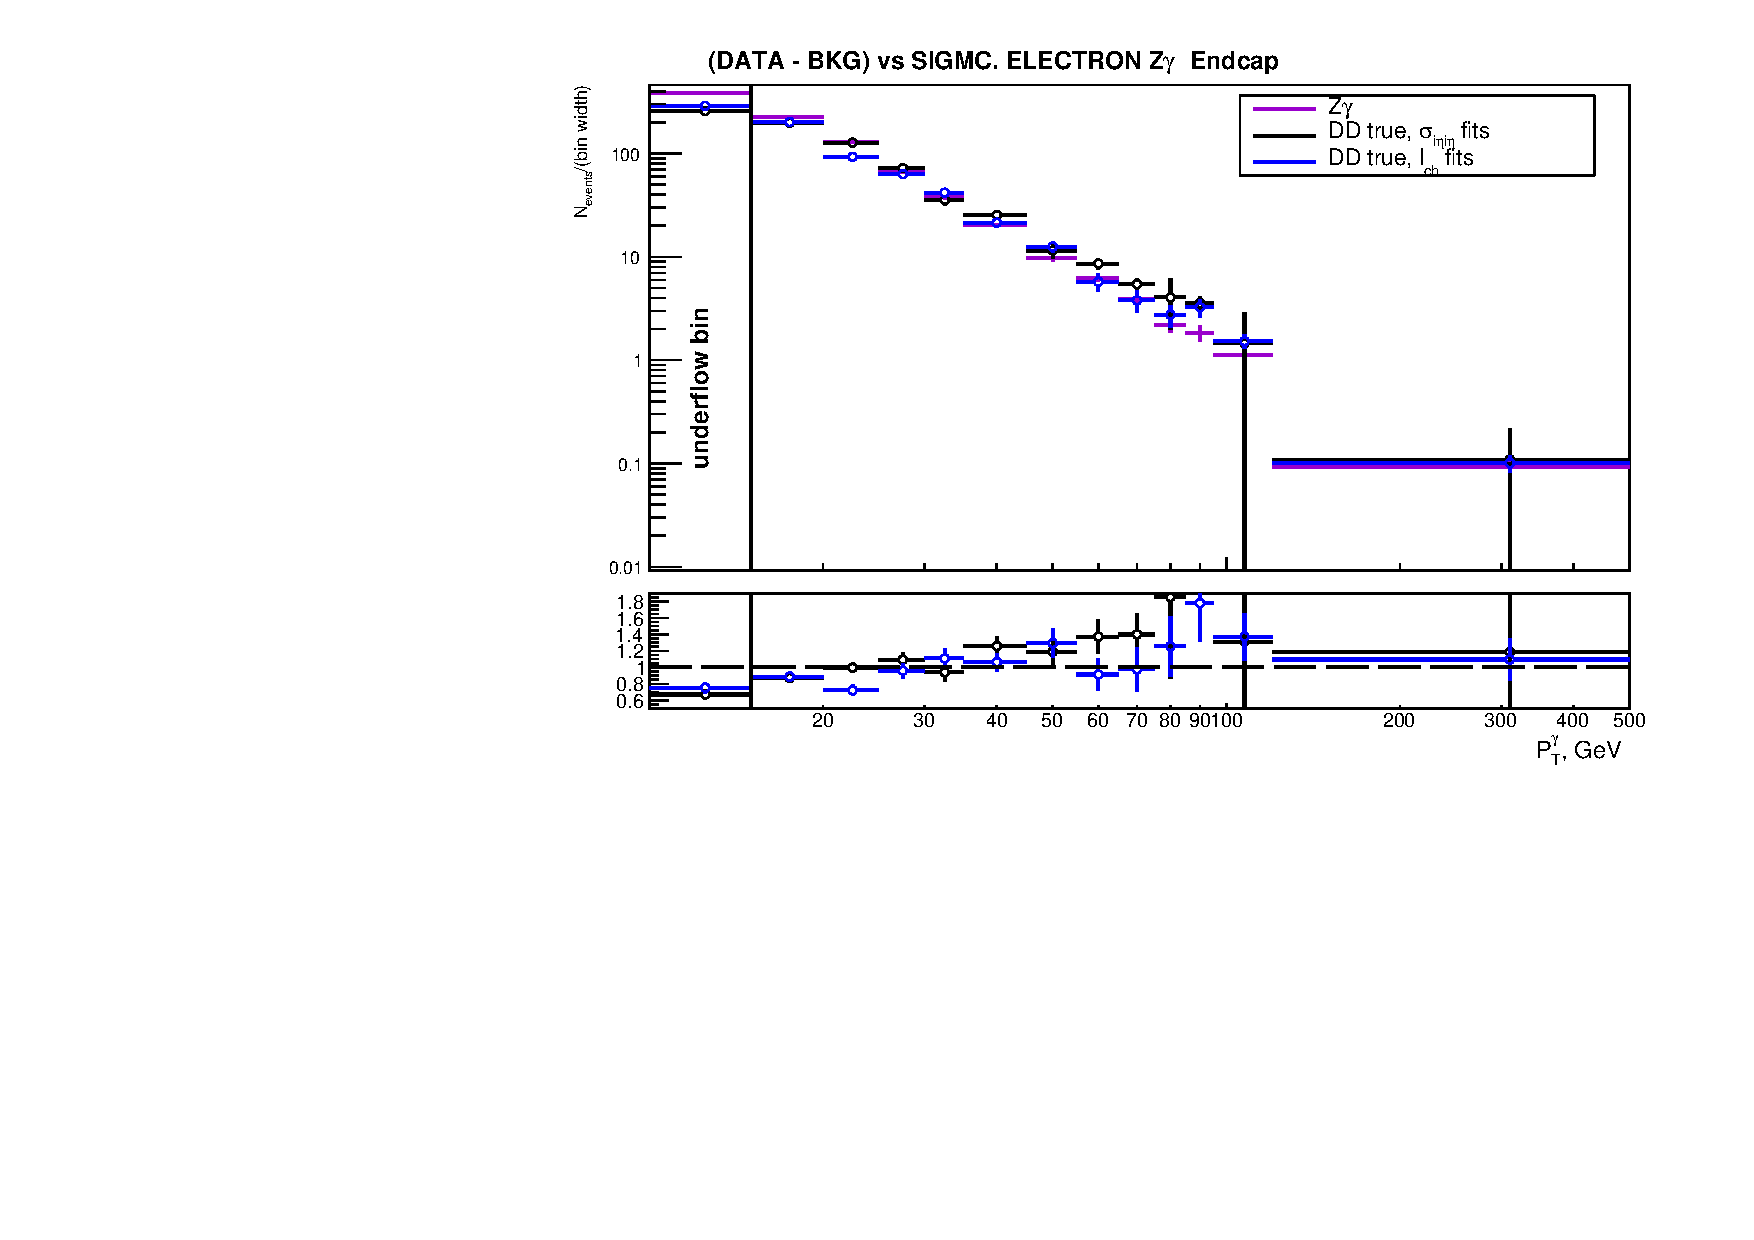
\includegraphics[width=0.45\textwidth]{../figs/figs_v11/ELECTRON_ZGamma/PrepareYields/c_BkgSubtrDATAvsSIGMC_c_ELECTRON_ZGamma__UNblind__Endcap__phoEt.pdf}\\
  \caption{$P_T^{\gamma}$ distribution of $Z\gamma$ candidates in the electron channel. Top and middle: data vs fake-$\gamma$ background derived from the template method + real-$\gamma$ background predicted by dedicated MC samples + signal MC, with $I_{ch}$ (left) and $\sigma_{i\eta i\eta}$ (right) used as fit variables in EB (top) and EE (middle). Bottom: data yields after full background subtraction vs signal MC in EB (left) and EE (right).}
  \label{fig:DDvsMC_Zg_Data_ELECTRON}
  \end{center}
\end{figure}

\begin{figure}[htb]
  \begin{center}
   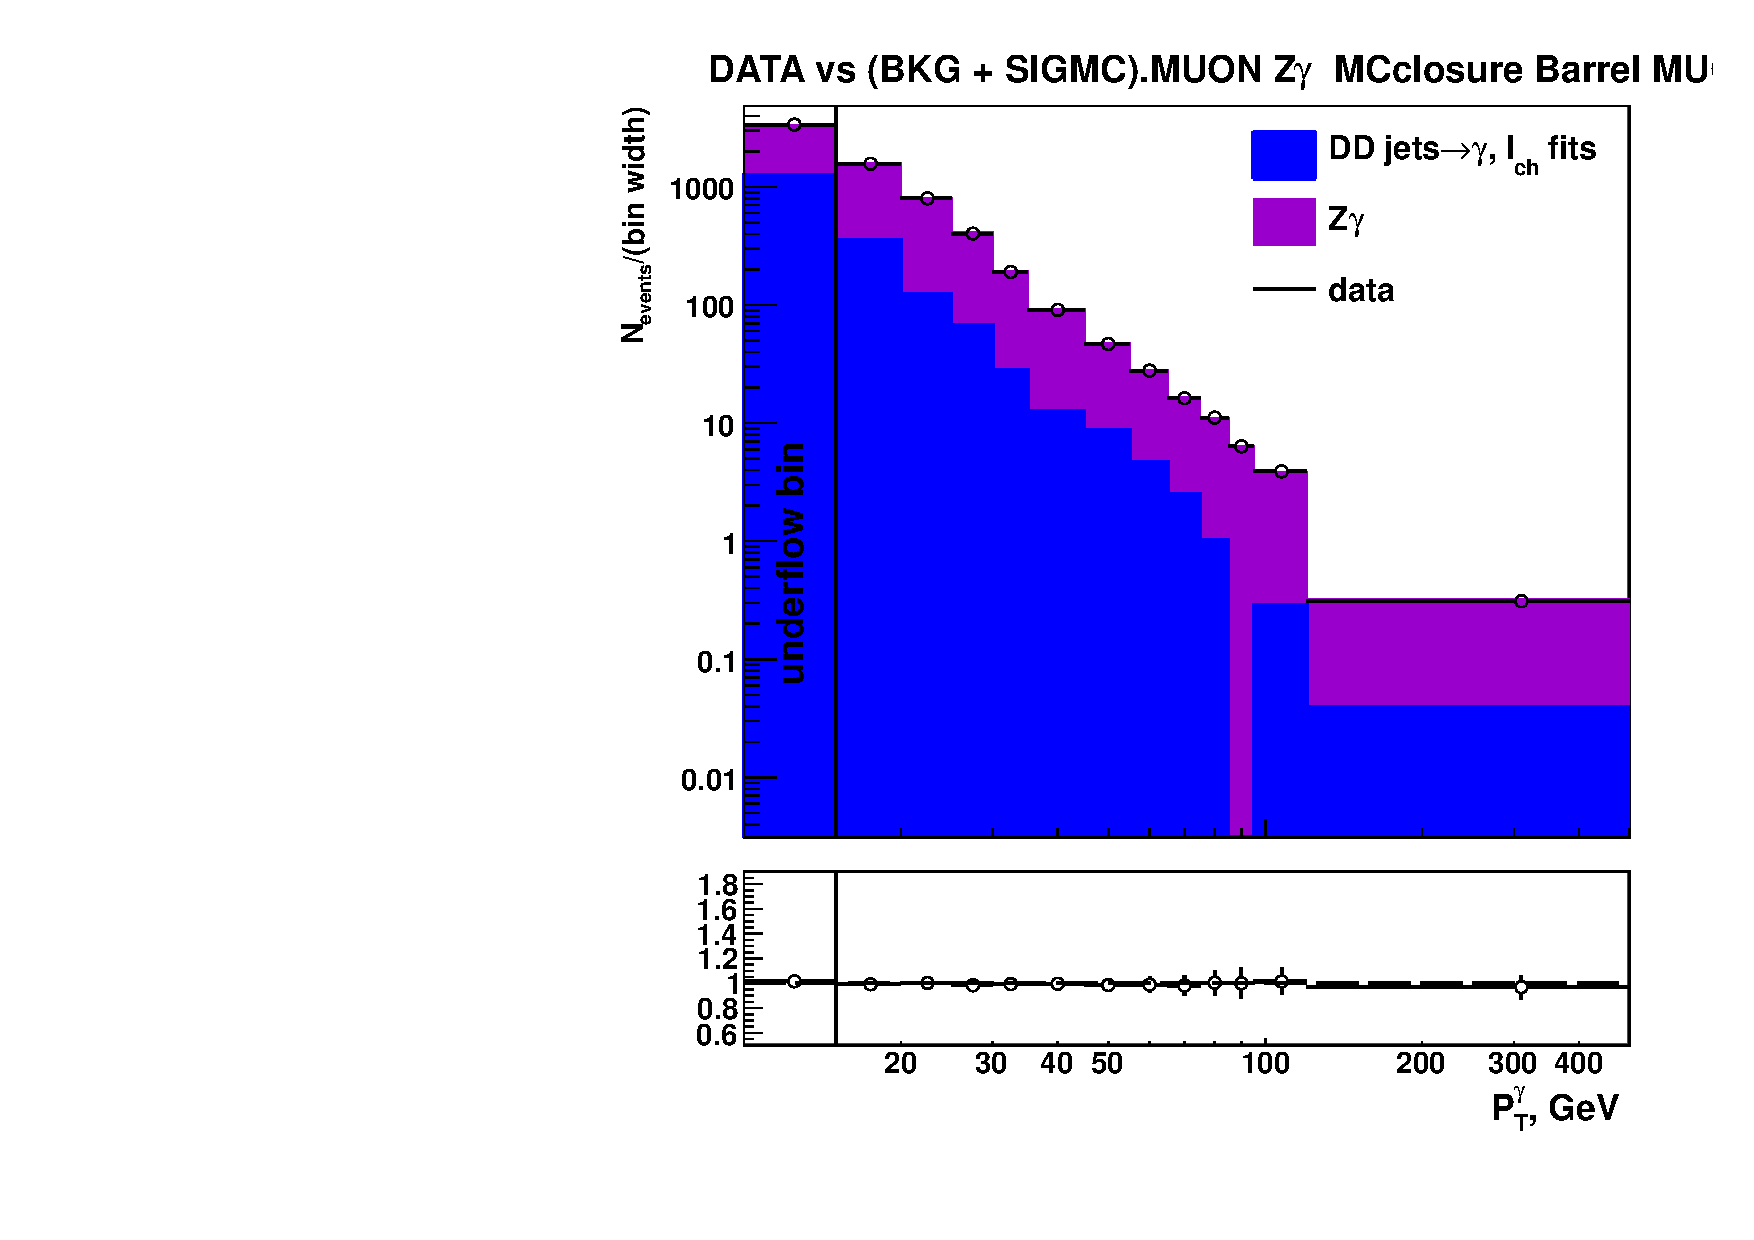
\includegraphics[width=0.45\textwidth]{../figs/figs_v11/MUON_ZGamma/PrepareYields/c_DATAvsBkgPlusSigMCc_MUON_ZGamma_TEMPL_CHISO_UNblind_MCclosure__Barrel__phoEt_MCclosure.pdf}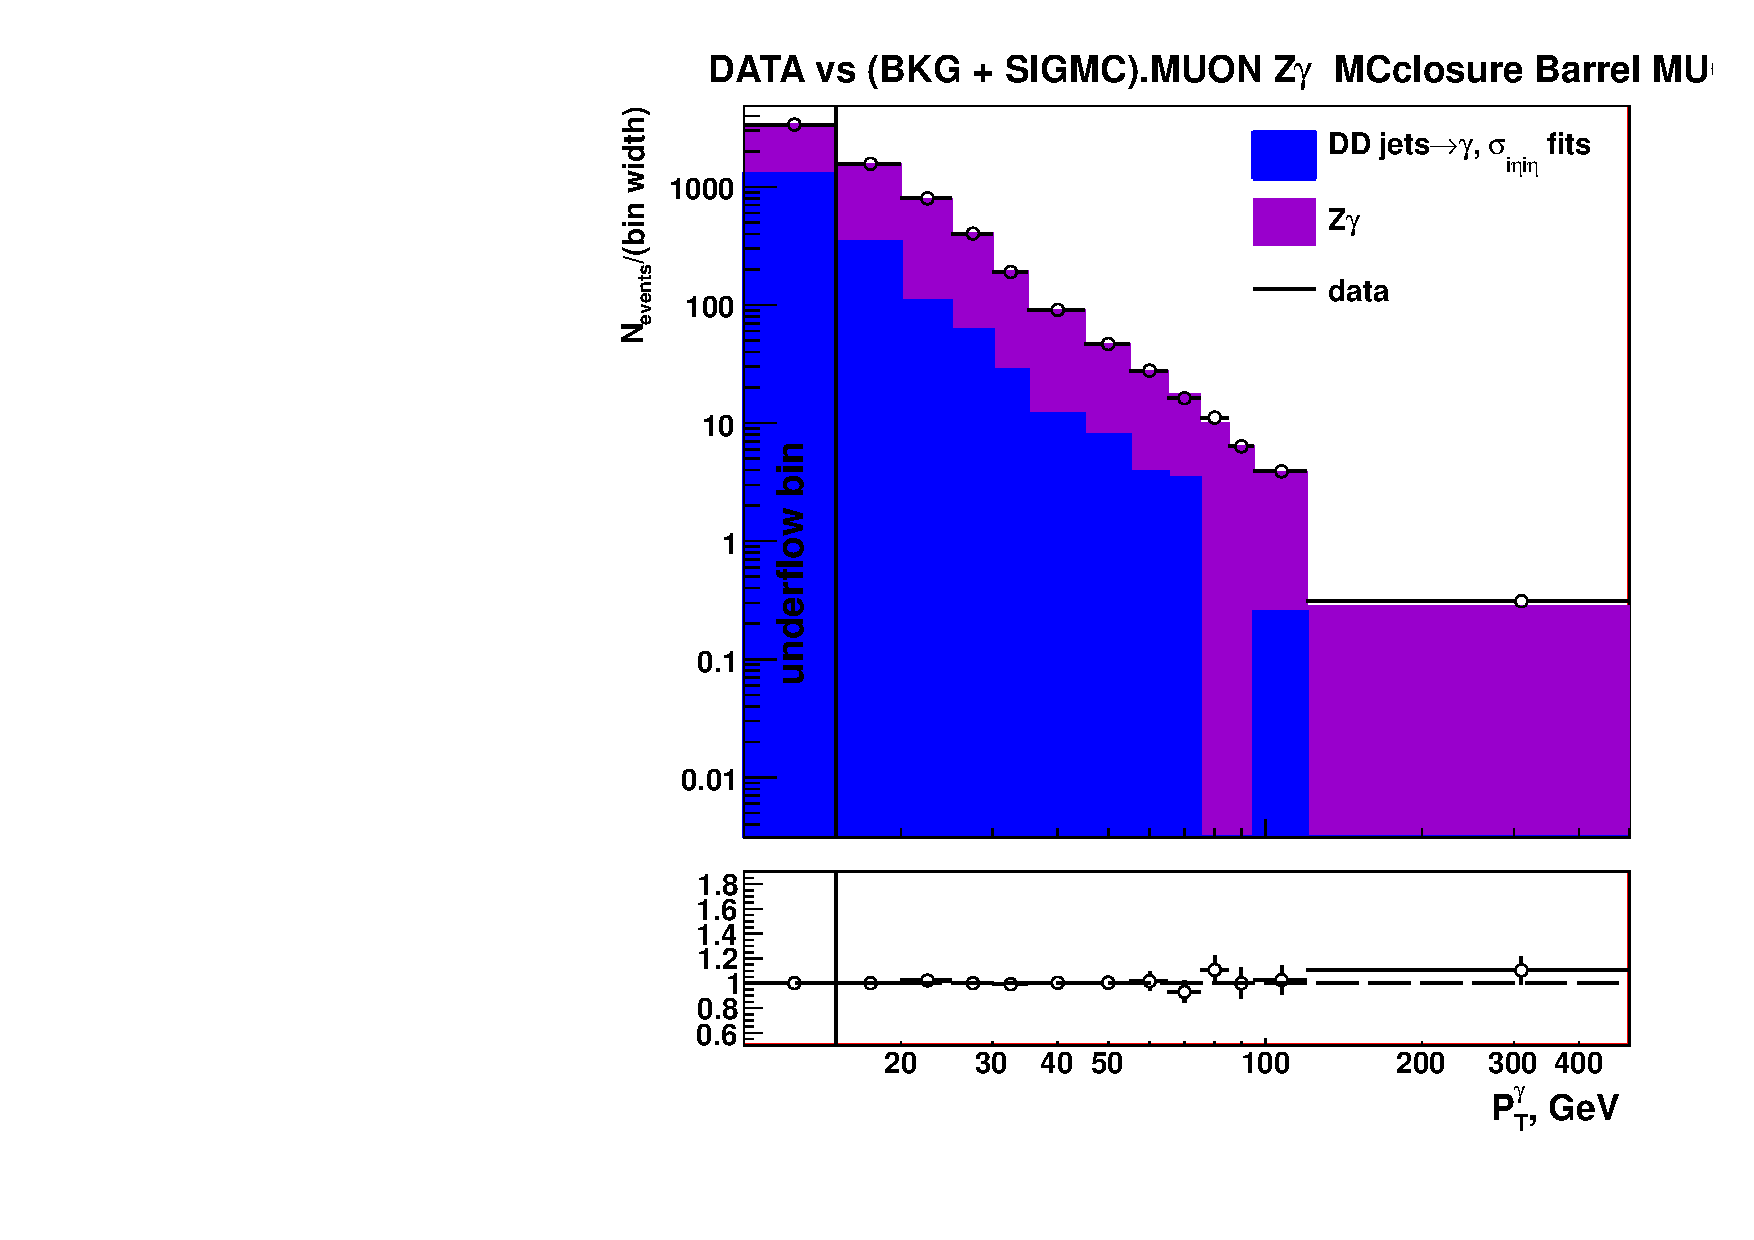
\includegraphics[width=0.45\textwidth]{../figs/figs_v11/MUON_ZGamma/PrepareYields/c_DATAvsBkgPlusSigMCc_MUON_ZGamma_TEMPL_SIHIH_UNblind_MCclosure__Barrel__phoEt_MCclosure.pdf}  \\
   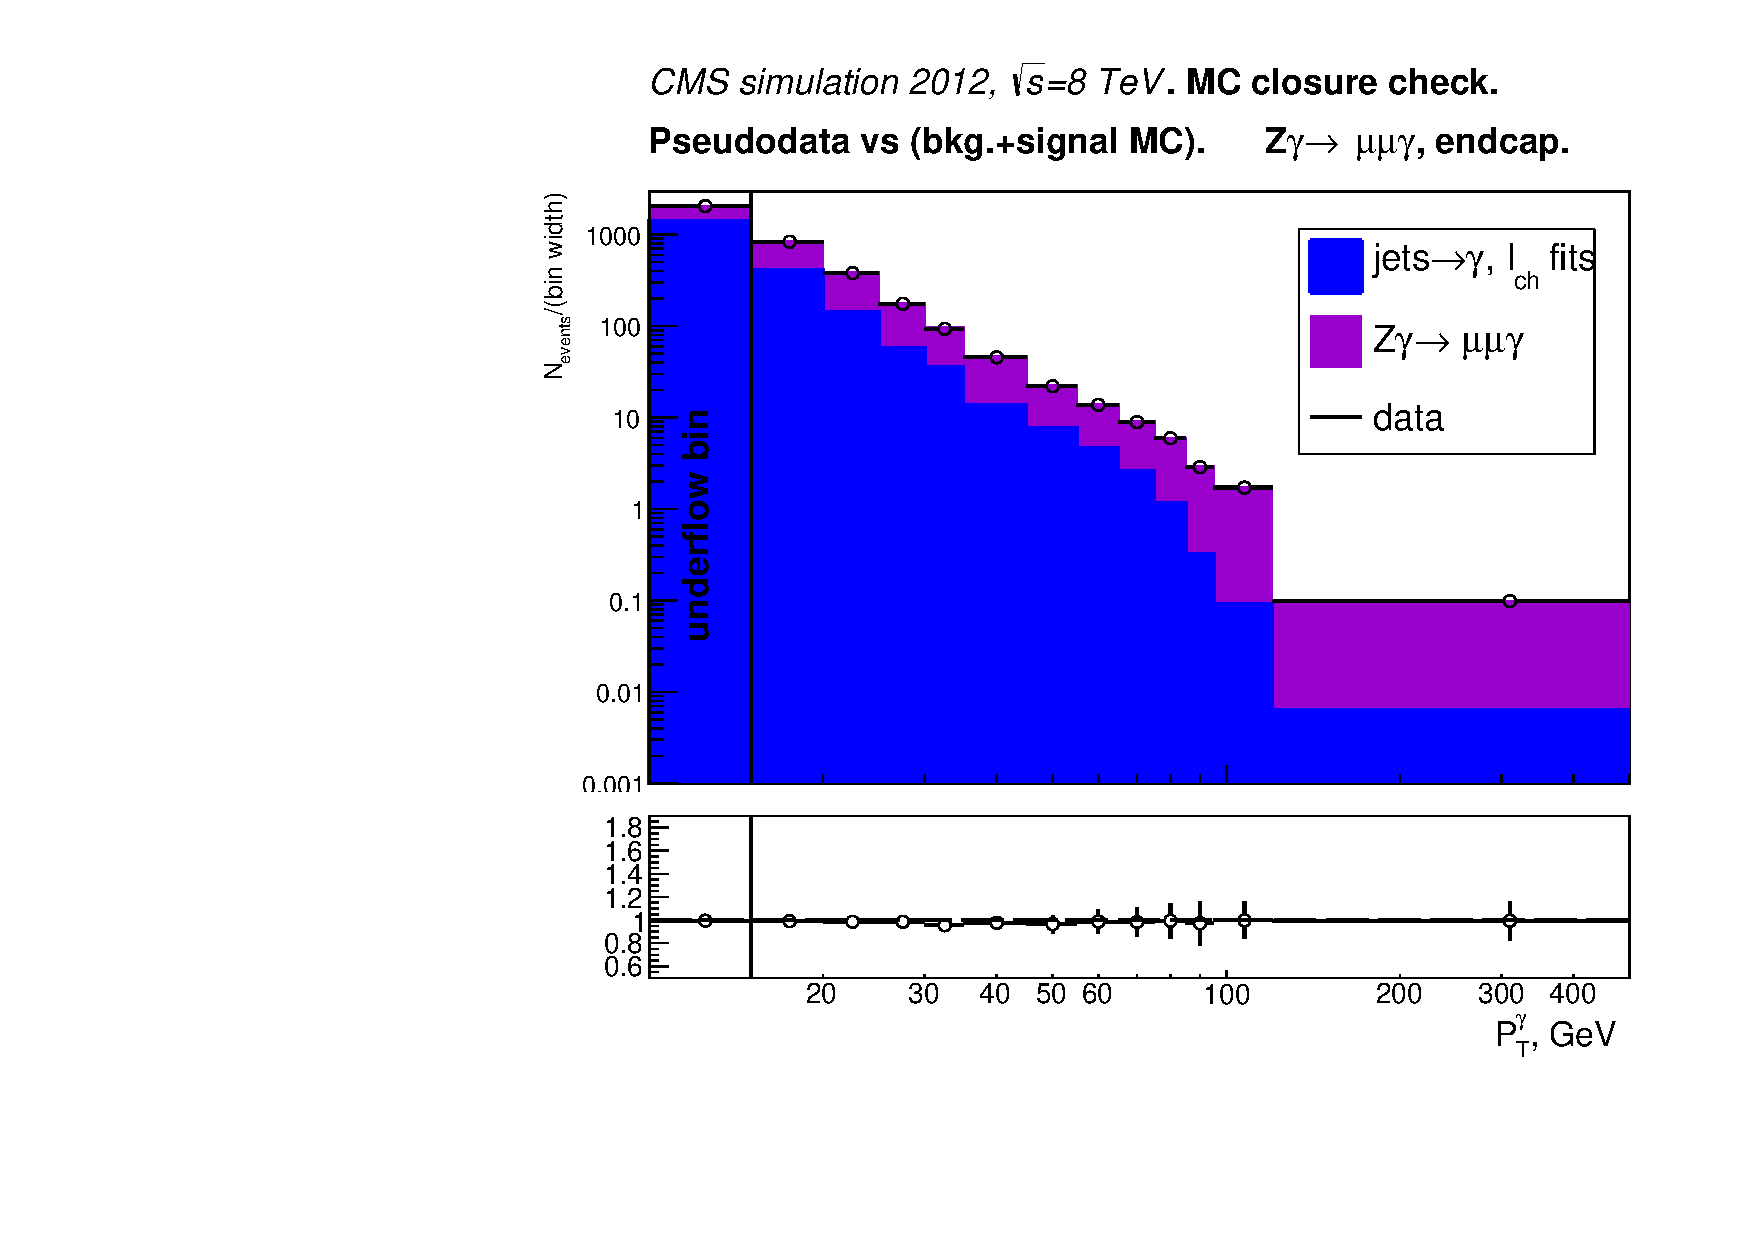
\includegraphics[width=0.45\textwidth]{../figs/figs_v11/MUON_ZGamma/PrepareYields/c_DATAvsBkgPlusSigMCc_MUON_ZGamma_TEMPL_CHISO_UNblind_MCclosure__Endcap__phoEt_MCclosure.pdf}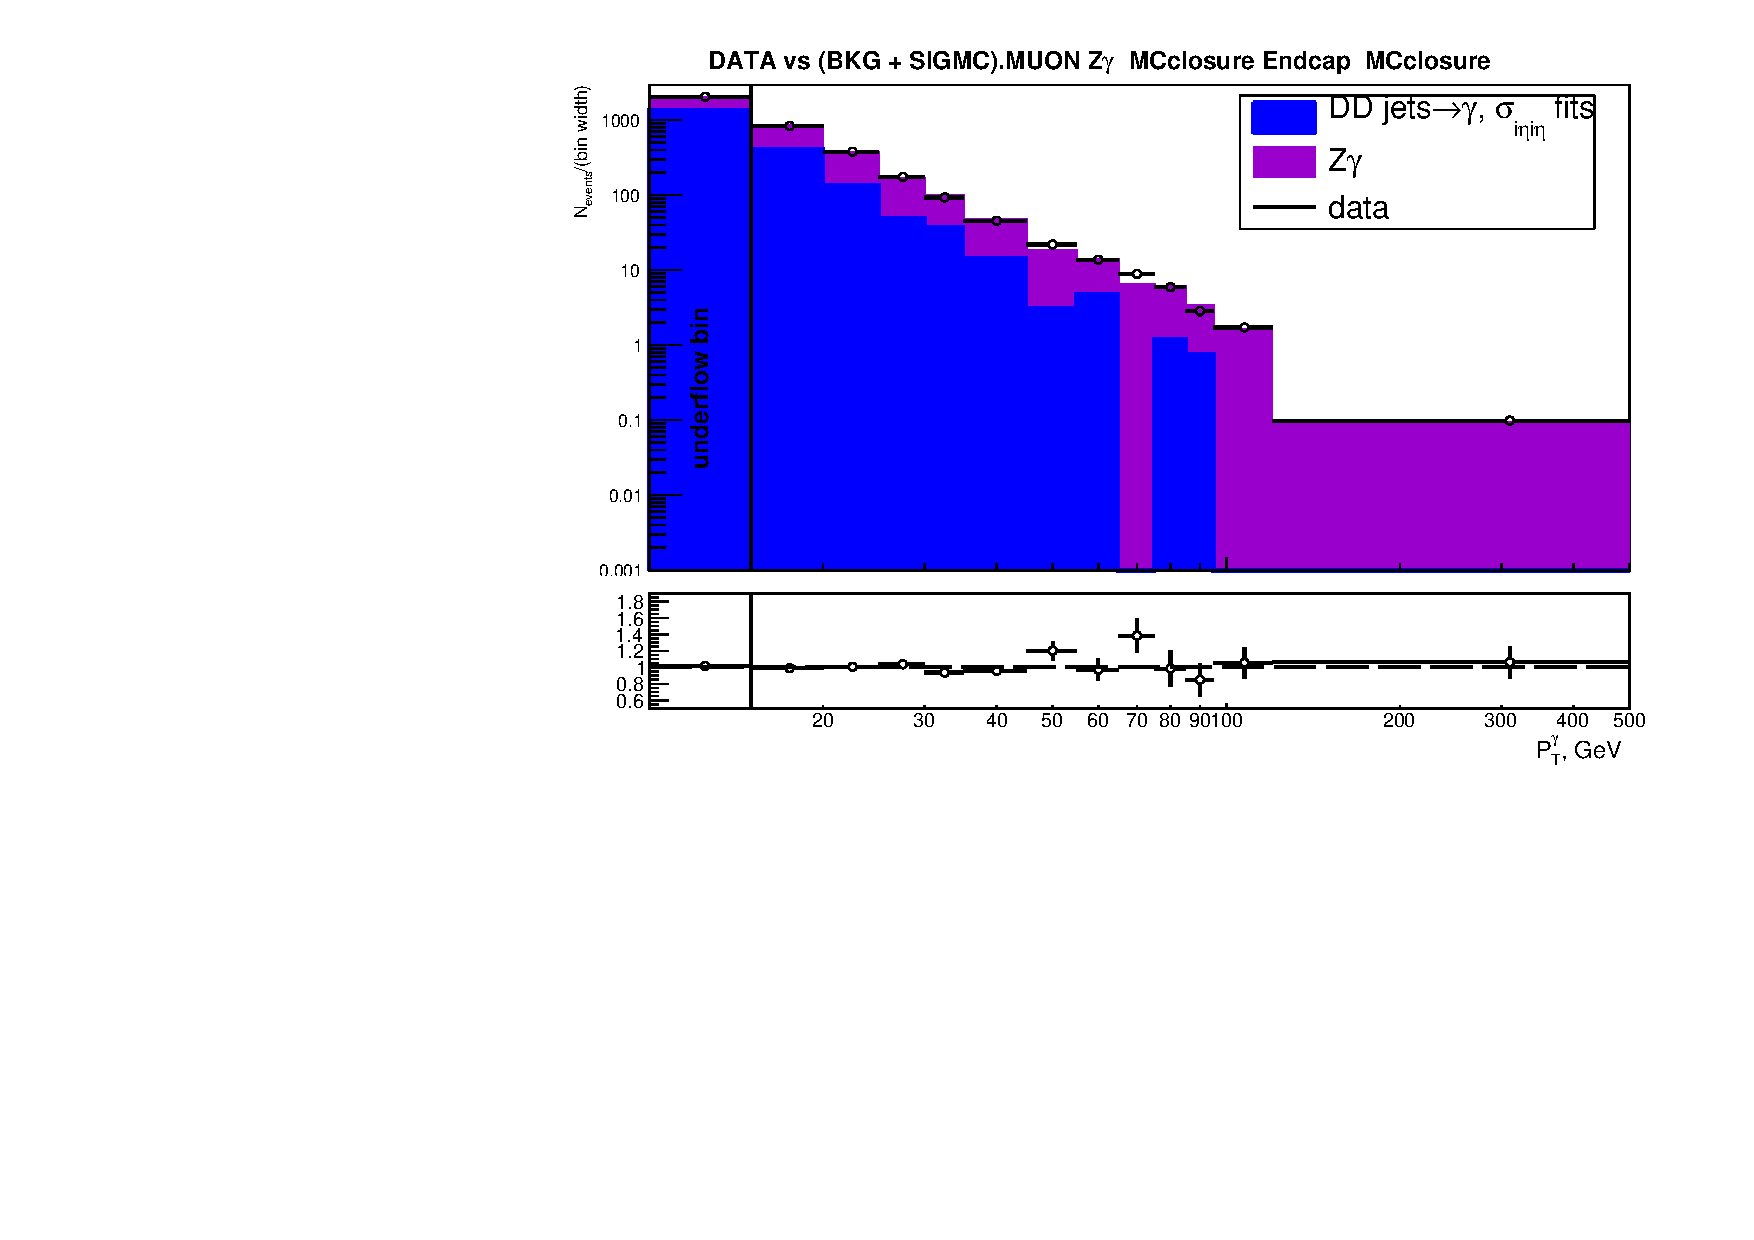
\includegraphics[width=0.45\textwidth]{../figs/figs_v11/MUON_ZGamma/PrepareYields/c_DATAvsBkgPlusSigMCc_MUON_ZGamma_TEMPL_SIHIH_UNblind_MCclosure__Endcap__phoEt_MCclosure.pdf}  \\
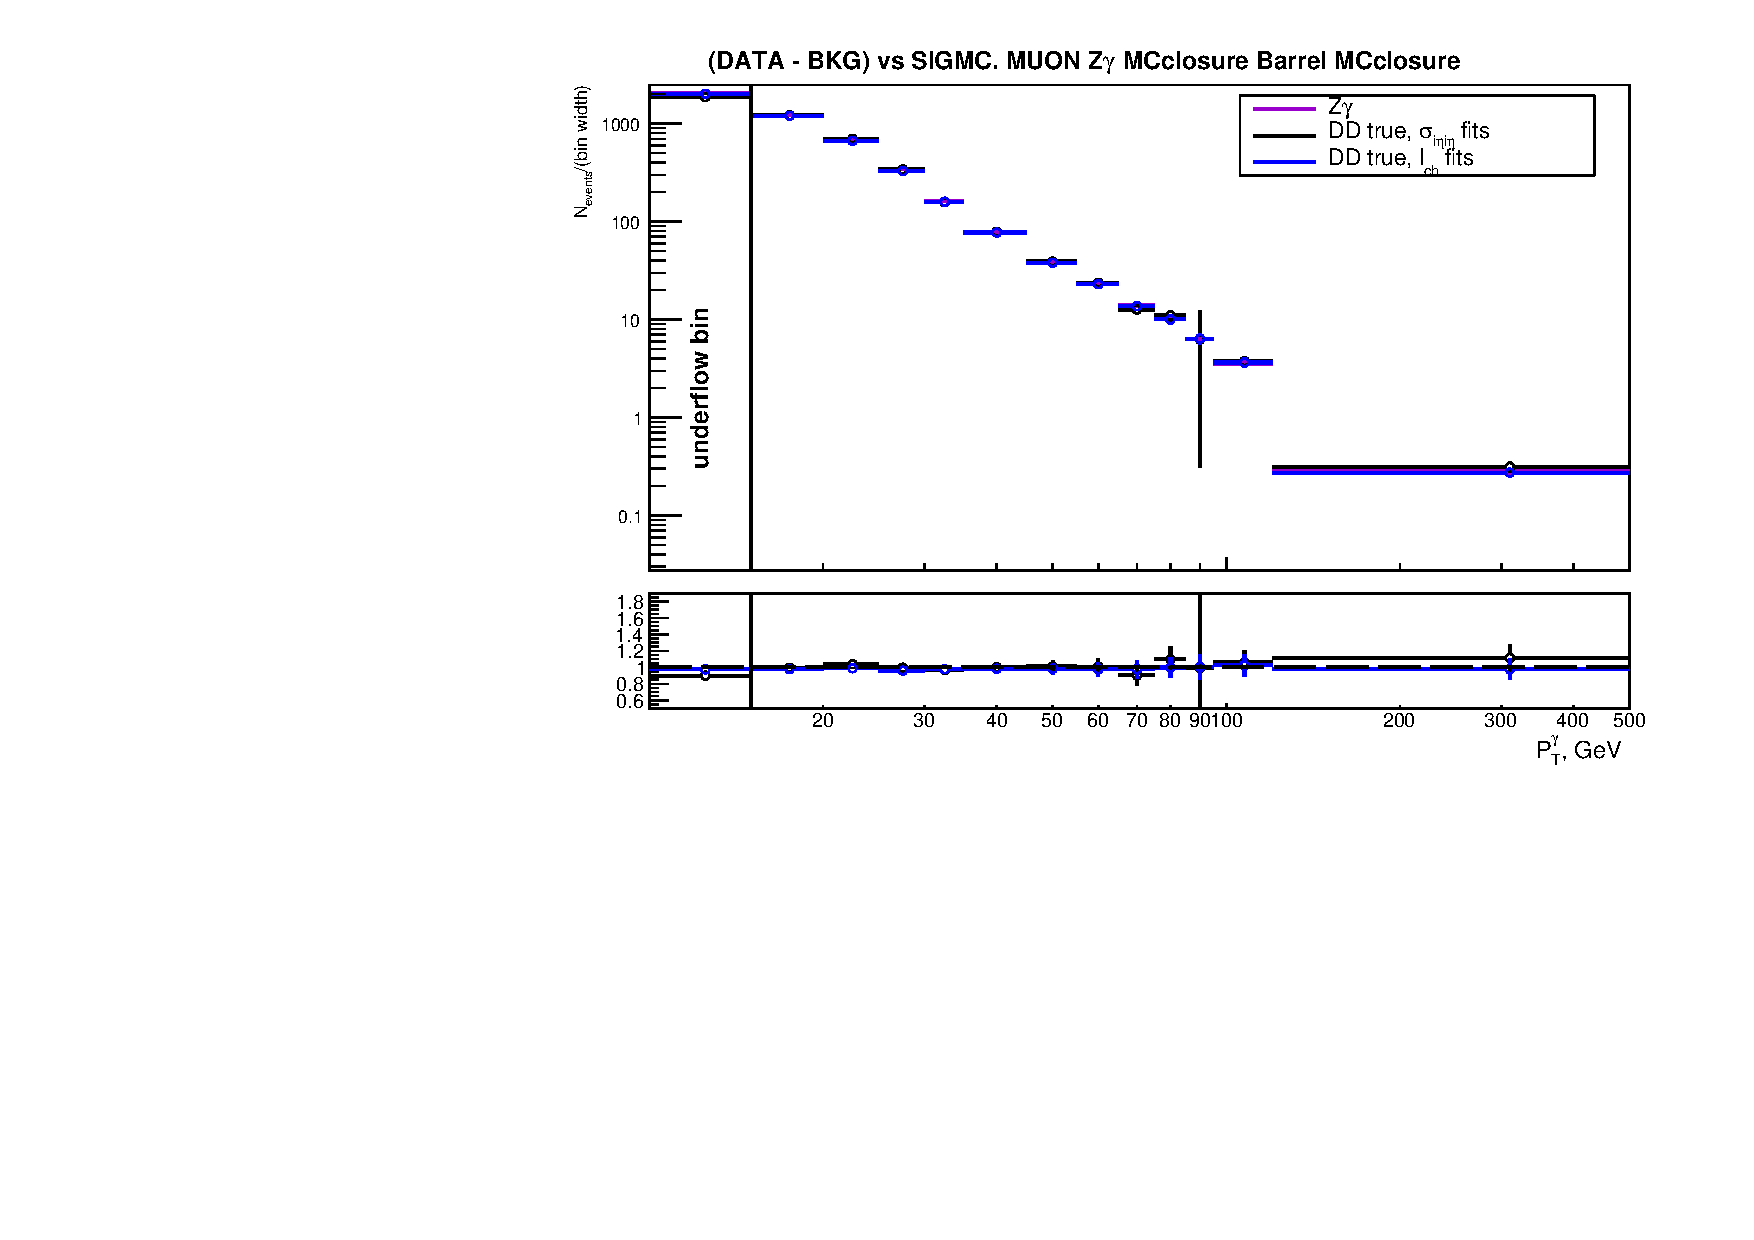
\includegraphics[width=0.45\textwidth]{../figs/figs_v11/MUON_ZGamma/PrepareYields/c_BkgSubtrDATAvsSIGMC_c_MUON_ZGamma__UNblind_MCclosure__Barrel__phoEt_MCclosure.pdf}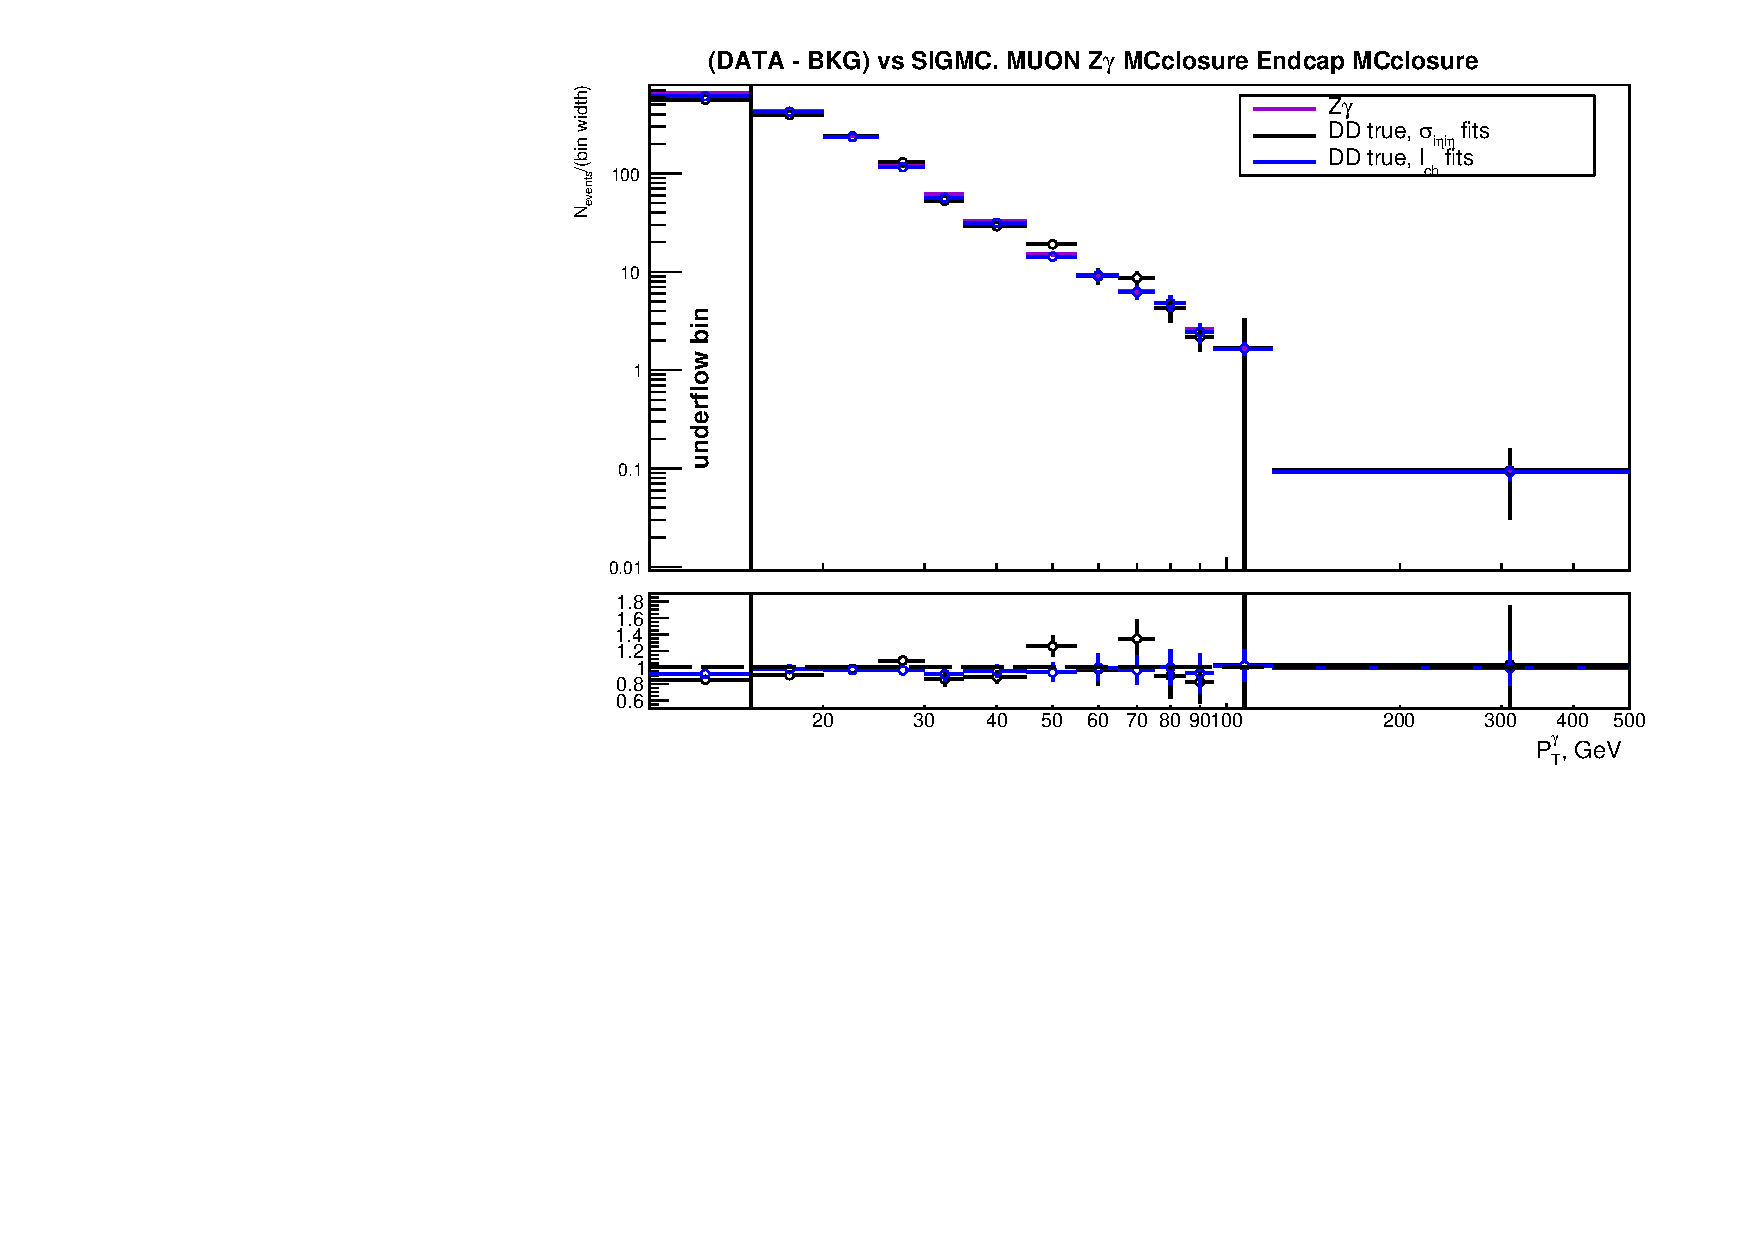
\includegraphics[width=0.45\textwidth]{../figs/figs_v11/MUON_ZGamma/PrepareYields/c_BkgSubtrDATAvsSIGMC_c_MUON_ZGamma__UNblind_MCclosure__Endcap__phoEt_MCclosure.pdf}\\
  \caption{$P_T^{\gamma}$ distribution of $Z\gamma$ candidates in the muon channel prepared with pseudodata. Top and middle: pseudodata vs fake-$\gamma$ background derived from the template method + real-$\gamma$ background predicted by dedicated MC samples + signal MC, with $I_{ch}$ (left) and $\sigma_{i\eta i\eta}$ (right) used as fit variables for candidates with photons in EB (top) and EE (middle). Bottom: data yields after full background subtraction vs signal MC for candidates with photons in in EB (left) and EE (right).}
  \label{fig:DDvsMC_Zg_MCclosure_MUON}
  \end{center}
\end{figure}

\begin{figure}[htb]
  \begin{center}
   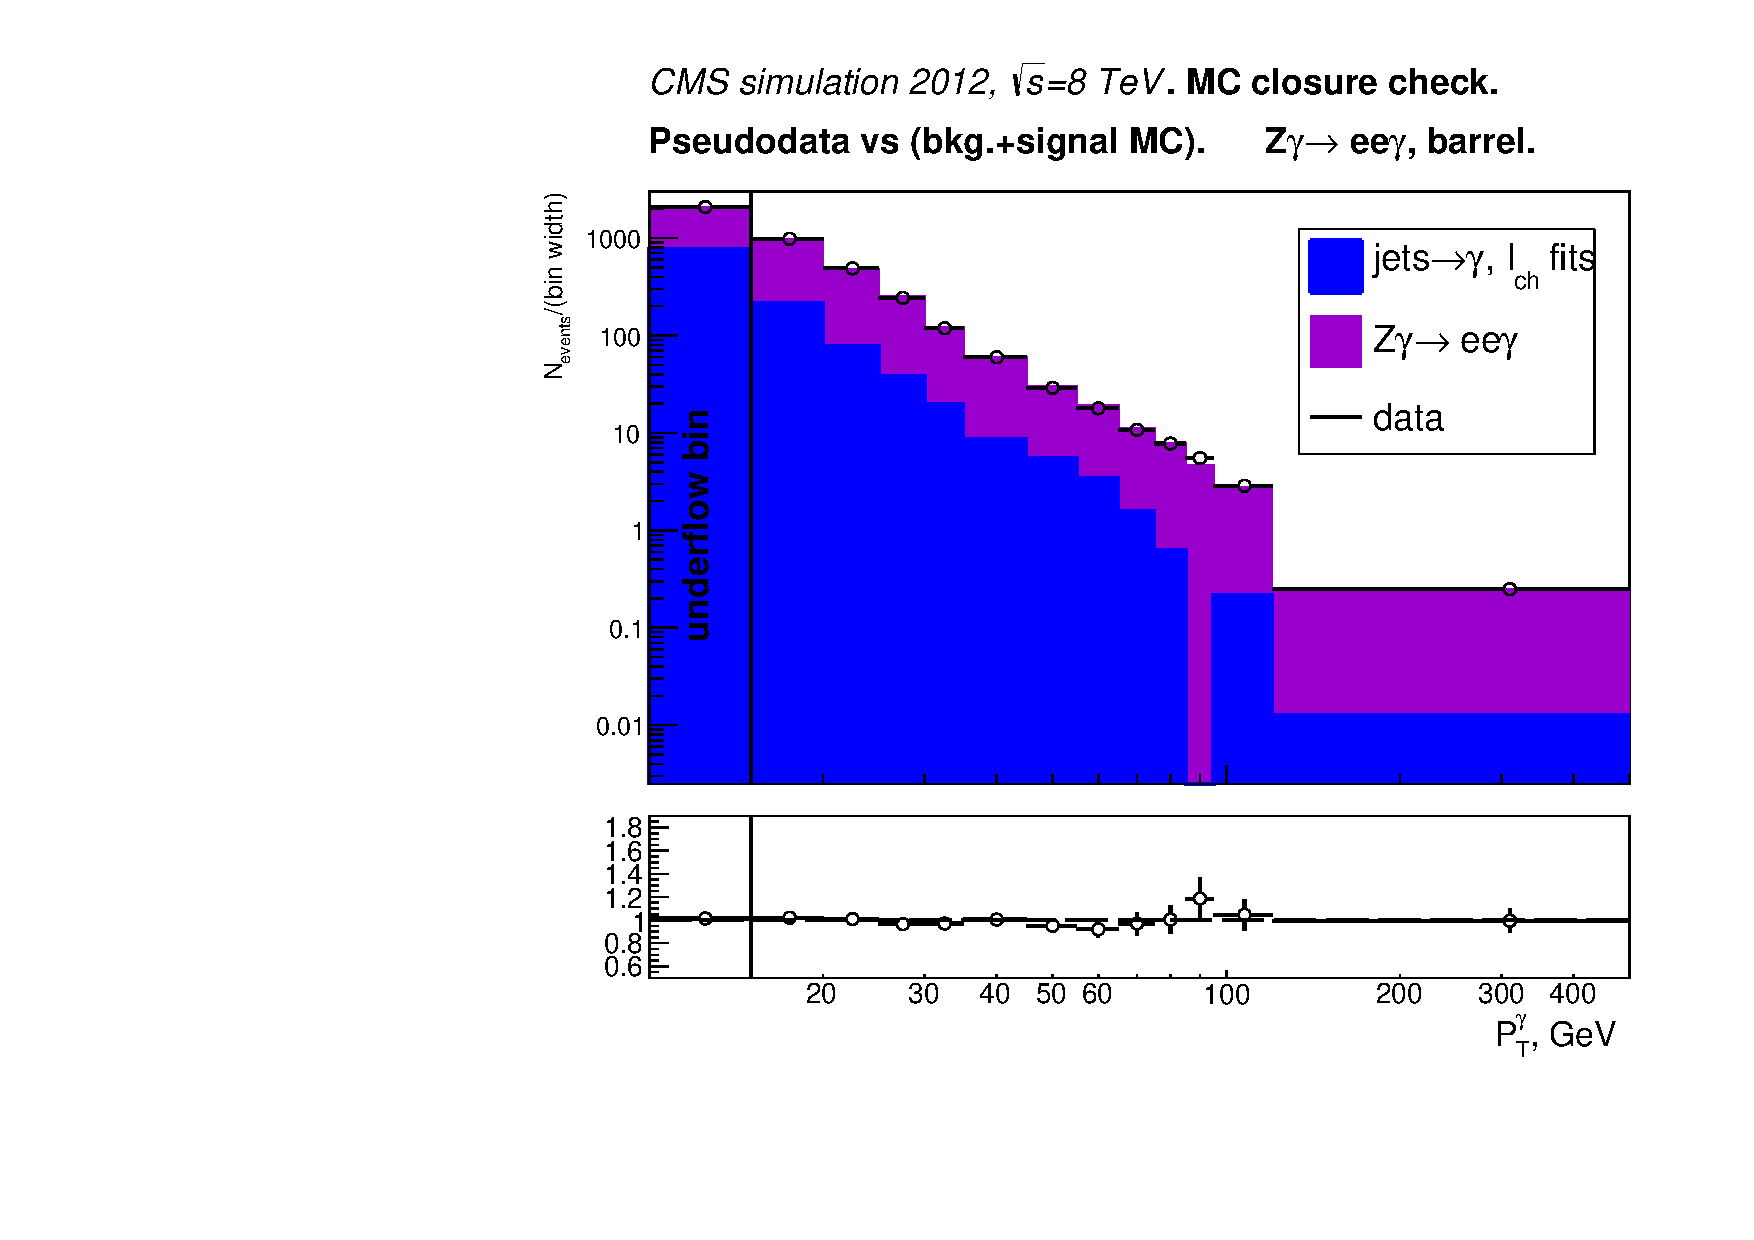
\includegraphics[width=0.45\textwidth]{../figs/figs_v11/ELECTRON_ZGamma/PrepareYields/c_DATAvsBkgPlusSigMCc_ELECTRON_ZGamma_TEMPL_CHISO_UNblind_MCclosure__Barrel__phoEt_MCclosure.pdf}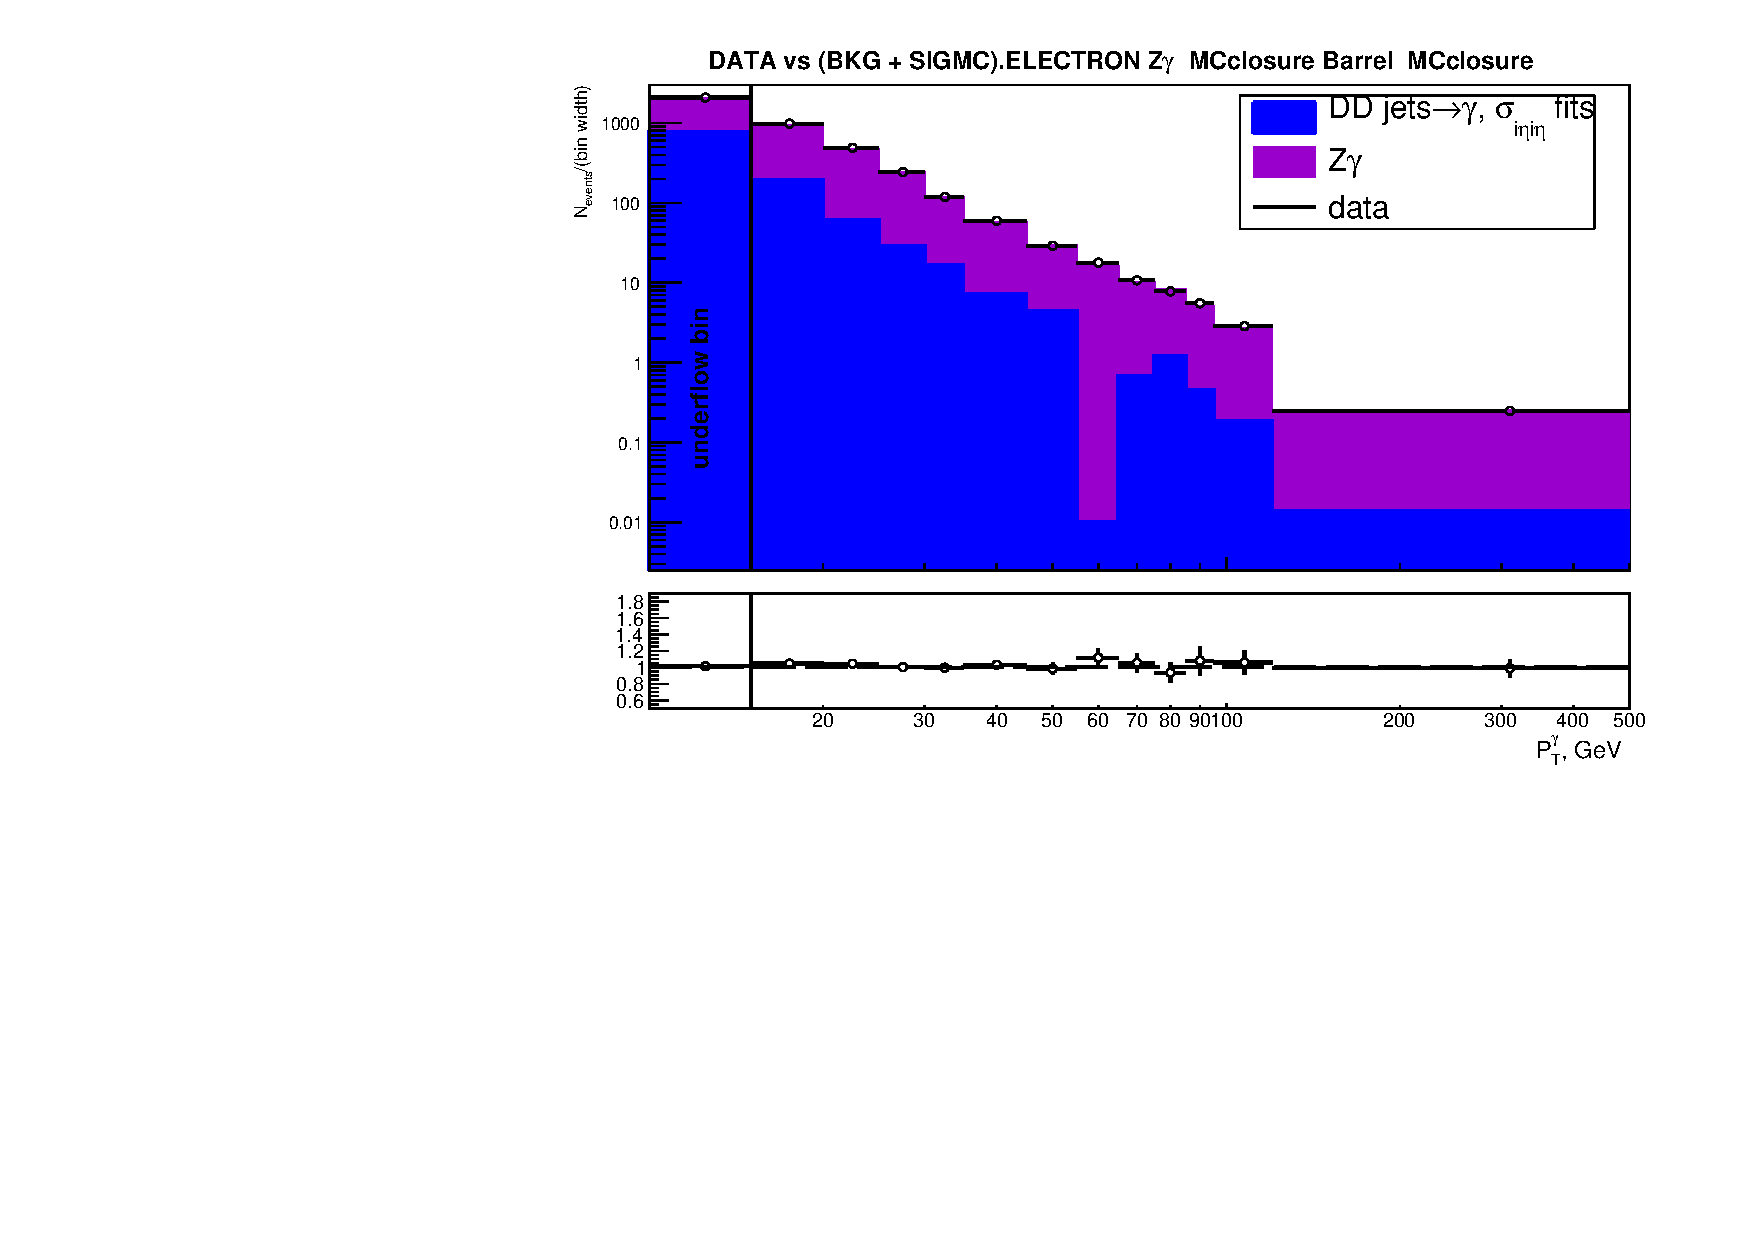
\includegraphics[width=0.45\textwidth]{../figs/figs_v11/ELECTRON_ZGamma/PrepareYields/c_DATAvsBkgPlusSigMCc_ELECTRON_ZGamma_TEMPL_SIHIH_UNblind_MCclosure__Barrel__phoEt_MCclosure.pdf}  \\
   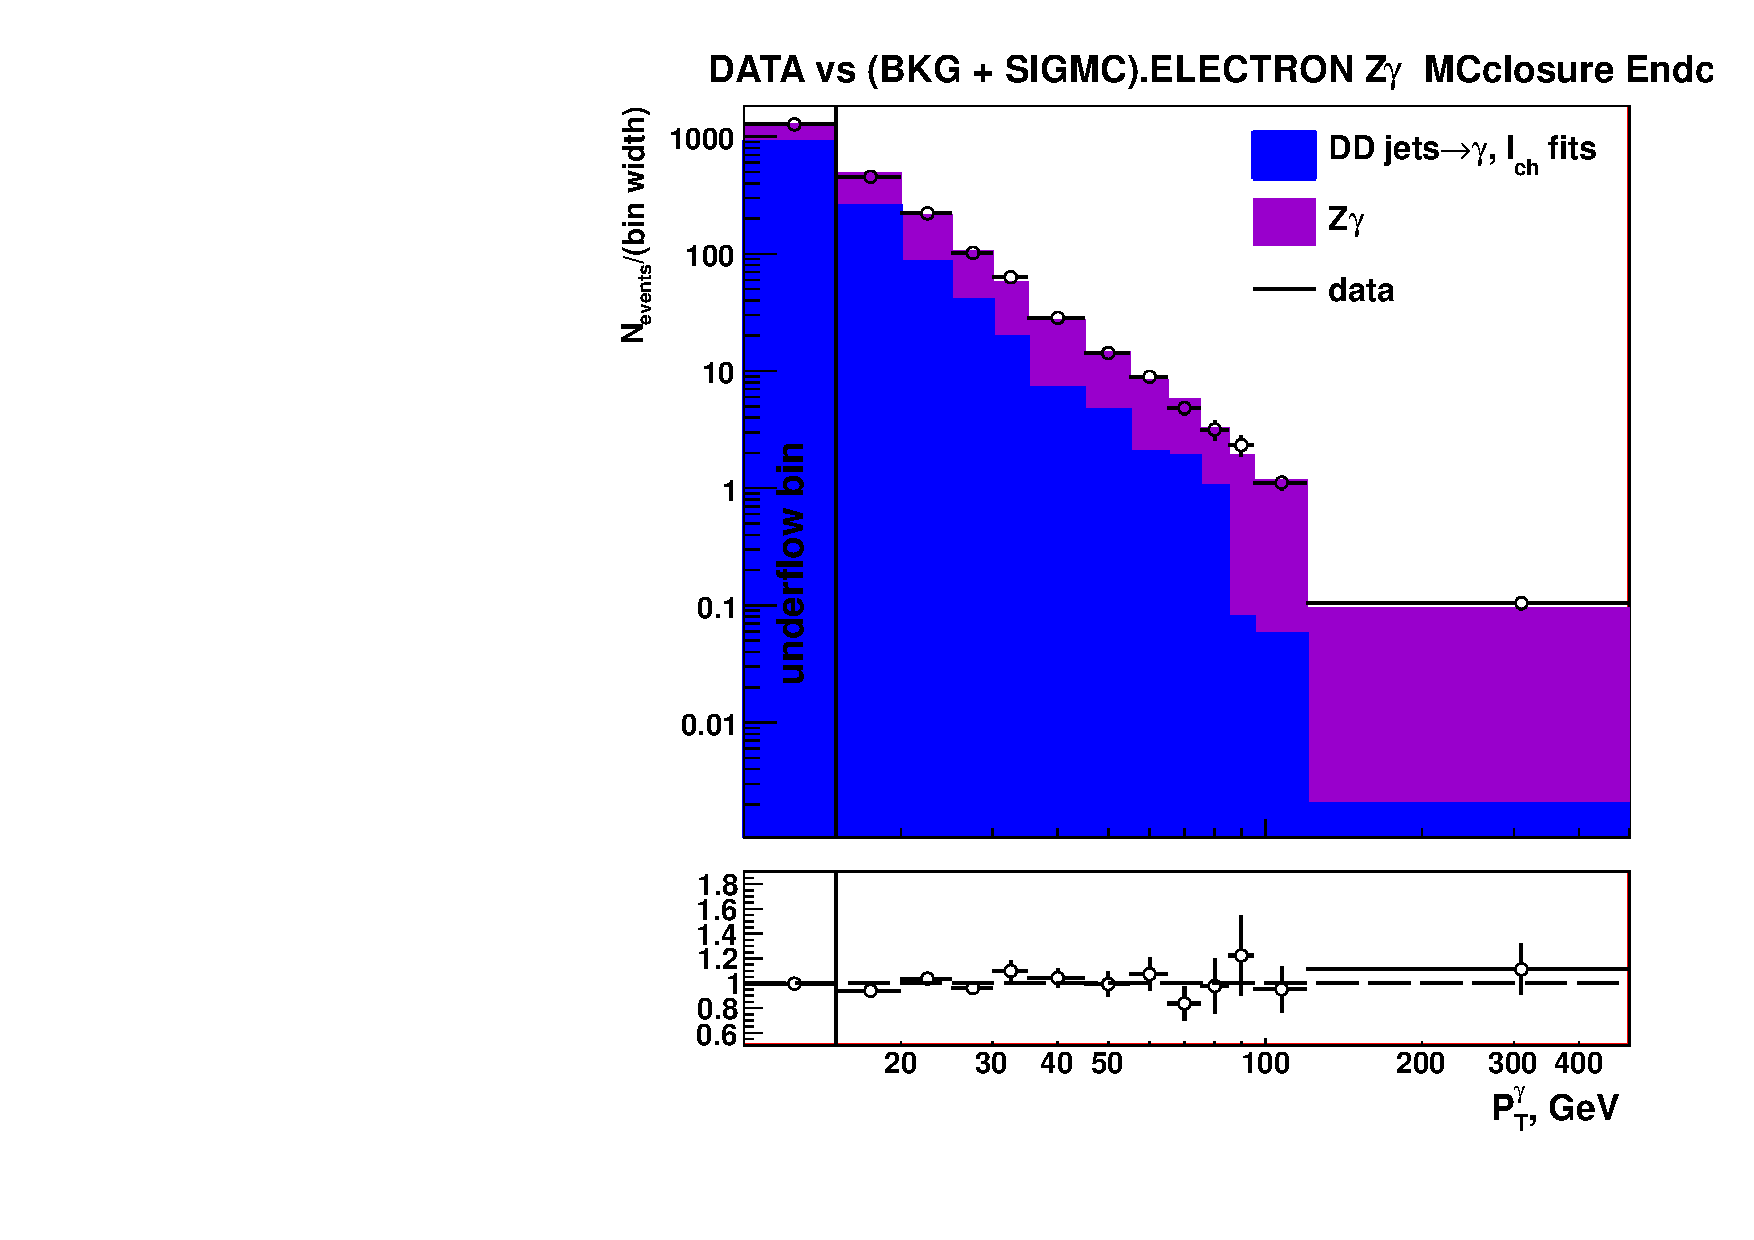
\includegraphics[width=0.45\textwidth]{../figs/figs_v11/ELECTRON_ZGamma/PrepareYields/c_DATAvsBkgPlusSigMCc_ELECTRON_ZGamma_TEMPL_CHISO_UNblind_MCclosure__Endcap__phoEt_MCclosure.pdf}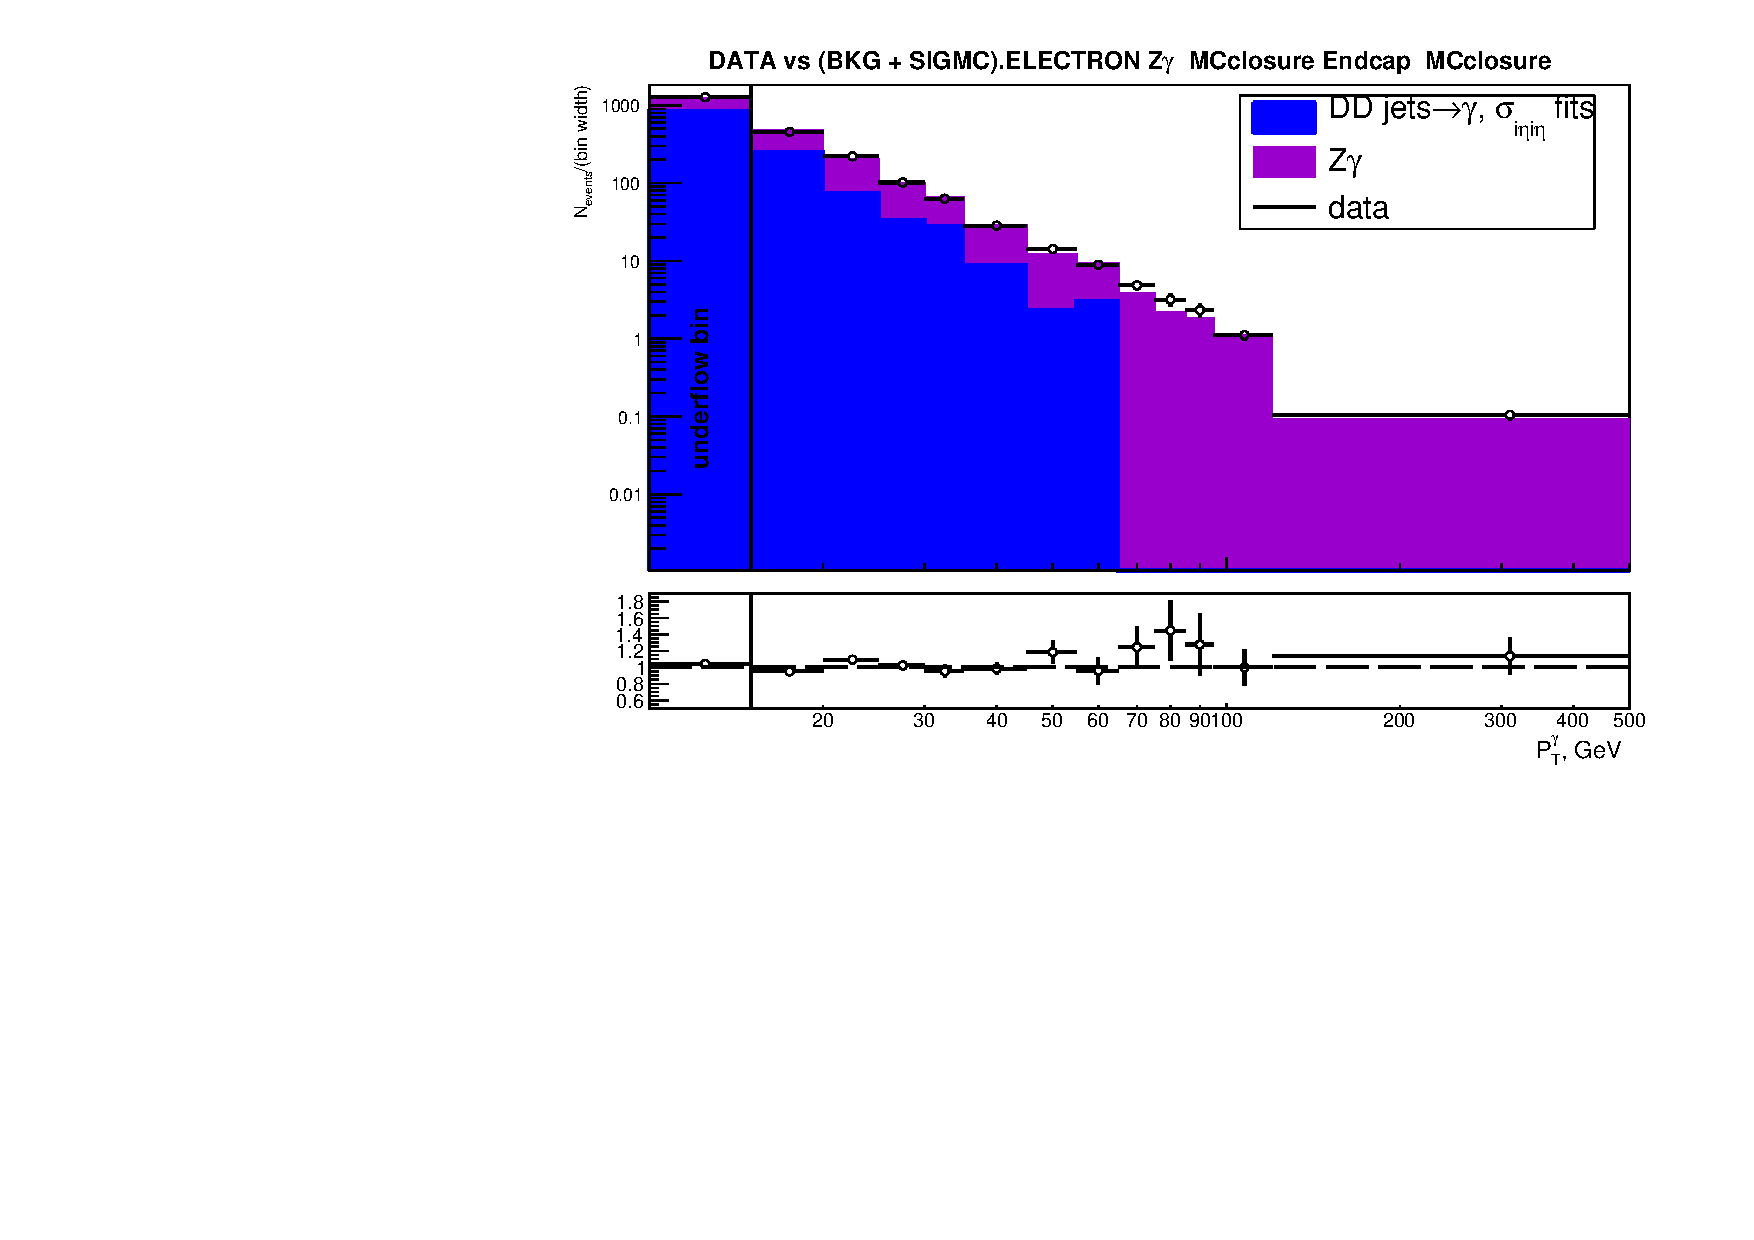
\includegraphics[width=0.45\textwidth]{../figs/figs_v11/ELECTRON_ZGamma/PrepareYields/c_DATAvsBkgPlusSigMCc_ELECTRON_ZGamma_TEMPL_SIHIH_UNblind_MCclosure__Endcap__phoEt_MCclosure.pdf}  \\
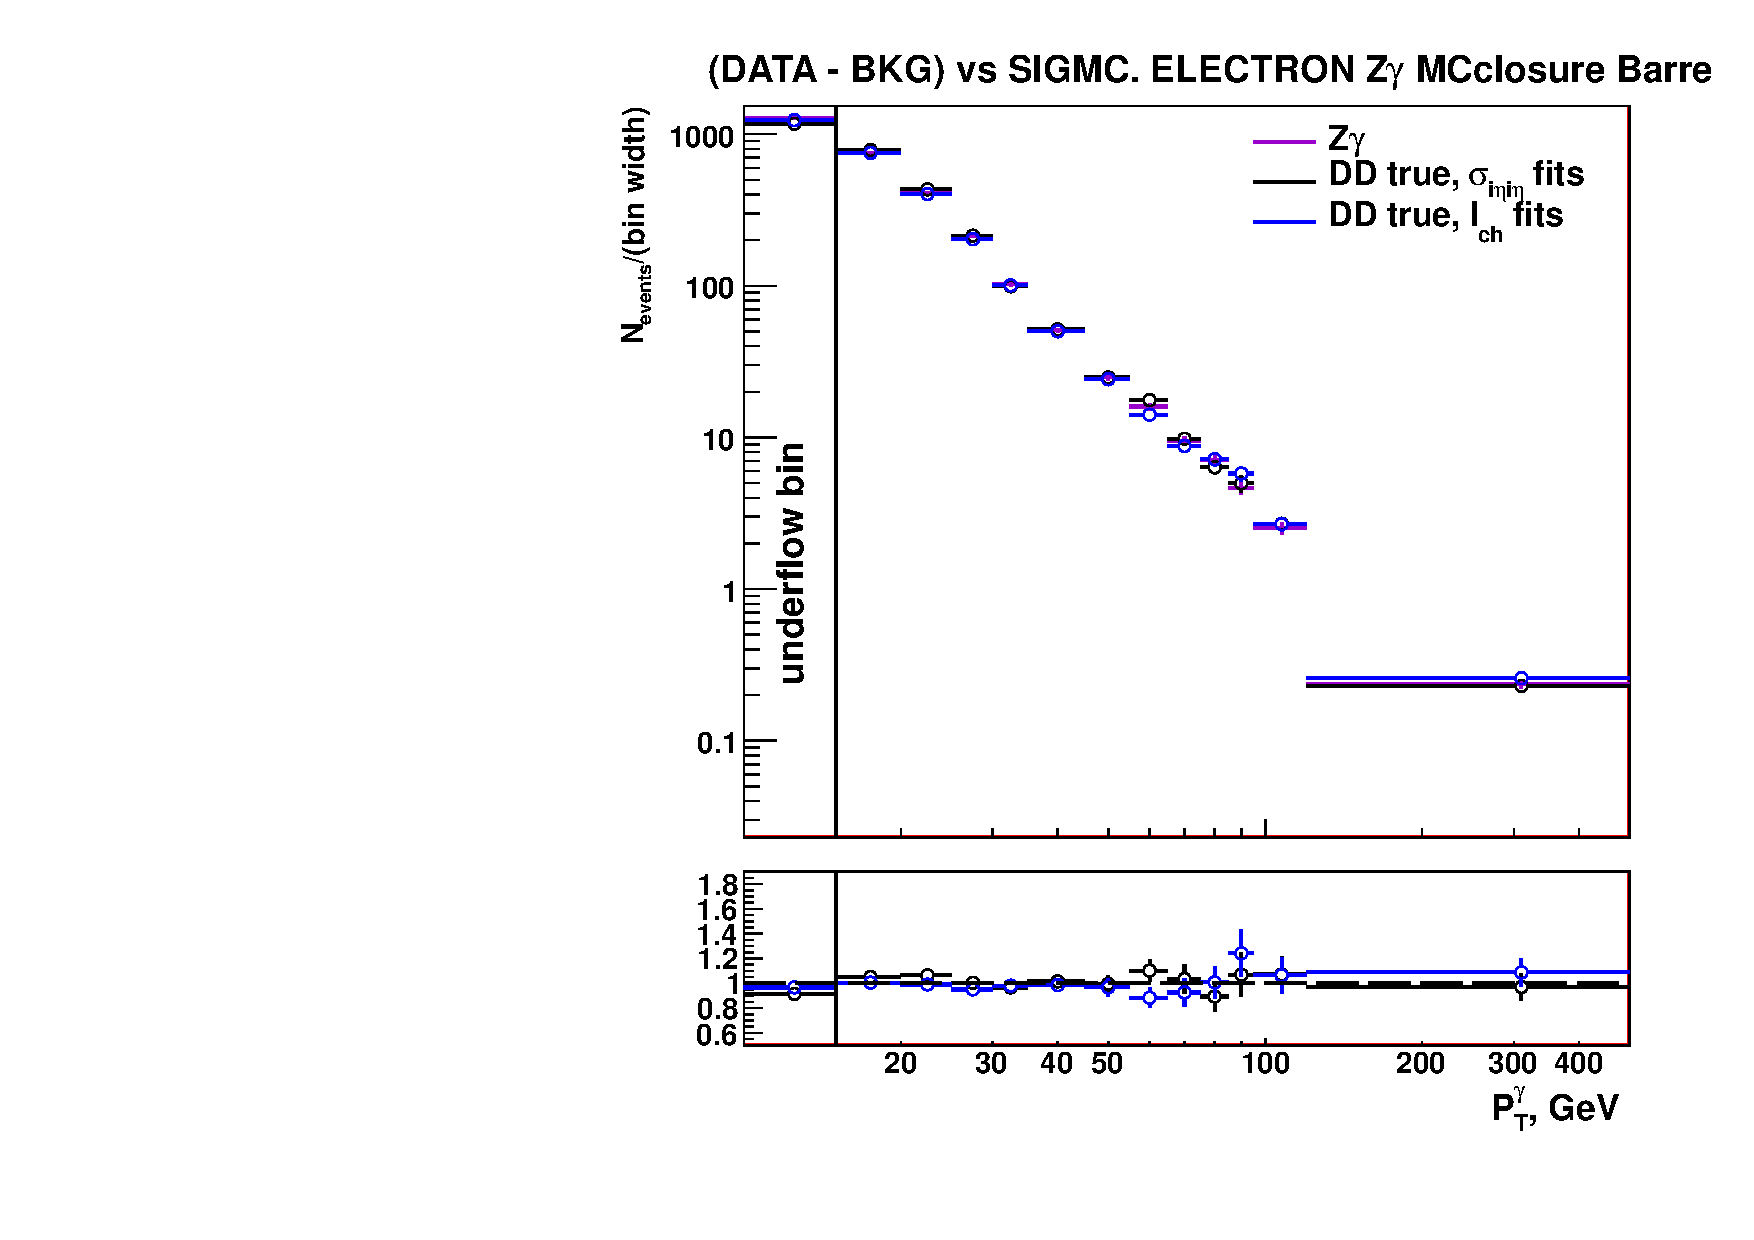
\includegraphics[width=0.45\textwidth]{../figs/figs_v11/ELECTRON_ZGamma/PrepareYields/c_BkgSubtrDATAvsSIGMC_c_ELECTRON_ZGamma__UNblind_MCclosure__Barrel__phoEt_MCclosure.pdf}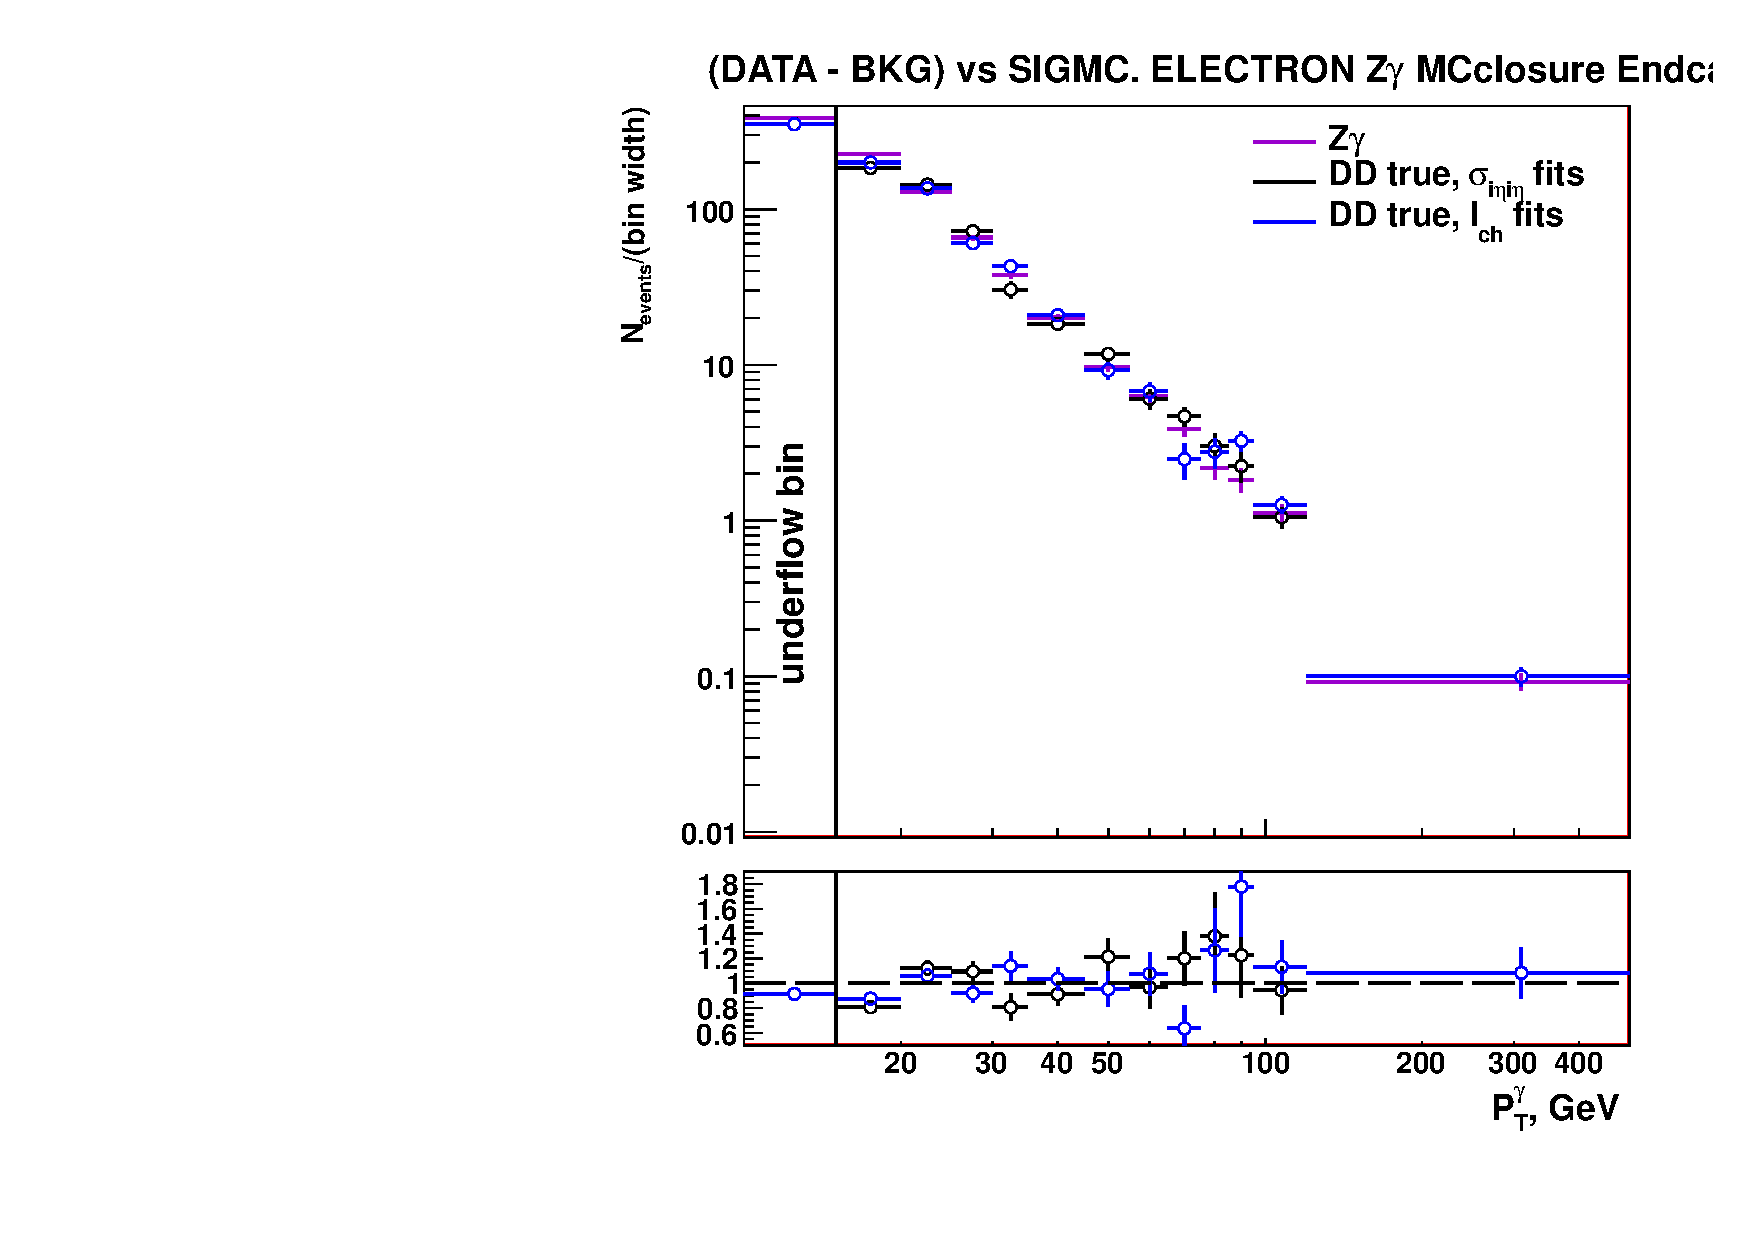
\includegraphics[width=0.45\textwidth]{../figs/figs_v11/ELECTRON_ZGamma/PrepareYields/c_BkgSubtrDATAvsSIGMC_c_ELECTRON_ZGamma__UNblind_MCclosure__Endcap__phoEt_MCclosure.pdf}\\
  \caption{$P_T^{\gamma}$ distribution of $Z\gamma$ candidates in the electron channel prepared with pseudodata. Top and middle: pseudodata vs fake-$\gamma$ background derived from the template method + real-$\gamma$ background predicted by dedicated MC samples + signal MC, with $I_{ch}$ (left) and $\sigma_{i\eta i\eta}$ (right) used as fit variables for candidates with photons in EB (top) and EE (middle). Bottom: data yields after full background subtraction vs signal MC for candidates with photons in in EB (left) and EE (right).}
  \label{fig:DDvsMC_Zg_MCclosure_ELECTRON}
  \end{center}
\end{figure}

\clearpage

\begin{table}[h]
  \scriptsize
  \begin{center}
  \caption{Relative uncertainties [\%] on the $Z\gamma$ differential and total (row ``total'') cross section in the muon channel.}
  \begin{tabular}{|c|c|c|c|c|c|c|c|c|}
    $P_T^{\gamma}$,  & err & syst & $Z\gamma$ MC & $A \times \epsilon$ & syst & unf & syst & syst + stat\\
    GeV  & stat & $|N_{Ich}-N_{\sigma{i\eta i\eta}}|$ & norm & MC stat & lumi & MC stat & total & total\\ \hline
    total  & 1 & 1 & 1 & 0 & 3 & 1 & 3 & 3 \\ \hline
%    10-15 & 2 & 3 & 3 & 1 & 3 & 2 & 5 & 5 \\ \hline
    15-20 & 2 & 2 & 2 & 1 & 3 & 2 & 4 & 5 \\ \hline
    20-25 & 2 & 2 & 3 & 1 & 3 & 2 & 5 & 5 \\ \hline
    25-30 & 3 & 3 & 4 & 2 & 3 & 3 & 7 & 8 \\ \hline
    30-35 & 4 & 6 & 5 & 3 & 3 & 5 & 10 & 10 \\ \hline
    35-45 & 4 & 3 & 6 & 3 & 3 & 4 & 9 & 9 \\ \hline
    45-55 & 6 & 8 & 8 & 4 & 3 & 6 & 14 & 15 \\ \hline
    55-65 & 7 & 5 & 7 & 5 & 3 & 7 & 13 & 14 \\ \hline
    65-75 & 9 & 7 & 8 & 6 & 3 & 9 & 16 & 18 \\ \hline
    75-85 & 10 & 8 & 6 & 7 & 3 & 10 & 16 & 19 \\ \hline
    85-95 & 12 & 8 & 8 & 9 & 3 & 12 & 19 & 23 \\ \hline
    95-120 & 11 & 10 & 6 & 8 & 3 & 11 & 18 & 21 \\ \hline
    120-500 & 8 & 5 & 9 & 7 & 3 & 9 & 16 & 18 \\ \hline
  \end{tabular}
  \label{tab:systInPercent_MUON_ZGamma}
  \end{center}
\end{table}

\begin{table}[h]
  \scriptsize
  \begin{center}
  \caption{Relative uncertainties [\%] on the $Z\gamma$ differential and total (row ``total'') cross section in the electron channel.}
  \begin{tabular}{|c|c|c|c|c|c|c|c|c|}
    $P_T^{\gamma}$,  & err & syst & $Z\gamma$ MC & $A\times \epsilon$ & syst & unf & syst & syst + stat\\
    GeV  & stat & $|N_{Ich}-N_{\sigma{i\eta i\eta}}|$ & norm & MC stat & lumi & MC stat & total & total\\ \hline
    total  & 1 & 1 & 1 & 0 & 3 & 1 & 3 & 4 \\ \hline
%    10-15 & 2 & 2 & 3 & 1 & 3 & 2 & 5 & 5 \\ \hline
    15-20 & 2 & 3 & 3 & 1 & 3 & 2 & 5 & 6 \\ \hline
    20-25 & 3 & 2 & 3 & 1 & 3 & 3 & 5 & 6 \\ \hline
    25-30 & 4 & 3 & 4 & 2 & 3 & 4 & 7 & 8 \\ \hline
    30-35 & 5 & 4 & 5 & 3 & 3 & 6 & 10 & 11 \\ \hline
    35-45 & 5 & 4 & 6 & 3 & 3 & 5 & 10 & 11 \\ \hline
    45-55 & 6 & 6 & 6 & 4 & 3 & 7 & 11 & 13 \\ \hline
    55-65 & 9 & 7 & 8 & 5 & 3 & 9 & 15 & 17 \\ \hline
    65-75 & 10 & 8 & 8 & 7 & 3 & 11 & 18 & 20 \\ \hline
    75-85 & 14 & 11 & 12 & 9 & 3 & 16 & 25 & 28 \\ \hline
    85-95 & 15 & 9 & 6 & 10 & 3 & 17 & 23 & 28 \\ \hline
    95-120 & 10 & 5 & 6 & 9 & 3 & 11 & 16 & 19 \\ \hline
    120-500 & 9 & 3 & 7 & 8 & 3 & 10 & 15 & 17 \\ \hline
  \end{tabular}
  \label{tab:systInPercent_ELECTRON_ZGamma}
  \end{center}
\end{table}

\begin{figure}[htb]
  \begin{center}
   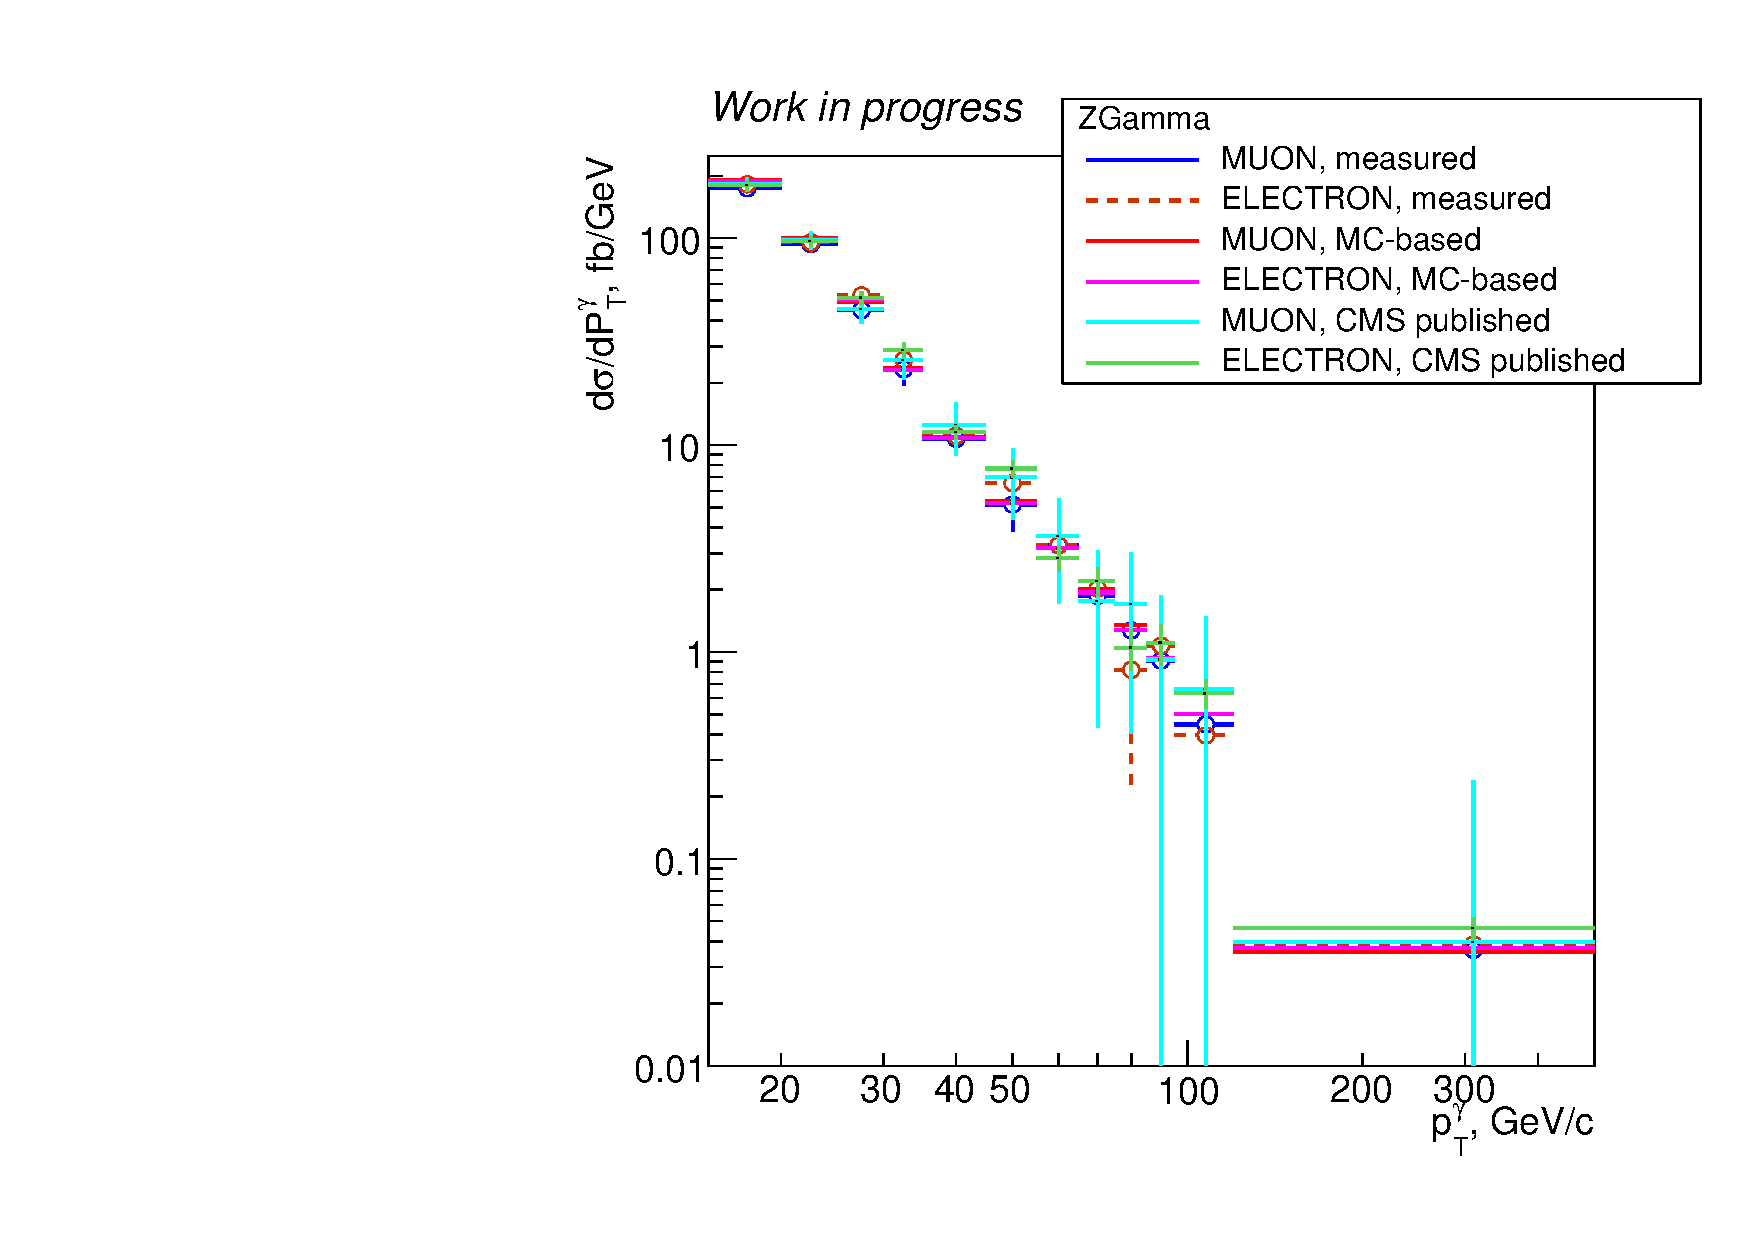
\includegraphics[width=0.48\textwidth]{../figs/figs_v11/ChannelsMERGED_ZGamma/CrossSection/compareCSZGamma.pdf}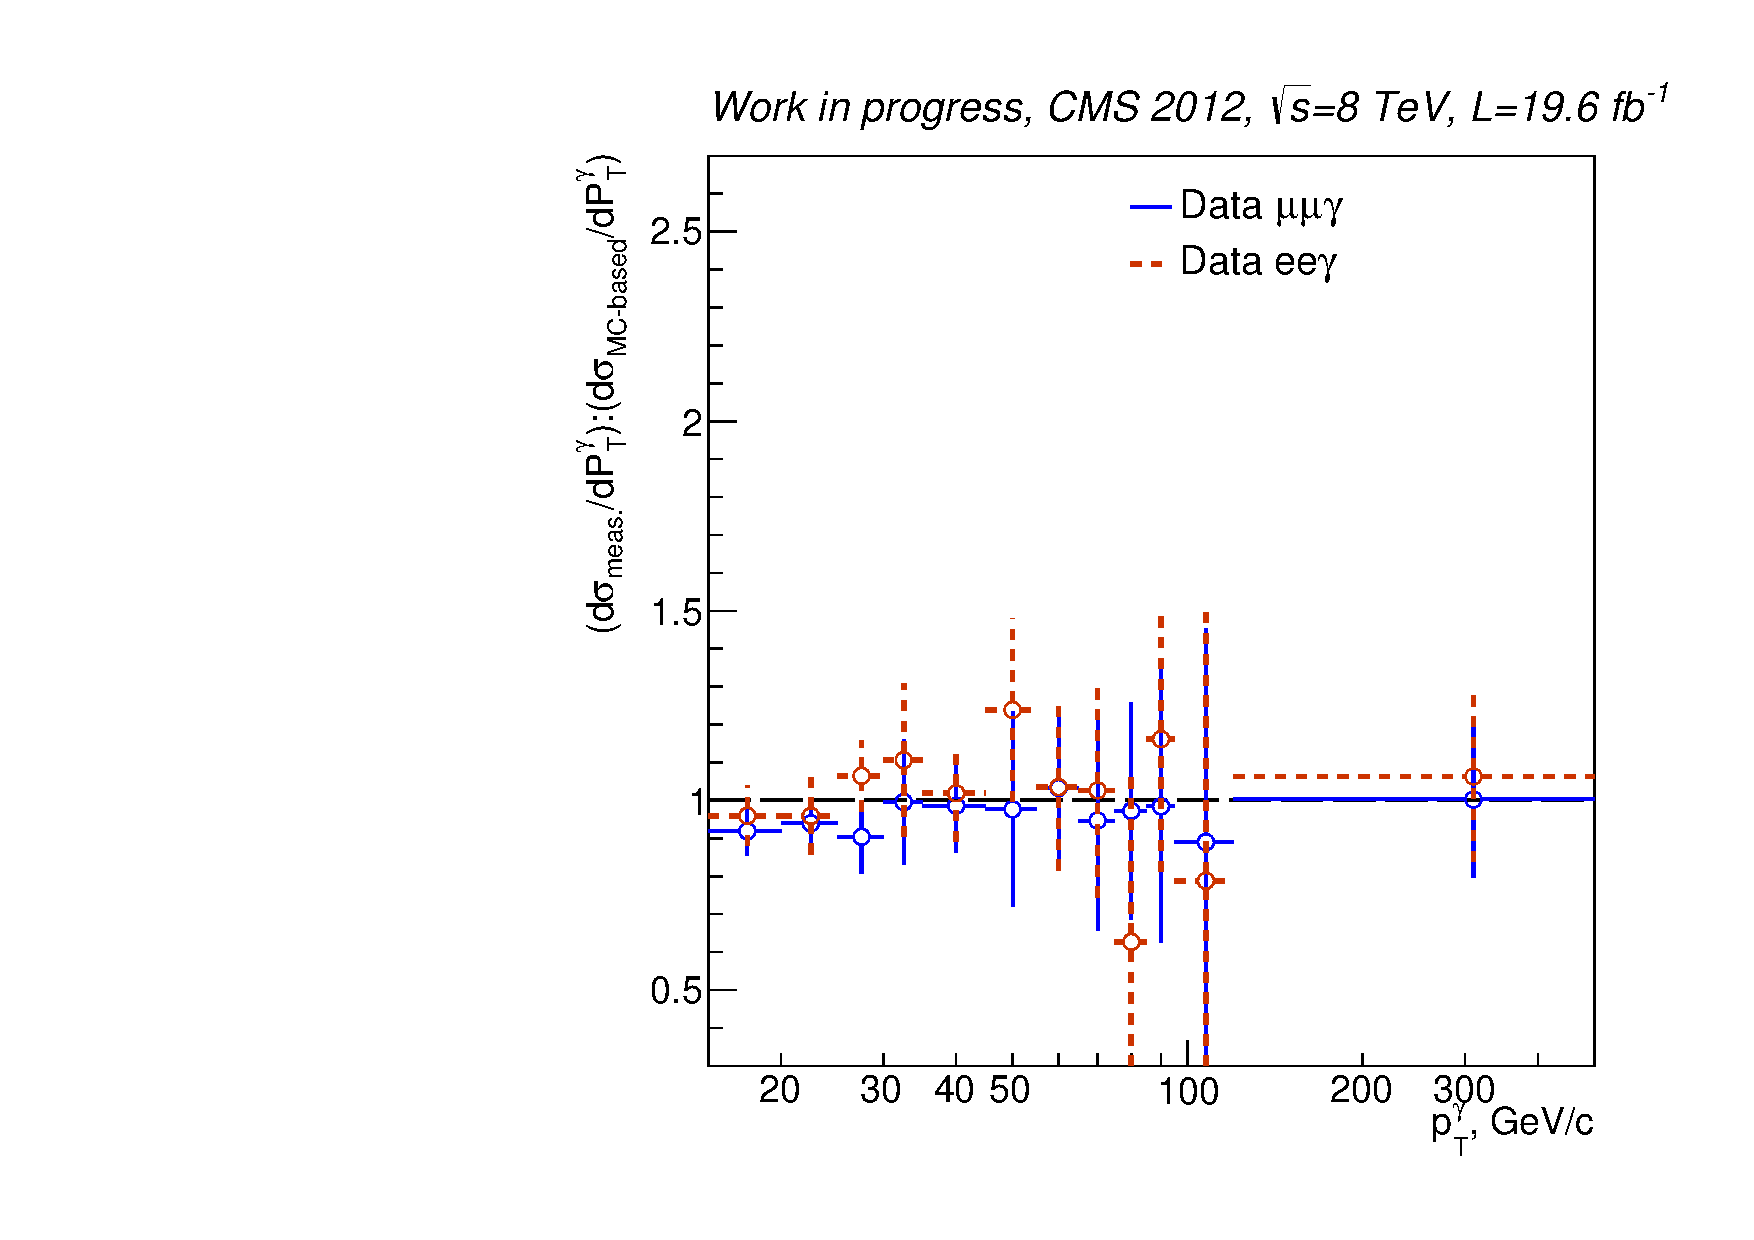
\includegraphics[width=0.48\textwidth]{../figs/figs_v11/ChannelsMERGED_ZGamma/CrossSection/compareCSratioTheoryZGamma.pdf}
   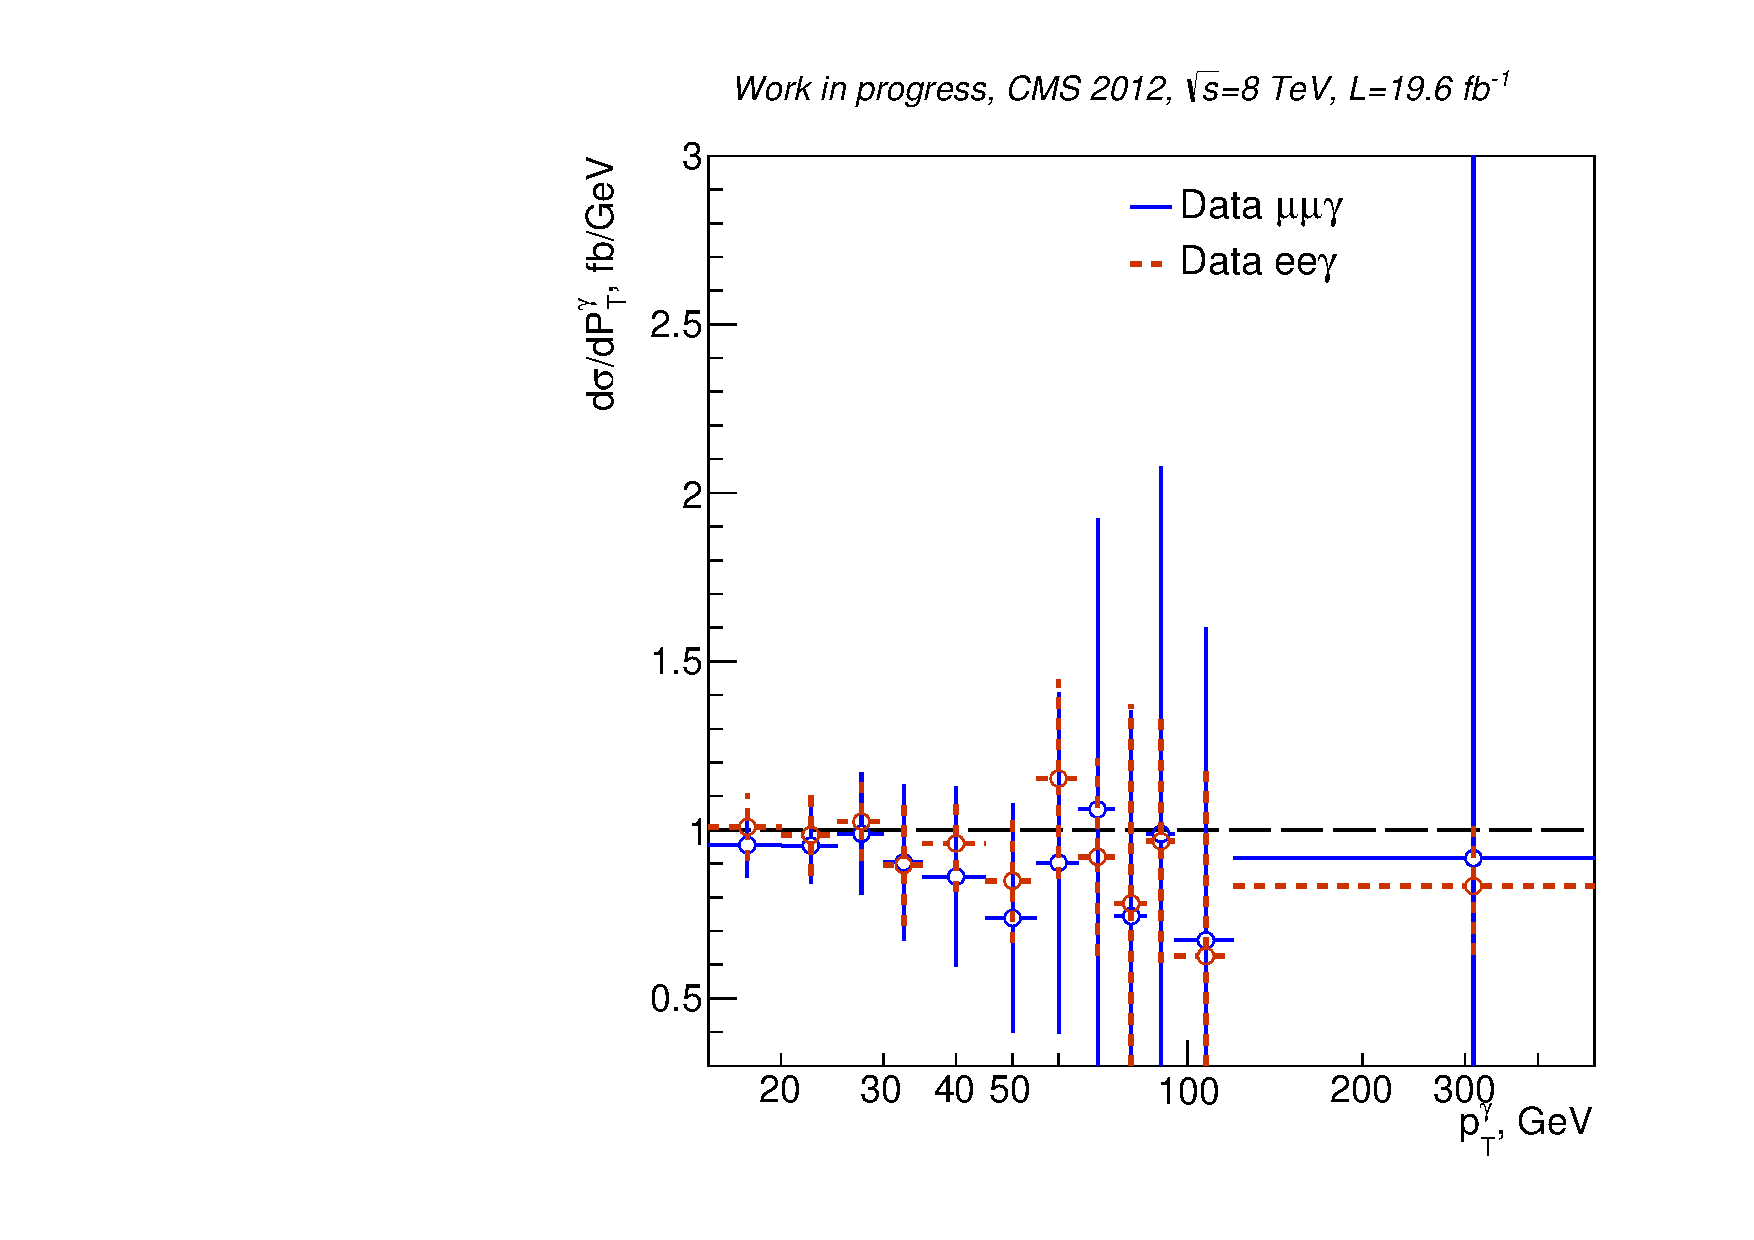
\includegraphics[width=0.48\textwidth]{../figs/figs_v11/ChannelsMERGED_ZGamma/CrossSection/compareCSratioOttoZGamma.pdf}
     
  \caption{Top left: the $Z\gamma$ differential cross section; top right: the ratio of measured over the NLO theory $Z\gamma$ differntial cross section; bottom: the ratio of the measured over the CMS published $Z\gamma$ differential cross section. }
  \label{fig:CS_Zg}
 \end{center}
\end{figure}

  \begin{table}[h]
  \scriptsize
  \begin{center}
  \caption{Cross section and errors}
  \begin{tabular}{|c|c|c|c|}
                     & \multicolumn{3}{|c|}{$d\sigma/dP_{T}^{\gamma}$, fb/GeV} \\ 
     $P_T^{\gamma}$, & NLO theory                          &  \multicolumn{2}{|c|}{measured}      \\
    GeV              &  $Z\gamma\rightarrow ll\gamma$ & $Z\gamma\rightarrow \mu\mu\gamma$  & $Z\gamma\rightarrow ee\gamma$    \\ \hline
    total & 2073 & 1938 $\pm$ 20 $\pm$ 78 & 2058 $\pm$ 27 $\pm$ 93\\ \hline
%    10-15 & 359 & 326 $\pm$ 7 $\pm$ 33  & 339 $\pm$ 9 $\pm$ 26\\ \hline
    15-20 & 190 & 174 $\pm$ 3 $\pm$ 12 & 182 $\pm$ 5 $\pm$ 14\\ \hline
    20-25 & 100 & 94 $\pm$ 2 $\pm$ 5 & 96 $\pm$ 3 $\pm$ 10\\ \hline
    25-30 & 50 & 45 $\pm$ 1 $\pm$ 5 & 53 $\pm$ 2 $\pm$ 4\\ \hline
    30-35 & 23 & 23 $\pm$ 1 $\pm$ 4 & 26 $\pm$ 1 $\pm$ 5\\ \hline
    35-45 & 11 & 11 $\pm$ 0 $\pm$ 1 & 11 $\pm$ 1 $\pm$ 1\\ \hline
    45-55 & 5.3 & 5.2 $\pm$ 0.4 $\pm$ 1.3 & 6.5 $\pm$ 0.5 $\pm$ 1.2\\ \hline
    55-65 & 3.2 & 3.3 $\pm$ 0.2 $\pm$ 0.6 & 3.3 $\pm$ 0.3 $\pm$ 0.6\\ \hline
    65-75 & 2.0 & 1.9 $\pm$ 0.2 $\pm$ 0.5 & 2.0 $\pm$ 0.3 $\pm$ 0.5\\ \hline
    75-85 & 1.3 & 1.3 $\pm$ 0.2 $\pm$ 0.3  & 0.82 $\pm$ 0.21 $\pm$ 0.55\\ \hline
    85-95 & 0.92 & 0.91 $\pm$ 0.15 $\pm$ 0.30 & 1.1 $\pm$ 0.2 $\pm$ 0.3 \\ \hline
    95-120 & 0.50 & 0.45 $\pm$ 0.09 $\pm$ 0.27 & 0.40 $\pm$ 0.11 $\pm$ 0.34\\ \hline
    120-500 & 0.036 & 0.036 $\pm$ 0.003 $\pm$ 0.007 & 0.039 $\pm$ 0.004 $\pm$ 0.007 \\ \hline
  \end{tabular}
  \label{tab:cs_mc_vs_meas_ZGamma}
  \end{center}
\end{table}
